%%%%%%%%%%%%%%%%%%%%%%%%%%%%%%%%%%%%%%%%%
% eBook
% LaTeX Template
% Version 1.0 (29/12/14)
%
% This template has been downloaded from:
% http://www.LaTeXTemplates.com
%
% Original author:
% Luis Cobo (luiscobogutierrez@gmail.com) with extensive modifications by:
% Vel (vel@latextemplates.com)
%
% License:
% CC BY-NC-SA 3.0 (http://creativecommons.org/licenses/by-nc-sa/3.0/)
%
%%%%%%%%%%%%%%%%%%%%%%%%%%%%%%%%%%%%%%%%%

%----------------------------------------------------------------------------------------
%	DOCUMENT CONFIGURATIONS AND INFORMATION
%----------------------------------------------------------------------------------------

\documentclass[oneside,11pt]{memoir} % Font size

%%%%%%%%%%%%%%%%%%%%%%%%%%%%%%%%%%%%%%%%%
% eBook
% Structural Definitions File
% Version 1.0 (29/12/14)
%
% Created by:
% Vel (vel@latextemplates.com)
%
% This file has been downloaded from:
% http://www.LaTeXTemplates.com
%
% License:
% CC BY-NC-SA 3.0 (http://creativecommons.org/licenses/by-nc-sa/3.0/)
%
%%%%%%%%%%%%%%%%%%%%%%%%%%%%%%%%%%%%%%%%%

%----------------------------------------------------------------------------------------
%	REQUIRED PACKAGES
%----------------------------------------------------------------------------------------

\usepackage[utf8]{inputenc} % Required for inputting international characters
\usepackage[T1]{fontenc} % Output font encoding for international characters

\usepackage[osf]{libertine} % Use the Libertine font
\usepackage{microtype} % Improves character and word spacing

\usepackage{tikz} % Required for drawing custom shapes
\definecolor[named]{color01}{rgb}{.2,.4,.6} % Color used in the title page
\usepackage{wallpaper} % Required for setting background images (title page)

\usepackage[unicode=true,bookmarks=true,bookmarksnumbered=false,bookmarksopen=false,breaklinks=false,pdfborder={0 0 1},backref=section,colorlinks=false, hidelinks = True]{hyperref} % PDF meta-information specification

\usepackage{enumitem}
\usepackage{xparse}
\usepackage{epigraph} % for quote
\usepackage{amsmath}
\usepackage{subcaption}
\usepackage{csvsimple}
\setcounter{tocdepth}{2}
\setcounter{secnumdepth}{2}

%----------------------------------------------------------------------------------------
%	Python code format
%----------------------------------------------------------------------------------------
\usepackage[T1]{fontenc}
\usepackage{fourier}

\usepackage[scaled=0.8]{beramono}
\usepackage{listings}
\usepackage{color}
\definecolor{deepblue}{rgb}{0,0,0.5}
\definecolor{deepred}{rgb}{0.6,0,0}
\definecolor{deepgreen}{rgb}{0,0.5,0}

\lstset{
  language=Python,
  showstringspaces=false,
  formfeed=\newpage,
  tabsize=4,
  commentstyle=\color{deepgreen}\itshape,
  basicstyle=\ttfamily\footnotesize\color{deepblue},
  stringstyle=\color{deepred},
  keywordstyle=\color{deepblue},
  morekeywords={models, lambda, forms},
}
\newcommand{\code}[2]{%
  \hrulefill
  \subsection*{#1}%
  \lstinputlisting{#2}%
  \vspace{2em}%
}
%----------------------------------------------------------------------------------------


%----------------------------------------------------------------------------------------
%	exam paper format
%----------------------------------------------------------------------------------------
%Idea from https://tex.stackexchange.com/a/236668/1952
\DeclareDocumentCommand\question{o}{%
    \item\IfNoValueTF{#1}{}{(#1 points)}}

\newenvironment{questions}[1][]{\enumerate[,#1]}{\endenumerate}

\newlist{oneparchoices}{enumerate*}{1}
\setlist[oneparchoices,1]{label=\Alph*., itemjoin={{\quad}}}

\newcommand{\choice}{\item}
%----------------------------------------------------------------------------------------
%	PAPER, MARGIN AND HEADER/FOOTER SIZES
%----------------------------------------------------------------------------------------

\setstocksize{20.3cm}{25.4cm} % Paper size
\settrimmedsize{\stockheight}{\stockwidth}{*} % No trims
\setlrmarginsandblock{3cm}{3cm}{*} % Left/right margins
\setulmarginsandblock{4.5cm}{4.5cm}{*} % Top/bottom margins
\setheadfoot{14pt}{12pt} % Header/footer height
\setheaderspaces{*}{8pt}{*} % Extra header space

%----------------------------------------------------------------------------------------
%	FOOTNOTE CUSTOMIZATION
%----------------------------------------------------------------------------------------

\renewcommand{\foottextfont}{\itshape\footnotesize} % Font settings for footnotes
\setlength{\footmarkwidth}{-.1em} % Space between the footnote number and the text
\setlength{\footmarksep}{.1em} % Space between multiple footnotes on the same page
\renewcommand*{\footnoterule}{} % Remove the rule above the first footnote
\setlength{\skip\footins}{1\onelineskip} % Space between the body text and the footnote

%----------------------------------------------------------------------------------------
%	HEADER AND FOOTER FORMATS
%----------------------------------------------------------------------------------------

\makepagestyle{mio} % Define a new custom page style
\setlength{\headwidth}{\textwidth} % Header the same width as the text
\makeheadrule{mio}{\textwidth}{0.1mm} % Header rule height
\makeoddhead{mio}{\scriptsize{\theauthor\hskip.2cm\vrule\hskip.2cm\itshape{\thetitle}}}{}{} % Header specification
\makeoddfoot{mio}{}{\scriptsize {\thepage \quad \vrule \quad \thelastpage}}{} % Footer specification
\makeoddfoot{plain}{}{\footnotesize {\thepage \quad \vrule \quad \thelastpage}}{} % Pages of chapters
\pagestyle{mio} % Set the page style to the custom style defined above

%----------------------------------------------------------------------------------------
%	PART FORMAT
%----------------------------------------------------------------------------------------

\renewcommand{\partnamefont}{\centering\sffamily\itshape\Huge} % Part name font specification
\renewcommand{\partnumfont}{\sffamily\Huge} % Part number font specification
\renewcommand{\parttitlefont}{\centering\sffamily\scshape} % Part title font specification
\renewcommand{\beforepartskip}{\null\vskip.618\textheight} % Whitespace above the part heading

%----------------------------------------------------------------------------------------
%	CHAPTER FORMAT
%----------------------------------------------------------------------------------------

\makechapterstyle{Tufte}{ % Define a new chapter style
\renewcommand{\chapterheadstart}{\null \vskip3.5\onelineskip} % Whitespace before the chapter starts
\renewcommand{\printchaptername}{\large\itshape\chaptername} % "Chapter" text font specification
\renewcommand{\printchapternum}{\LARGE\thechapter \\} % Chapter number font specification
\renewcommand{\afterchapternum}{} % Space between the chapter number and text
\renewcommand{\printchaptertitle}[1]{ % Chapter title font specification
\raggedright
\itshape\Huge{##1}}
\renewcommand{\afterchaptertitle}{
\vskip3.5\onelineskip
}}
\chapterstyle{Tufte} % Set the chapter style to the custom style defined above

%----------------------------------------------------------------------------------------
%	SECTION FORMAT
%----------------------------------------------------------------------------------------

\setsecheadstyle{\sethangfrom{\noindent ##1}\raggedright\sffamily\itshape\Large} % Section title font specification
\setbeforesecskip{-.6\onelineskip} % Whitespace before the section
\setaftersecskip{.3\onelineskip} % Whitespace after the section

%----------------------------------------------------------------------------------------
%	SUBSECTION FORMAT
%----------------------------------------------------------------------------------------

\setsubsecheadstyle{\sethangfrom{\noindent  ##1}\raggedright\sffamily\large\itshape} % Subsection title font specification
\setbeforesubsecskip{-.5\onelineskip} % Whitespace before the subsection
\setaftersubsecskip{.2\onelineskip} % Whitespace after the subsection

%----------------------------------------------------------------------------------------
%	SUBSUBSECTION FORMAT
%----------------------------------------------------------------------------------------

\setsubsubsecheadstyle{\sethangfrom{\noindent ##1}\raggedright\sffamily\itshape} % Subsubsection title font specification
\setbeforesubsubsecskip{-.5\onelineskip} % Whitespace before the subsubsection
\setaftersubsubsecskip{.1\onelineskip} % Whitespace after the subsubsection

%----------------------------------------------------------------------------------------
%	CAPTION FORMAT
%----------------------------------------------------------------------------------------

\captiontitlefont{\itshape\footnotesize} % Caption font specification
\captionnamefont{\footnotesize} % "Caption" text font specification

%----------------------------------------------------------------------------------------
%	QUOTATION ENVIRONMENT FORMAT
%----------------------------------------------------------------------------------------

\renewenvironment{quotation}
{\par\leftskip=1em\vskip.5\onelineskip\em}
{\par\vskip.5\onelineskip}

%----------------------------------------------------------------------------------------
%	QUOTE ENVIRONMENT FORMAT
%----------------------------------------------------------------------------------------

\renewenvironment{quote}
{\list{}{\em\leftmargin=1em}\item[]}{\endlist\relax}

%----------------------------------------------------------------------------------------
%	MISCELLANEOUS DOCUMENT SPECIFICATIONS
%----------------------------------------------------------------------------------------

\setlength{\parindent}{1em} % Paragraph indentation

\midsloppy % Fewer overfull lines - used in the memoir class and allows a setting somewhere between \fussy and \sloppy

\checkandfixthelayout % Tell memoir to implement the above  % Include the file that specifies the document structure and layout

\title{Introduction to Deep Learning} % Book title
\author{Dr Myo Thida} % Author
\newcommand{\edition}{} % Book edition

%----------------------------------------------------------------------------------------

\begin{document}

%----------------------------------------------------------------------------------------
%	TITLE PAGE
%----------------------------------------------------------------------------------------

\thispagestyle{empty} % Suppress page numbering
\ThisCenterWallPaper{1.5}{imgs/DL_cover2.png}

\newpage % Make sure the following content is on a new page
\begin{tikzpicture}[remember picture,overlay]
\end{tikzpicture}

\newpage
\vspace*{5cm}
% Sets a PDF bookmark for the dedication
\pdfbookmark{Dedication}{dedication}
\thispagestyle{empty}
\begin{center}
   \emph{This book is dedicated to my students over the years and to the brave youths of Myanmar, who have infused me with unwavering courage and energy, inspiring me to persevere.}
\end{center}

\newpage

\vspace*{\fill}
\small
Copyright \textcopyright\ 2024 by VigorZwe Co. Ltd. All rights reserved.
No part of this book may be reproduced or reprinted without permission in writing from the publisher or the author.
\newpage

%----------------------------------------------------------------------------------------
%	TABLE OF CONTENTS
%----------------------------------------------------------------------------------------

\tableofcontents % Prints the table of contents

%----------------------------------------------------------------------------------------
%	PREFACE
%----------------------------------------------------------------------------------------

\chapter*{Preface}

%The terms 'AI,' 'deep learning,' and 'machine learning' are not unfamiliar to me, as I am trained as a computer vision and machine learning scientist. My PhD research, which focused on analyzing the contextual information of videos using traditional machine learning techniques, remains relevant, with many readers still citing it as foundational work. However, I took a career hiatus of approximately six years to contribute to the national development of Myanmar. Upon returning to the technological landscape in 2019, I experienced stress and anxiety, fearing I had fallen behind.
%
%Determined to catch up, I quickly familiarized myself with new terminologies and found learning to be more manageable, perhaps due to my increased maturity and experience collaborating with industry professionals. This newfound clarity enabled me to communicate complex concepts more effectively, as evidenced by the success of my previous work, 'Introduction to Supervised Machine Learning (2023),' which sold over 100 copies within a year. Moreover, receiving positive feedback from readers about the accessibility and clarity of my explanations motivated me to embark on writing this teaching book: 'Introduction to Deep Learning.'

My interest in AI began in 2003 when I completed a literature review on face recognition methods as my first undergraduate research project. This project sparked my passion for computer vision and machine learning, leading me to pursue both a Master's and a PhD in the field. Throughout my academic journey, I published research in journals and authored a book titled 'Contextual Analysis of Videos,' all written in English.

Over time, I became aware of the challenges faced by many Myanmar students, who had limited access to quality books due to language barriers and found most available resources too advanced. This realization inspired me to write technology books in Burmese using my own teaching style. My first book, 'Introduction to MATLAB: Learning by Doing,' was published in 2008. The second book, 'Introduction to Supervised Machine Learning,' written in both English and Burmese, was published in 2023. Encouraged by positive feedback on the accessibility and clarity of my explanations, I embarked on writing this teaching book: 'Introduction to Deep Learning.'

This book emerged from one of the most challenging periods of my life, during which the tumultuous situation in Myanmar weighed heavily on my mind, particularly witnessing the struggles of many young people. The purpose of this book is not only to make deep learning accessible to students with limited resources but also to contribute to the support of youths in need. 

This book is structured into four parts to facilitate a comprehensive understanding of deep learning concepts and methodologies. The first chapter serves as a foundational introduction to deep machine learning algorithms. It covers the historical evolution of deep learning, essential mathematical concepts, and prerequisites necessary to comprehend the subsequent chapters.  It also introduces Python libraries commonly used for deep learning, such as TensorFlow and Keras.

Chapter two delves into the architecture and functioning of shallow neural networks. It covers topics such as activation functions, forward and backward propagation, and model optimization techniques. Practical projects demonstrating the application of shallow NNs in regression, binary classification, and multi-class classification tasks are included.  Chapter three explores advanced deep learning architectures, including convolutional neural networks (CNNs), recurrent neural networks (RNNs), and their variants. It discusses the principles behind these architectures and their applications in computer vision, natural language processing, and time-series data analysis.

Chapter four delves into specialized topics and emerging trends in deep learning. It covers areas such as transfer learning, attention mechanisms, AutoML, neural architecture search (NAS), and ethical considerations in deep learning. Through case studies and discussions, this chapter provides insights into advanced methodologies and ethical considerations shaping the future of deep learning.

I believe that hands-on learning is crucial for understanding, and thus, the explanations in the book are accompanied by detailed 'Python code' snippets throughout the text. Readers can follow the instructions and run the code on their own computer or an online platform such as Google Colab.

As you delve into the chapters that follow, I encourage you to approach this journey with an open mind and a spirit of exploration. Whether you are a seasoned expert in the field or a curious novice, there is something to be gained from the insights contained within these pages.

The website: \href{www.drmyothida.org/courses}{www.drmyothida.org/courses/machinelearning}. The complete code for all the projects in this book is also available on the public \href{https://github.com/myothida/Intro-To-Supervised-Machine-Learning.git}{\textbf{GitHub Repo}}.

\chapter*{စာညွှန်း}

စာရေးသူမှာ စင်ကာပူနိုင်ငံ နန်ယန်း တက္ကသိုလ်တွင် အင်ဂျင်နီယာ ဘွဲ့ကြိုသင်တန်းအား ၂၀၀၁ မှ ၂၀၀၅ ခုနှစ်ထိ တတ်ရောက်ခဲ့ပါသည်။ ထိုဘွဲ့ကြိုသင်တန်းကာလအတွင်း ပြုလုပ်ခဲ့သည့် "Literature Review on Face Recognition Methods" ဟုခေါ်ဆိုသည့် စာတမ်းငယ် မှာ စာရေးသူ၏ ပထမဦးဆုံး မှတ်ဥာဏ်အတု Artificial Intelligence (AI) နှင့် ပတ်သတ်သည့် သုတေသန လုပ်ငန်းစဥ် တစ်ခု ဖြစ်ခဲ့ပါသည်။ ထိုသုတေသနမှ အစပြု၍ computer vision နှင့် machine learning ကို ပိုမို စိတ်၀င်စားလာကာ Computer Vision ဘာသာရပ်ကို အထူးပြု၍ မာစတာနှင့် ဒေါက်တာ ဘွဲ့များကို ဆက်လက် ရယူခဲ့ပါသည်။ သုတေသန စာတမ်းငယ်များစွာနှင့် Contextual Analysis of Videos နည်းပညာစာအုပ်ကို အင်္ဂလိပ်ဘာသာဖြင့်  ရေးသား ထုတ်၀ေခဲ့သည်။

၂၀၁၃ ခုနှစ် နှောင်းပိုင်းတွင် မြန်မာနိုင်ငံသို့ ပြန်ရောက်ပြီးနောက် မြန်မာလူငယ်များကို   computer vision နှင့် machine learning ဆိုင်ရာ ဘာသာရပ်များကို သင်ကြားဖြစ်ရင်းမှ အင်္ဂလိပ်ဘာသာစကားဖြင့် ထုတ်၀ေသည့် စာအုပ်များကို မြန်မာ လူငယ်များ (အထူးသဖြင့် အင်္ဂလိပ်စာ ဘာသာစကား အားနည်းသော လူငယ်များ ) အတွက် ဖတ်ရှု့လေ့လာရန် ခက်ခဲလျက်ရှိသည်ကို သိရှိလာရသည်။ သို့ဖြစ်ရာ ရိုးရှင်းသည့် စကားလုံးများကို အသုံးပြု၍ မြန်မာသာသာဖြင့် နည်းပညာစာအုပ်များကို သင်ကြားရေးတွင် အသုံးပြုရန် စတင် ရေးသားခဲ့ပါသည်။ ထို့နောက် ၂၀၁၈ ခုနှစ်တွင် Introduction to MATLAB: Learning by Doing စာအုပ်ကို လည်းကောင်း၊ ၂၀၂၃ ခုနှစ်တွင်  Introduction to Supervised Machine Learning စာအုပ်ကို လည်းကောင်း ရေးသားထုတ်၀ေခဲ့သည်။ 

ယခု ရေးသားထုတ်၀ေမည့် Introduction to Deep Learning နှင့်  ၂၀၂၃ ခုနှစ်တွင် ထုတ်၀ေခဲ့သည့် Introduction to Supervised Machine Learning - စာအုပ် ၂ အုပ်လုံးမှာ ကျွန်မ ဘ၀၏ စိတ်သောက အများဆုံး အချိန်တွင် ရေးသားခဲ့သည့် စာအုပ်များဖြစ်သည်ဟု ဆိုနိုင်ပါသည်။ လက်ရှိ မြန်မာနိုင်ငံ၏ အခြေအနေများမှာ ပညာရေးဖြင့် တိုင်းပြည်ကို တိုးတက်စေချင်သူ ကျွန်မအတွက် စိတ်ဖိစီးမှု များစွာ ဖြစ်စေပါသည်။ သို့သော် ခက်ခဲနေသည့် အခြေအနေများ အကြားတွင်ပင် မလျှော့သော ဇွဲ၊ လုံ့လဖြင့် ကြိုးစားနေကြသည့် မြန်မာ လူငယ်များမှ ပေးသောခွန်အားဖြင့် ဤနည်းပညာစာအုပ်များကို ရေးသားခဲ့ပါသည်။  ယခု စာအုပ်သည် အခြားနိုင်ငံသားများနည်းတူ မြန်မာ လူငယ်များလည်း နည်းပညာကို အမီလိုက်နိုင်စေရန် ရည်ရွယ်ရေးသားခြင်း ဖြစ်သည်။ နှလုံးသားနှင့် ဦးဏှောက် စည်းချက်ညီစွာဖြင့် ကြိုးစားနေကြသော မြန်မာ လူငယ်၊ လူရွယ် (ဆယ်လ်မွန်ငါး) များအတွက် အလွယ်တကူ ဖတ်ရှု့နိုင်သည့် နည်းပညာ စာအုပ်တစ်အုပ်အဖြစ် ပညာဖြန့်၀ေနိုင်ရန် ရည်ရွယ်ပါသည်။ 

ယခု စာအုပ်တွင် အပိုင်း ၄ ပိုင်းပါ၀င်ပြီး ပထမ အပိုင်းမှာ Deep Learning ကို မိတ်ဆက်ခြင်း ဖြစ်ပါသည်။ သို့သော် Machine Learning / AI စသည့် အခြေခံ သဘောတရားများကို ပြန်လည်ရှင်းပြခြင်းထက်  Deep Learning ၏ သဘောတရားများကို တိုက်ရိုက်မိတ်ဆက်သွားမည် ဖြစ်ရာ AI / Machine Learning စသည့် နည်းပညာ စကားလုံးများနှင့် ၀ေးကွာနေသူများအဖို့  ဤစာအုပ်ကိုမဖတ်မီ  Introduction to Supervised Machine Learning ကို ဖတ်ရှု့ရန် တိုက်တွန်းပါသည်။ Deep Learning ကို လေ့လာရာတွင် အရေးကြီးသည့် အချို့ သင်္ချာ ခေါင်းစဥ်များနှင့် ယခု စာအုပ်တွင် အသုံးပြုသွားမည့်  Python Library များကိုလည်း ပထမ အပိုင်းတွင် မိတ်ဆက်ထားပါသည်။ 

ဒုတိယအခန်းတွင်  Deep Learning ၏ မူလ အခြေခံဖြစ်သည့် Shallow Neural Network ကို ရှင်းပြသွားမည်ဖြစ်ပြီး လက်တွေ့ လေ့ကျင့်ခန်းများကို လည်း Python Code များနှင့်အတူ ဆွေးနွေးပေးသွားမည် ဖြစ်သည်။ ထို့နောက် တတိယ အခန်းတွင်မူ ပိုမို အဆင်မြင့်သည့် Deep Learning Architecture အမျိုးမျိုးကို ရှင်းလင်းသွားပြီး Convolutional Neural Networks (CNNs)၊ Recurrent Neural Networks (RNNs) များကို အသုံးပြု၍ Image များ  Text များကို အမျိုးအစား ခွဲခြားပုံများကို ဆွေးနွေးသွားပါမည်။ နောက်ဆုံးအပိုင်းတွင်မူ Deep Learning ၏ နောက်ဆုံး ပြောင်းလဲလျက်ရှိသည့် ခေါင်းစဥ်များနှင့် ဆက်လက်လေ့လာရမည်များကို ဆွေးနွေးသွားပါမည်။ 

ယခု စာအုပ်ကို အင်္ဂလိပ် - မြန်မာ ၂ ဘာသာဖြင့် ရေးသားထားပြီး စာမျက်နှာအလိုက် တွဲ၍ ဖတ်ရှု့သွားနိုင်မည် ဖြစ်သည်။ တိုက်ရိုက် ဘာသာပြန်ဆိုထားခြင်း မဟုတ်ဘဲ စာသားပြေပြစ်စေရန် အဓိက ရေးသားထားသည် ဖြစ်ရာ ဘာသာစကား တစ်ခုထဲကို အသုံးပြု ဖတ်ရှု့သူများ အနေဖြင့် အကျိုးရှိနိုင်သကဲ့သို့ ဘာသာစကား ၂ ခုလုံးကို တွဲ၍ ဖတ်ရှု့ပါကလည်း ပို၍ အကျိုးများနိုင်ပါသည်။ 

နည်းပညာစာအုပ်များကို ဖတ်ရှု့ရာတွင် အမှန်တကယ် နားလည်လိုသည်ဆိုပါက လက်တွေ့ လေ့ကျင့်ခန်းများနှင့် တွဲ၍ ဖတ်ရှု့ရန် လိုအပ်ပါသည်။ ဤစာအုပ်တွင် ပါရှိသည့် Python ဖြင့်ရေးသားထားသည့် လေ့ကျင့်ခန်းများကို အောက်ပါ \href{https://github.com/myothida/Intro-To-Supervised-Machine-Learning.git}{\textbf{GitHub}} လင့်တွင် ၀င်ရောက်၍ download ရယူပြီးလေ့ကျင့်စေလိုပါသည်။ 

%----------------------------------------------------------------------------------------
%	CHAPTER ONE
%----------------------------------------------------------------------------------------

%----------------------------------------------------------------------------------------
%	CHAPTER ONE
%----------------------------------------------------------------------------------------

\chapter{Introduction to Deep Learning}
Deep learning is rooted in the concept of artificial neural networks (ANNs), which are computing systems inspired by the biological neural networks of the human brain. The basic idea dates back to the 1940s and 1950s when researchers began exploring the mathematical models of neurons. Yann LeCun's work in the 1980s, particularly his development of convolutional neural networks (CNNs)  \cite{lecun1989}, played a crucial role in advancing neural network research. However, despite these advancements, neural network research faced challenges, including limited computational power and insufficient data, leading to a period of stagnation during the 1970s and 1980s.

The breakthroughs that led to the modern era of deep learning began around the mid-2000s. The term ``deep learning" gained widespread recognition around 2012 when deep neural networks, particularly convolutional neural networks (CNNs)  \cite{krizhevsky2012ImageNet}, achieved ground-breaking performance in computer vision tasks, such as image classification, through competitions like the ImageNet Large Scale Visual Recognition Challenge (ILSVRC) \cite{web:ILSVRC}.

\section{Mathematics for Deep Learning}
It is crucial to have mathematical fundamentals to fully comprehend deep learning concepts. This section offers an overview of essential mathematical topics necessary for delving into deep learning algorithms. To fully grasp the content of this book on deep learning, it is essential for students to have a basic understanding of the following mathematical topics:

\begin{itemize}
  \item \textbf{Linear Algebra}: Linear algebra forms the foundation of many deep learning techniques. Concepts such as vectors, matrices, matrix operations (addition, multiplication), matrix factorization (e.g., Singular Value Decomposition), and eigenvalues/eigenvectors are important.
  \item \textbf{Calculus}: Calculus plays a vital role in understanding optimization algorithms used in training deep learning models. Concepts like derivatives, gradients, chain rule, optimization techniques (e.g., gradient descent, stochastic gradient descent), and convex optimization are essential.
  \item \textbf{Probability and Statistics}: Probability theory is important for understanding the uncertainty associated with data and predictions in deep learning models. Concepts like probability distributions (e.g., Gaussian distribution), expected value, variance, covariance, conditional probability, Bayes' theorem, and statistical inference are crucial.
  \item \textbf{Graph Theory}: Graph theory is relevant for understanding neural network architectures and operations. Concepts like directed and undirected graphs, nodes, edges, adjacency matrices, and graph algorithms (e.g., breadth-first search, depth-first search) are important for understanding the structure and behavior of neural networks.
\end{itemize}

\section{Artificial Neural Networks}

\subsection{Feedforward Neural Networks}
These are the simplest form of neural networks, consisting of an input layer, one or more hidden layers, and an output layer. Each neuron in one layer is connected to every neuron in the next layer, with no feedback connections.

\section{Different Deep Learning Algorithms}

Deep learning algorithms typically involve neural networks with multiple layers (hence the term "deep"), allowing them to automatically discover intricate patterns and representations from raw data. This section introduces some common types of deep learning algorithms:

\subsection{Convolutional Neural Network}
The example of "teaching a child to speak their first word" illustrates a supervised machine learning problem. This type of machine learning requires a pre-existing data-set with known information and desired outcomes. The machine learning model must learn from this dataset in order to predict the desired outcome.

Supervised machine learning is widely used in today's technologies across various fields such as bio-security, weather forecasting, text prediction, and spam detection, etc. These methods use pre-existing data that includes both input features and the desired output (or target variable) to understand the underlying relationship. The model learns from the data, and the resulting parameters can be used to predict outcomes for new data.

An example of supervised learning is a biometric authentication system that uses facial recognition or fingerprints for logging into computers or mobile phones. The system is trained to recognize an individual's unique bio-data through registration. Once registered, the system compares presented bio-data to the registered information, and grants ("accept") or denies access ("reject") accordingly. Another example is a weather forecasting system that provides numerical data as output.

Depending on the type of output, supervised learning methods can be divided into two categories: \textbf{classification}, which assigns a class label to new data (such as "accept" or "reject") and \textbf{regression}, which predicts a numerical value (such as weather data).

\subsection{Recurrent Neural Network}
Unsupervised machine learning refers to the process of analyzing data without a pre-existing labeled dataset. In this case, the machine learning method extracts information from the data on its own.

For example, imagine you are an active user of a social media page and your team has been uploading photos regularly for over a decade. One day, you decide to download all the photos and sort them based on similar activities. Manually checking and labeling each photo would be time-consuming as there are more than 100,000 photos. Unsupervised machine learning can be used to analyze and group the photos into different clusters based on similarity measures. Photos in the same group will be more alike than those in different groups.

To sum up, unsupervised machine learning methods focus on analyzing and grouping a large dataset into different clusters, based on user-defined rules of association. Another common use of unsupervised machine learning is anomaly detection, where the data is divided into normal (majority) and abnormal (outlier) groups.

\subsection{Long Short-Term Memory (LSTM)}

Reinforcement learning is a field of machine learning, in which an agent learns to perform tasks by trial-and-error, while receiving feedback in form of reward signals. Referring to the example of learning our first word, we start saying "mama" after learning from our parents, but sometimes we make mistakes and our parents help correct us by giving rewards for saying the right word or scolding us when we are wrong.

Similarly, reinforcement learning methods learn by interacting with their environment and receiving positive or negative feedback. Reinforcement learning is often used in training robots for navigation.

\subsection{Generative Adversarial Network}

\newpage
\section{Introduction to Python Environment}

While there are many programming languages to choose from, the ones widely used in deep learning include Python, R, C, and Java. Proficiency in programming languages is a fundamental skill in the journey of understanding deep learning. In this course, we will use Python \cite{web:python} to develop deep learning algorithms. Python is an open-source programming language, it is easy to learn and there are a plenty of libraries and frameworks specifically designed for machine learning and deep learning. There are several Integrated Development Environments (IDEs) to write Python code and Jupyter Notebook \cite{web:juypter} is one of the most popular choices among deep learning practitioners and professors. Additionally, Google Colab \cite{web:googlecolab} is a free cloud service offered by Google, which allows you to run Jupyter Notebooks online without installing it on your computer and access the computing resources provided by Google.

For the exercises discussed in this book, I used both Jupyter Notebook on the Visual Studio Code (VS code) editor \cite{web:VScode} and Google Colab \cite{web:googlecolab}. You can acquire the codes from online resources or write them yourself to learn.\textbf{ The most effective way to learn any subject is through hands-on practice.}


\subsection{Getting started with Google Colab}
This section will provide an overview on how to use the Google Colab platform. If you prefer a visual demonstration, you can refer to the YouTube video provided on the \href{https://youtu.be/9Dt8inY5lhY}{\textbf{link}} \cite{web:myoYouTube} where I have explained each line of code for using the Google Colab platform.

\subsubsection{\textbf{Open a new Colab notebook}}
%\begin{itemize}
%  \item Open \href{https://colab.research.google.com/}{Google Colab}.
%  \item Click on ‘New Notebook’ and select Python 3 notebook.
%\end{itemize}
%  Or
\begin{itemize}

  \item Goto \href{https://drive.google.com}{\textbf{Google drive}} and log-in using your Google Account. If you do not have one, register with Google and it is free.
  \item Click on \emph{new} > \emph{more} > \emph{Google Colaboratory} as shown in Figure \ref{fig:colab1}.
  \begin{figure}[h]
  \centering
  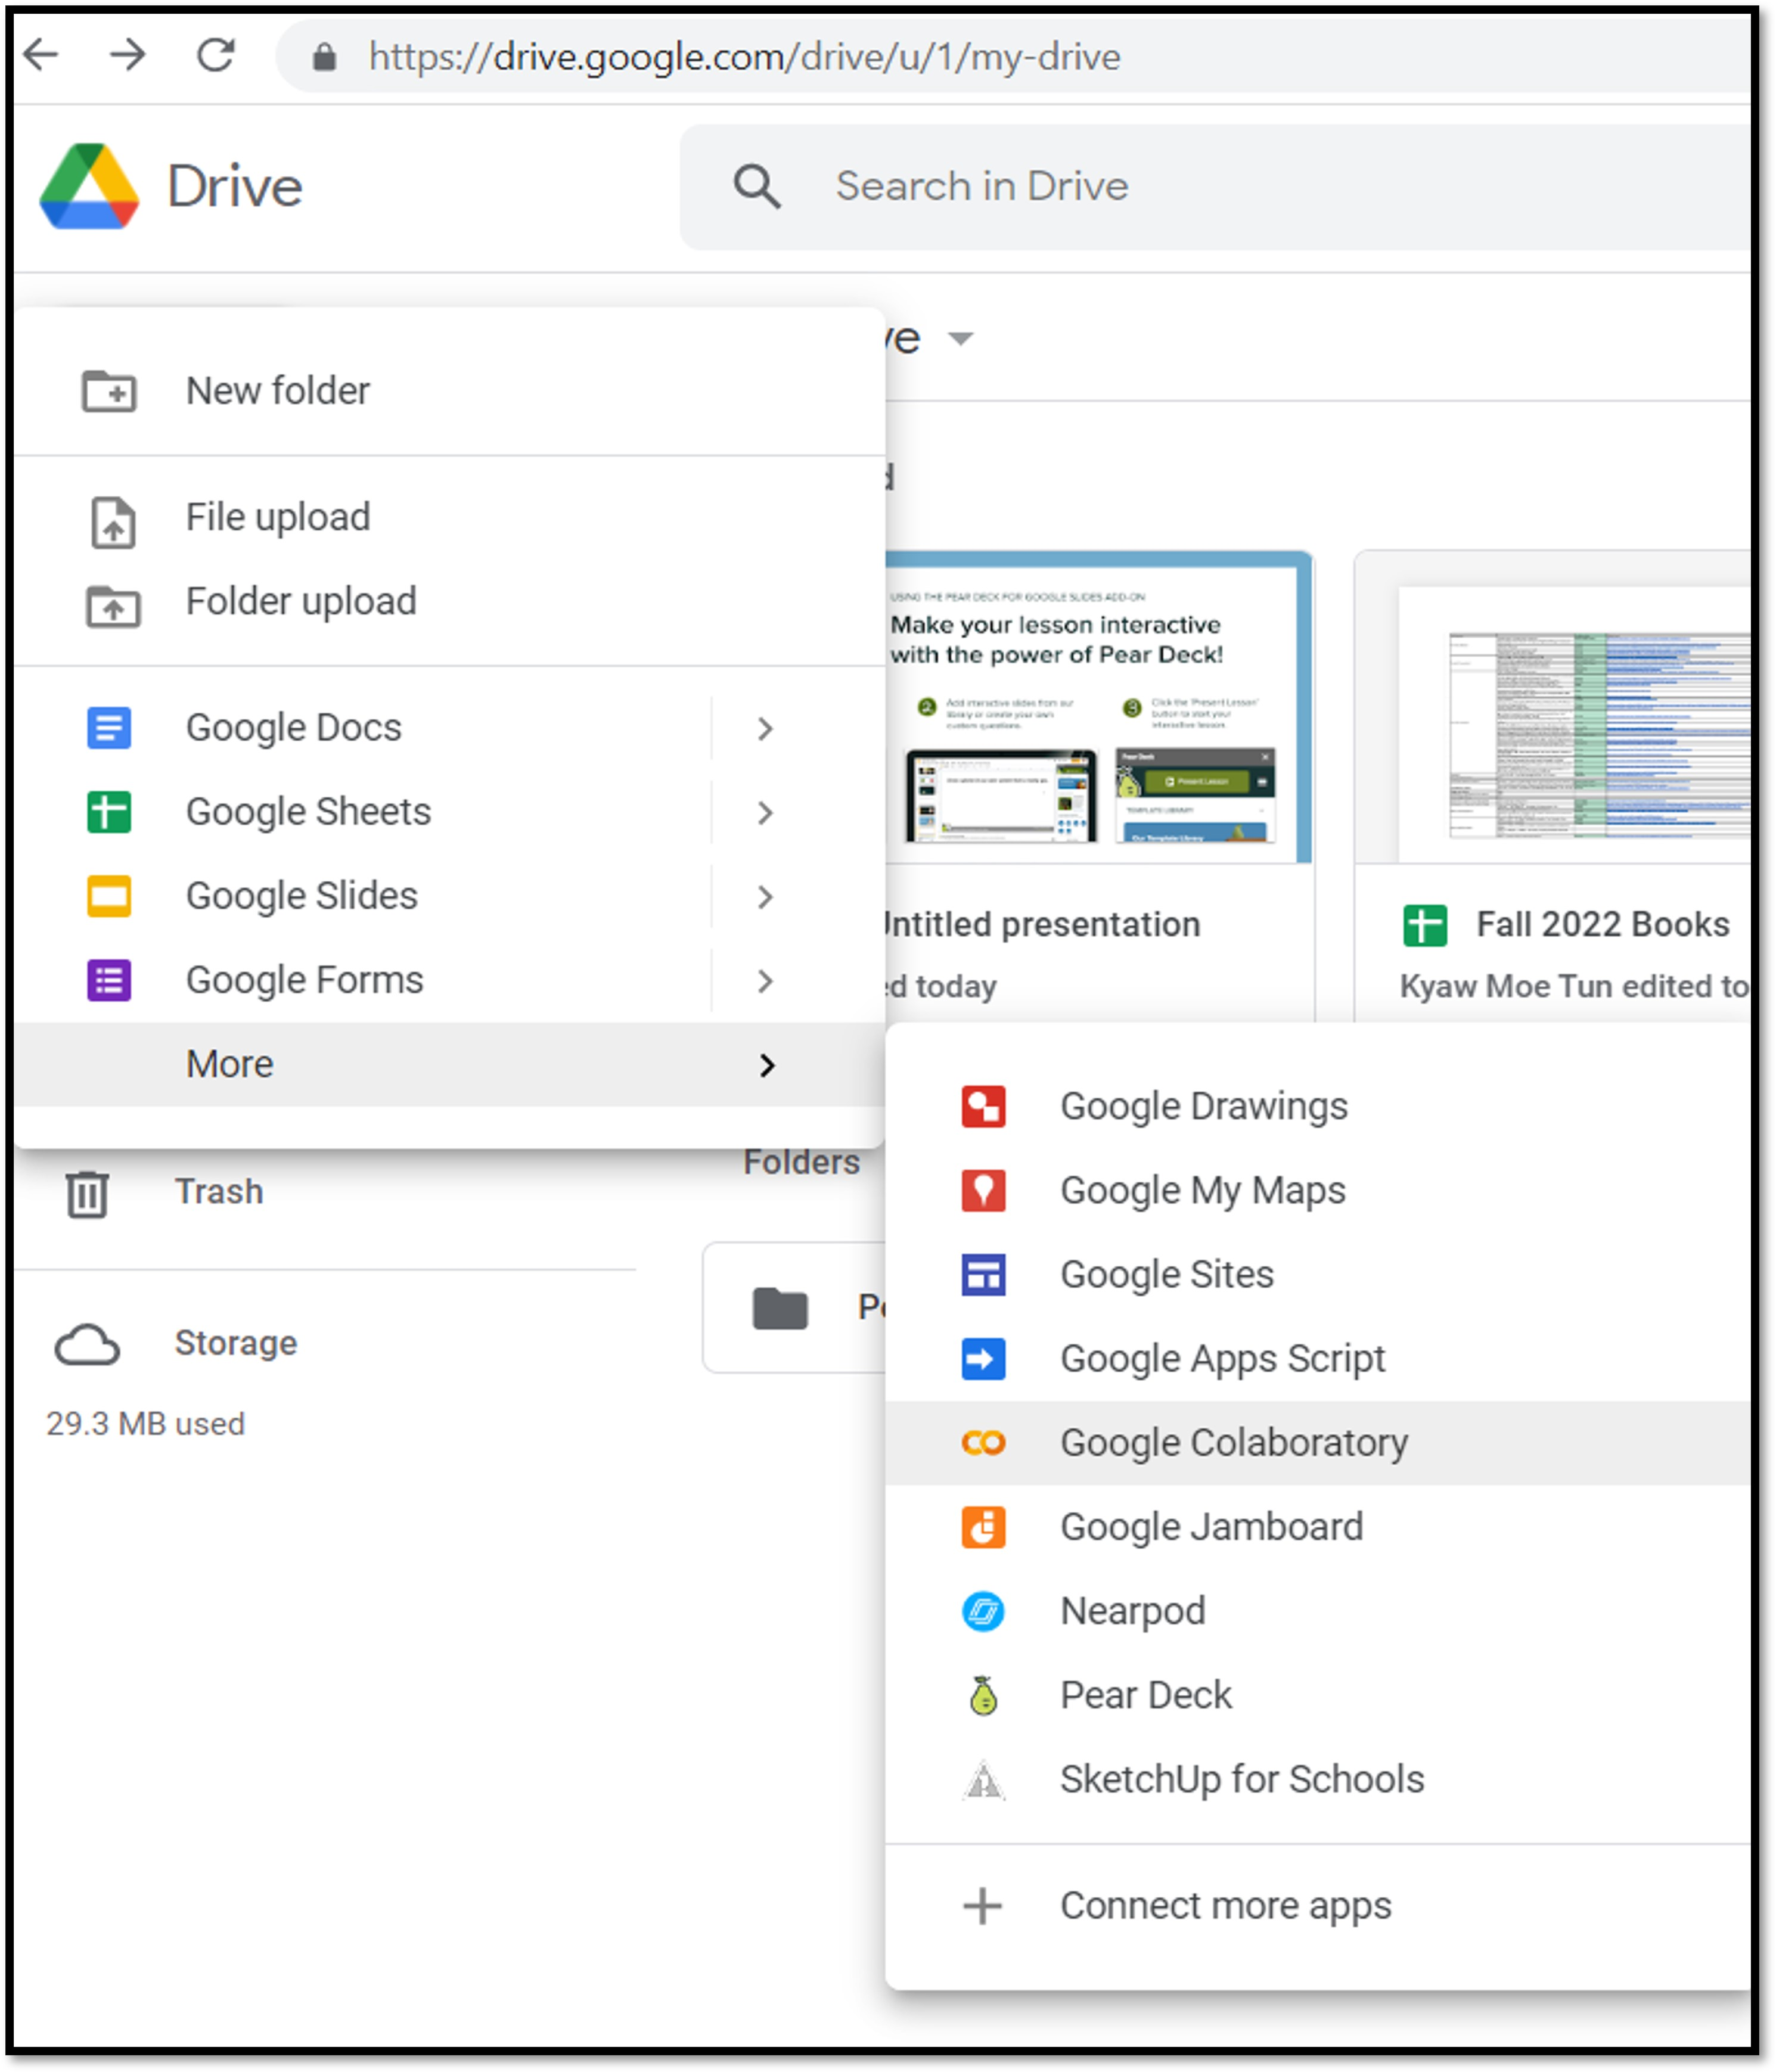
\includegraphics[width=5 cm]{colab1.jpg}
  \caption{Creating a new Colab notebook}
  \label{fig:colab1}
  \end{figure}
   \begin{figure}[!h]
  \centering
  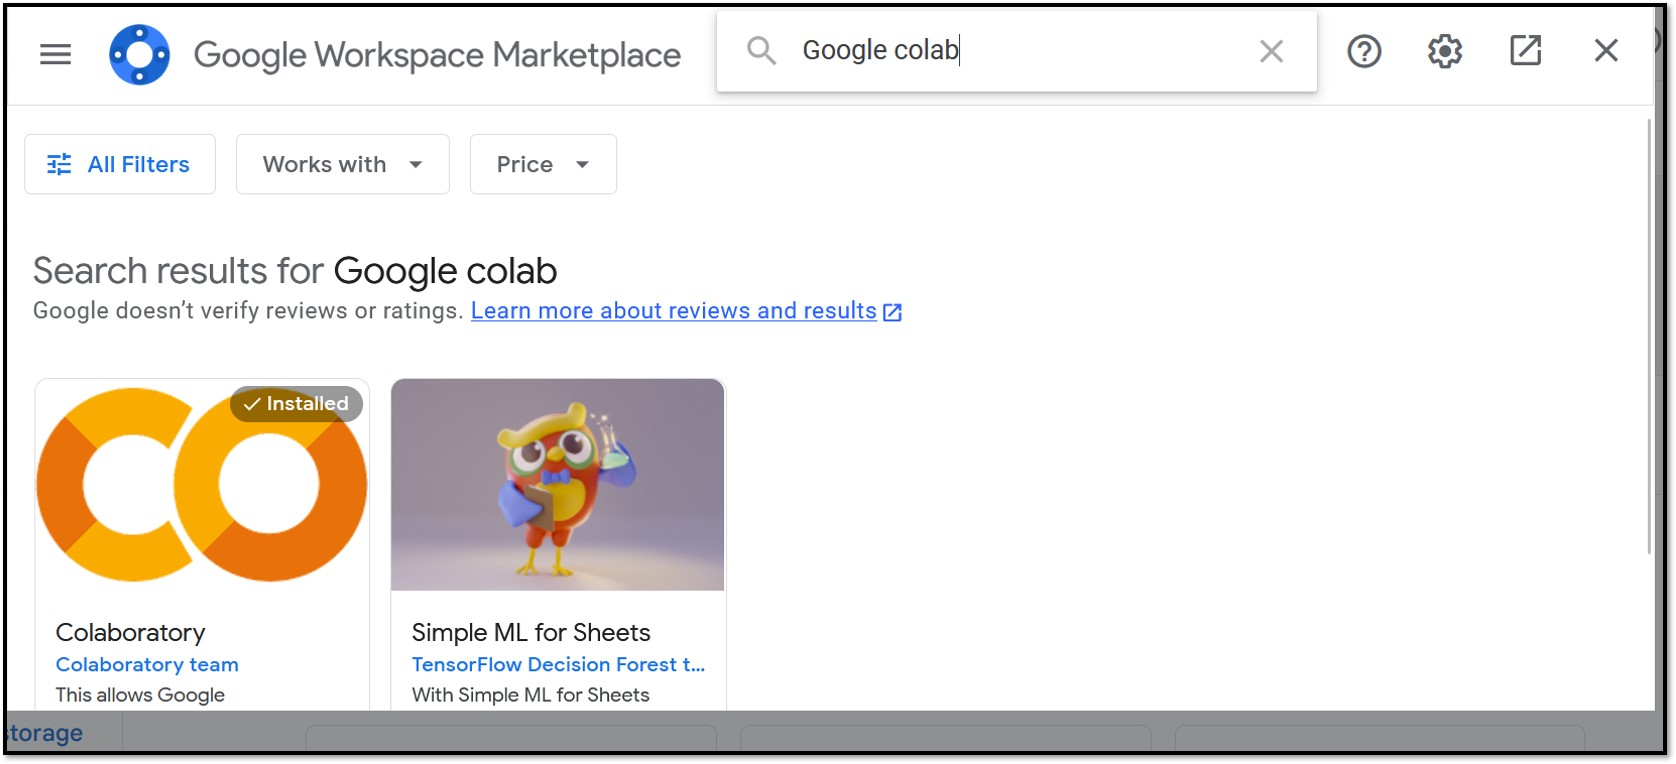
\includegraphics[width=4.5 cm]{colab2.jpg}
  \caption{Connecting to Google Colab App}
  \label{fig:colab2}
  \end{figure}
  \item If you do not find the \emph{Google Colaboratory} in the list, you can click \emph{'Connect more apps'} and search 'Google Colab' in the search bar and add Google Colab to your list as shown in Figure \ref{fig:colab2}.
\end{itemize}
\subsubsection{\textbf{Running a Cell}}
 \begin{itemize}
 \item Make sure the runtime is connected. The notebook shows a green check on the top right corner if it is connected.
 \item Enter your code at the cursor as shown in Figure \ref{fig:colab3}.
 \item To Run cell: press Ctrl + Enter
 \item To Run cell and add new cell below: Alt + Enter
 \item To Run cell and goto cell below: Shift + Enter
 \end{itemize}
 \begin{figure}[h]
  \centering
  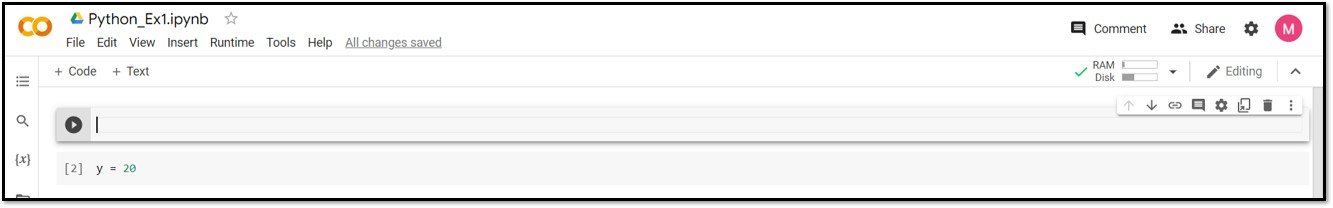
\includegraphics[width=8 cm]{colab3.jpg}
  \caption{Running a cell}
  \label{fig:colab3}
\end{figure}
\newpage
\subsubsection{\textbf{Example Code}}
Figure \ref{fig:import} shows how to read a data file in the Google Colab. Make sure that the files are uploaded into the runtime environment as shown in Figure.
 \begin{figure}[h]
  \centering
  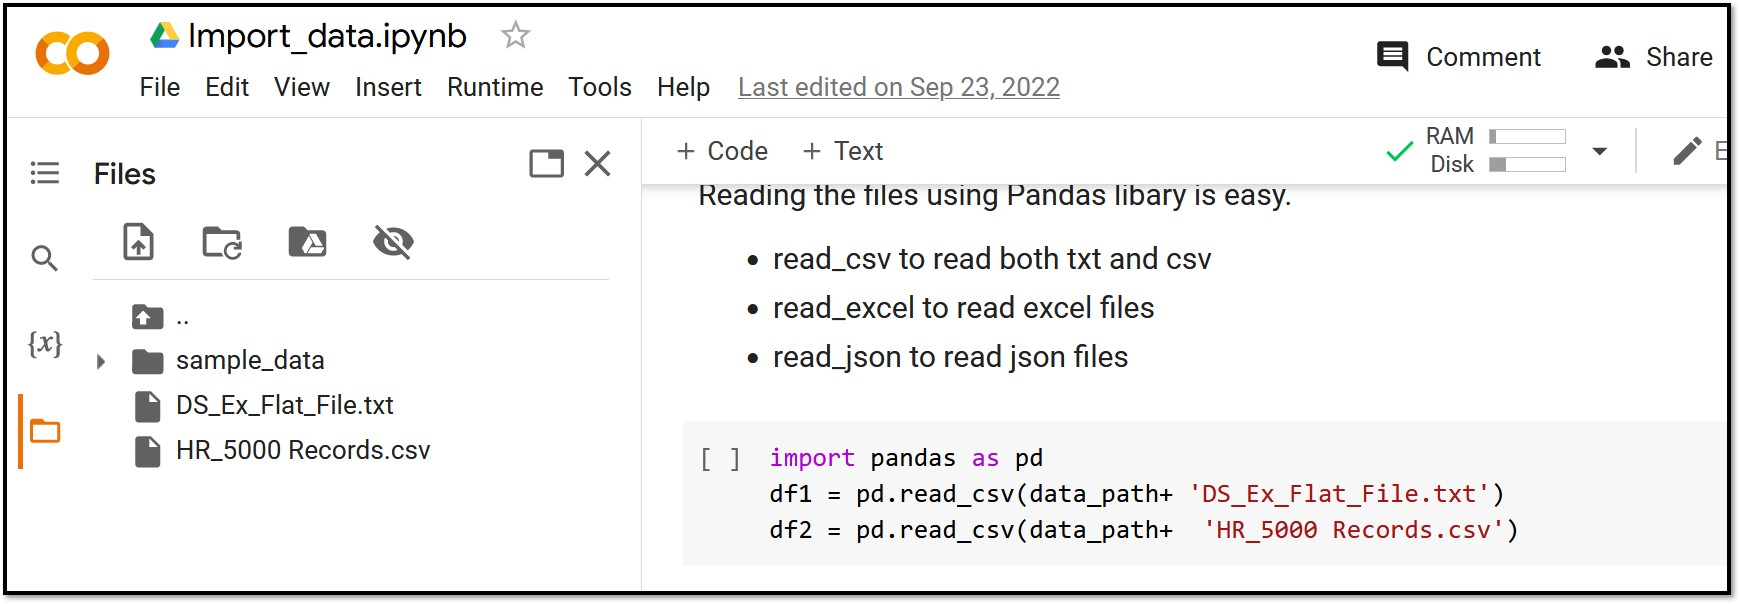
\includegraphics[width=8 cm]{import.jpg}
  \caption{Importing Files}
  \label{fig:import}
\end{figure}
\newpage
\section{Knowledge Test}
\subsection{Supervised or Unsupervised?}
\small{
\begin{questions} %<--- start option fixes number for first question
\question Method to classify if a new patient is having diabetes or not.\\
\begin{oneparchoices}
 \choice  Supervised
 \choice  Unsupervised
\end{oneparchoices}
\question Method to cluster a set of articles into different groups based on similar stories. \\
\begin{oneparchoices}
 \choice  Supervised
 \choice  Unsupervised
\end{oneparchoices}
\question Method to Filter if an email is spam. \\
\begin{oneparchoices}
 \choice  Supervised
 \choice  Unsupervised
\end{oneparchoices}
\question Speech recognition and facial recognition software.\\
\begin{oneparchoices}
 \choice  Supervised
 \choice  Unsupervised
\end{oneparchoices}
\question Segment customer data into groups in marketing environments.\\
\begin{oneparchoices}
 \choice  Supervised
 \choice  Unsupervised
\end{oneparchoices}
\question Detect a fighting event from the CCTV camera.
\begin{oneparchoices}
 \choice  Supervised
 \choice  Unsupervised
\end{oneparchoices}
\end{questions}
}

\subsection{Regression, Classification or Clustering}
\small{
\begin{questions} %<--- start option fixes number for first question
\question Perform initial exploratory analysis on a raw data-set to understand the grouping of data points.\\
\begin{oneparchoices}
 \choice  Regression
 \choice  Classification
 \choice  Clustering
\end{oneparchoices}
\question Method to predict the score of a basketball game. \\
\begin{oneparchoices}
 \choice  Regression
 \choice  Classification
 \choice  Clustering
\end{oneparchoices}
\question You run an online business and you want to predict how many of soft toys will sell over the next month.\\
\begin{oneparchoices}
 \choice  Regression
 \choice  Classification
 \choice  Clustering
\end{oneparchoices}
\question You want to develop an algorithm to check the type of coins (10 baht, 5 baht , 2 or 1 baht).\\
\begin{oneparchoices}
 \choice  Regression
 \choice  Classification
 \choice  Clustering
\end{oneparchoices}
\question Determining whether or not someone will be a defaulter of the loan.\\
\begin{oneparchoices}
 \choice  Regression
 \choice  Classification
 \choice  Clustering
\end{oneparchoices}
\question You run an online shop. You want to group the items sold the most in different seasons.\\
\begin{oneparchoices}
 \choice  Regression
 \choice  Classification
 \choice  Clustering
\end{oneparchoices}
\end{questions}
}


%----------------------------------------------------------------------------------------
%	CHAPTER TWO
%----------------------------------------------------------------------------------------

\chapter{Regression}
As seen in the previous examples, regression analysis uses pre-existing data to understand the relationship between input features and the desired output. In regression analysis, there are five key terms that it's important to be familiar with.

\begin{itemize}
  \item The term \textbf{"Training data"} refers to the pre-existing data that includes the values of the desired output and the input features that affect the output.
  \item The term \textbf{"Target Variable"} refers to the feature of interest. In weather prediction, for example, the temperature would be the target variable. This variable is also sometimes referred to as the "dependent variable" because it is dependent on other variables.
  \item \textbf{"Independent Variables"} are those that are related to the target variable. The target variable often depends on multiple features, but each feature can have a different impact on the target variable. For example, in the case of temperature prediction, factors such as season, time, and regional geography all play a role, but each feature has a different level of influence on the temperature.
  \item \textbf{"Parameters}" refers to the coefficients that determine the relationship between the target variable and independent variables. Training a machine learning model involves identifying these parameters. The number of parameters depends on the complexity of the model.
  \item \textbf{"Residuals"}, also known as errors, refer to the discrepancy between the predicted and actual values.
\end{itemize}

Consider a retail company that utilizes Facebook ads to promote their products. The company wants to determine the effect of increasing their ad spending on their sales volume. In this example, the sales volume is the target variable ($y$) and the spending amount ($x$) is an independent feature. To examine the correlation between sales volume and spending amount, we first need to gather training data on past spending and sales. The relationship between spending and sales can be modeled using a linear equation $y = \omega_1 x + b$ or a polynomial equation $ y = \omega_1 x^k + \omega_2 x^{k-1} + \omega_3 x^{k-2}+ .. + b$. The goal of the machine learning model is to find the coefficients (parameters) that minimize the residual values (the difference between the actual and predicted values).

\newpage
\section{Linear Regression}

Linear Regression is a type of machine learning model that uses a linear equation to predict a target variable based on one or more independent variables. The goal is to find the best parameters that minimize the difference between the predicted and actual values.

It is a simple and widely used method, and can be further divided into simple and multiple linear regression based on the number of variables used.

\subsection{Simple Linear Regression}

Simple Linear Regression is a type of Linear Regression which models the relationship between one independent variable ($x$) and the target variable ($y$) using a linear equation as follow:
\begin{equation}\label{eq:lrmodel}
  y = \omega_1 x + b,
\end{equation} where the coefficient $\omega_1$ and cut off point $b$ are parameters that determine the linear equation used to model the relationship between the target and independent variable. Changing these parameters $\omega_1$ and $b$ results in different models that can describe the relationship between the target $y$ and independent variable $x$. For instance, using the $x$ and $y$ values in Table \ref{tb:lrmodel}, various linear equations can be formulated as below:
\begin{eqnarray}
% \nonumber to remove numbering (before each equation)
  y &=& 100x \\
  y &=& 100x + 800 \\
  y &=& 150x + 800 \\
  y &=& 125x + 800
\end{eqnarray}

\begin{table}[!ht]
\centering
\begin{tabular}{|c|c|c|c|c|c| }
  \hline
  $x$ & 0 & 1 & 2 & 3 & 4  \\
  \hline
  $y$ & 800 & 900& 100 & 1150 & 1300\\
  \hline
\end{tabular}
\caption{Example values of the target and the independent variable.}\label{tb:lrmodel}
\end{table}

The goal of a Simple Linear Regression model is to find the optimal parameters ($\omega_1$ and $b$) that can accurately predict the target variable ($y$)  for a new independent variable ($x$).

\begin{figure}[!h]
  \centering
  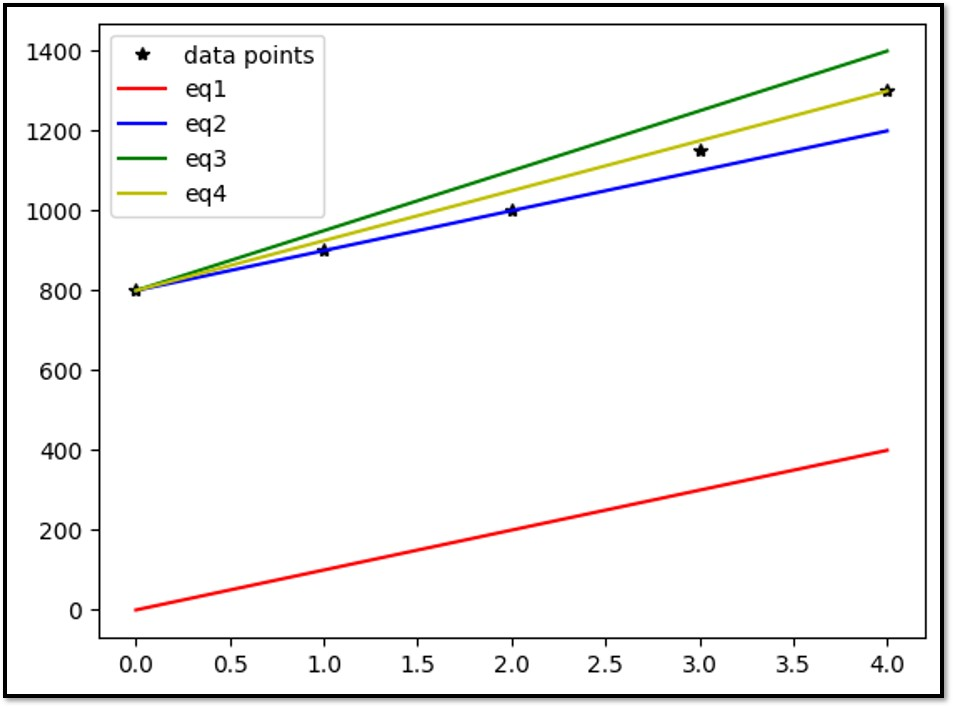
\includegraphics[width=8.2 cm]{LRmodel.jpg}
  \caption{An example of a Linear Regression Model}
  \label{fig:LRmodel}
\end{figure}

Figure \ref{fig:LRmodel} illustrates the data and the lines generated by the four different equations (2.2 to 2.5). The black stars represent the training data points listed in Table 2.1. It's clear that the red line does not fit the data points well and is not a good model. The yellow and blue lines pass through some of the data points. The goal of Simple Linear Regression is to find the parameters that produce a line that best describes the relationship between the target variable $y$ and independent variable $x$. The best model is the one that results in the least difference between the actual and predicted values.

\subsubsection{\textbf{Cost Function}}

The cost function is a measure of the average squared error (or residual) between the actual and predicted values. Mathematically,
\begin{equation}\label{eq:cost}
  \varepsilon = \frac{1}{N}\sum_{i=1}^N (\tilde{y_i}-y_i)^2,
\end{equation} where $N$ represents the number of data points (or observations) and $\tilde{y_i}$ represents the predicted value using the model, which can be described as:
\begin{equation}\label{eq:ypred}
   \tilde{y_i} = \omega_1 x_i + b,
\end{equation}where $\omega_1$ and $b$ are model parameters.

\newpage
\subsection{Multiple Linear Regression}
Multiple Linear Regression is an extension of Simple Linear Regression that takes into account more than one independent variable to predict the target value. This is achieved by using a linear equation, and it can be mathematically represented as:

\begin{equation}\label{eq:lrmodel}
  y = \omega_1 x_1 + \omega_2 x_2 + \omega_3 x_3 + ... + b,
\end{equation} where $\omega_i, i =0, 1, 2, ...$ are parameters of the model.

Like in Simple Linear Regression, the objective of Multiple Linear Regression is to find the parameters that minimize the cost function in equation \ref{eq:cost}. However, since it uses more than one feature, the different ranges of values of the features can lead to one feature having more influence than the other in predicting the target value. Therefore, it is essential to scale the features to have the same or similar ranges of values.

\newpage
\subsection{Feature Scaling}
Feature scaling is a technique used to adjust the independent variables to a similar range of values. There are several methods for feature scaling, including min-max scaling and z-score standardization, which are among the most widely used. Min-max scaling is often used in conjunction with neural networks, while z-score standardization is more frequently applied to linear regression models.

\subsubsection{\textbf{Min-Max Scaling}}
Min-max scaling, also referred to as normalization, is a method for scaling data into a range of 0 to 1. It is mathematically defined as:
\begin{equation}\label{eq:normalization}
   x_{scaled} = \frac{x-x_{min}}{x_{max}-x_{min}},
\end{equation}where $x_{min}$ and $x_{max}$ represent the minimum and maximum values of the variable $x$. The minimum value of $x$ will be mapped to 0 and the maximum value to 1, and all other values of $x$ will be scaled accordingly.

\newpage

\subsubsection{\textbf{Z-score Standardization}}
Z-score standardization, also known as zero-mean scaling, is a method that scales the values of each independent variable to have a mean of zero and a standard deviation of one. It can be calculated using the following formula:

\begin{equation}\label{eq:standardization}
   x_{scaled} = \frac{x-\mu}{\sigma},
\end{equation}where $\mu$ and $\sigma$ are mean and standard deviation of the variable $x$.

\newpage
\subsection{Assumptions}
There are four underlying assumptions in linear regression methods:
\begin{enumerate}
  \item \textbf{Linear relationship}: There should be a linear relationship between the target $y$ and independent variables $x_i$. This means that a change in $y$ due to a unit change in $x$  should be constant. If the relationship is not linear, the linear regression may not predict the target values correctly.
  \item \textbf{No multi-collinearity}: The independent variables should not be correlated, otherwise it becomes difficult to identify how they individually influence the target value and it can inflate the standard errors of some or all of the regression coefficients.
  \item \textbf{Consistent variance of residuals}: The variance of the residuals should be consistent across all predicted values, otherwise the estimates for the model coefficients may become unreliable.
  \item \textbf{Normally distributed residuals}: The residuals should be normally distributed, meaning most of the data points should be close to one straight line and the points farther away should fall off smoothly and symmetrically. If this is not the case, linear regression may not be a good choice for the problem.
\end{enumerate}

It is important to check if these assumptions are met when considering linear regression for modeling and deploying.

\newpage
\subsection{Knowledge Test}
\small{
\begin{questions} %<--- start option fixes number for first question
\question Table \ref{tb:lrmodel} shows the income earned by Mr 'Arm' based on the number of overtime hours he worked. Represent the relationship between the overtime hours and income using the equation $y=ax+b$ where $x$ represents overtime hours and $y$ represents income. Find the values of `a` and `b` and chose the best equation. Explain your reasoning for the chosen equation.
\begin{itemize}
  \item $y = 100 x + 800$
  \item $y = 125 x + 800$
  \item $y = 150 x + 800$
\end{itemize}
\question Why is feature scaling important in multiple linear regression?

\question What is the assumption of linearity in linear regression?

\question What is multi-correlation and why is it important to avoid in linear regression?

\question Can you explain the normality assumption in linear regression?

\question The multiple linear regression model for predicting sale volume is represented as $ y = 3.92 x_1 + 2.79 x_2 + 0.01x_3 + 14$ where $y$  is the sale volume, $x_1$  is the amount spent on TV advertising, $x_2$ is the amount spent on radio advertising, and $x_3$ is the amount spent on newspaper advertising.
\begin{enumerate}
  \item Which advertisement program has the least impact on sale volume? Can you explain your reasoning?
  \item If we increase the amount spent on TV advertising by one dollar while keeping the other two programs constant, what will be the resulting sale volume? Can you explain your reasoning?
\end{enumerate}

\end{questions}

\newpage
\section{Gradient Descent Method}\label{sec:GDS}
The Gradient Descent method is an optimization algorithm that finds the values of parameters (coefficients) that minimize a cost function. In the context of simple linear regression, the cost function depends on two parameters ($\omega_1$ and $b$) and can be represented in terms of the parameter $\theta$ as:

\begin{equation}\label{eq:costGDS}
  J(\theta) = \frac{1}{N} \sum_{i=1}^N \left((\omega_1 x_i + b) - y_i\right)^2,
\end{equation} where $\theta \in (\omega_1, b)$. To find the minimum of this function, we first compute the gradient, which measures the change in all weights in relation to the change in error. The changes of $J(\theta)$ with respect to $\omega_1$ and $b$ are given below as:

\begin{eqnarray}
  \frac{\partial J(\theta)}{\partial \omega_1} &=& \frac{2x_i}{N} \sum_{i=1}^N \left((\omega_1 x_i + b) - y_i\right)\\
  \frac{\partial J(\theta)}{\partial b} &=& \frac{2}{N} \sum_{i=1}^N \left((\omega_1 x_i + b) - y_i\right)
\end{eqnarray}

\newpage
\noindent The implementation of the Gradient Descent method can be broken down into four steps:

\begin{description}
  \item[Step 1] Initialize the parameters $\theta_k$.
  \item[Step 2] Compute the cost function value $J_k(\theta)$ using the parameters $\theta_k$.
  \item[Step 3] Update the parameters :
  \begin{equation}
  \theta_{k+1} = \theta_k - \alpha \frac{d J(\theta)}{d\theta}
  \end{equation} where the parameter $\alpha$ is a learning rate.
  \item[Step 4] Repeat steps 2 and 3 until the changes in cost function values are very small, or for a pre-defined number of iterations.
\end{description}

The performance of gradient descent is affected by the initial values of the parameters and the size of the learning rate. A high learning rate may prevent the algorithm from finding the local minimum and reaching the best solution, while a low learning rate may extend the time needed for the algorithm to reach convergence.

\begin{figure}[!h]
  \centering
  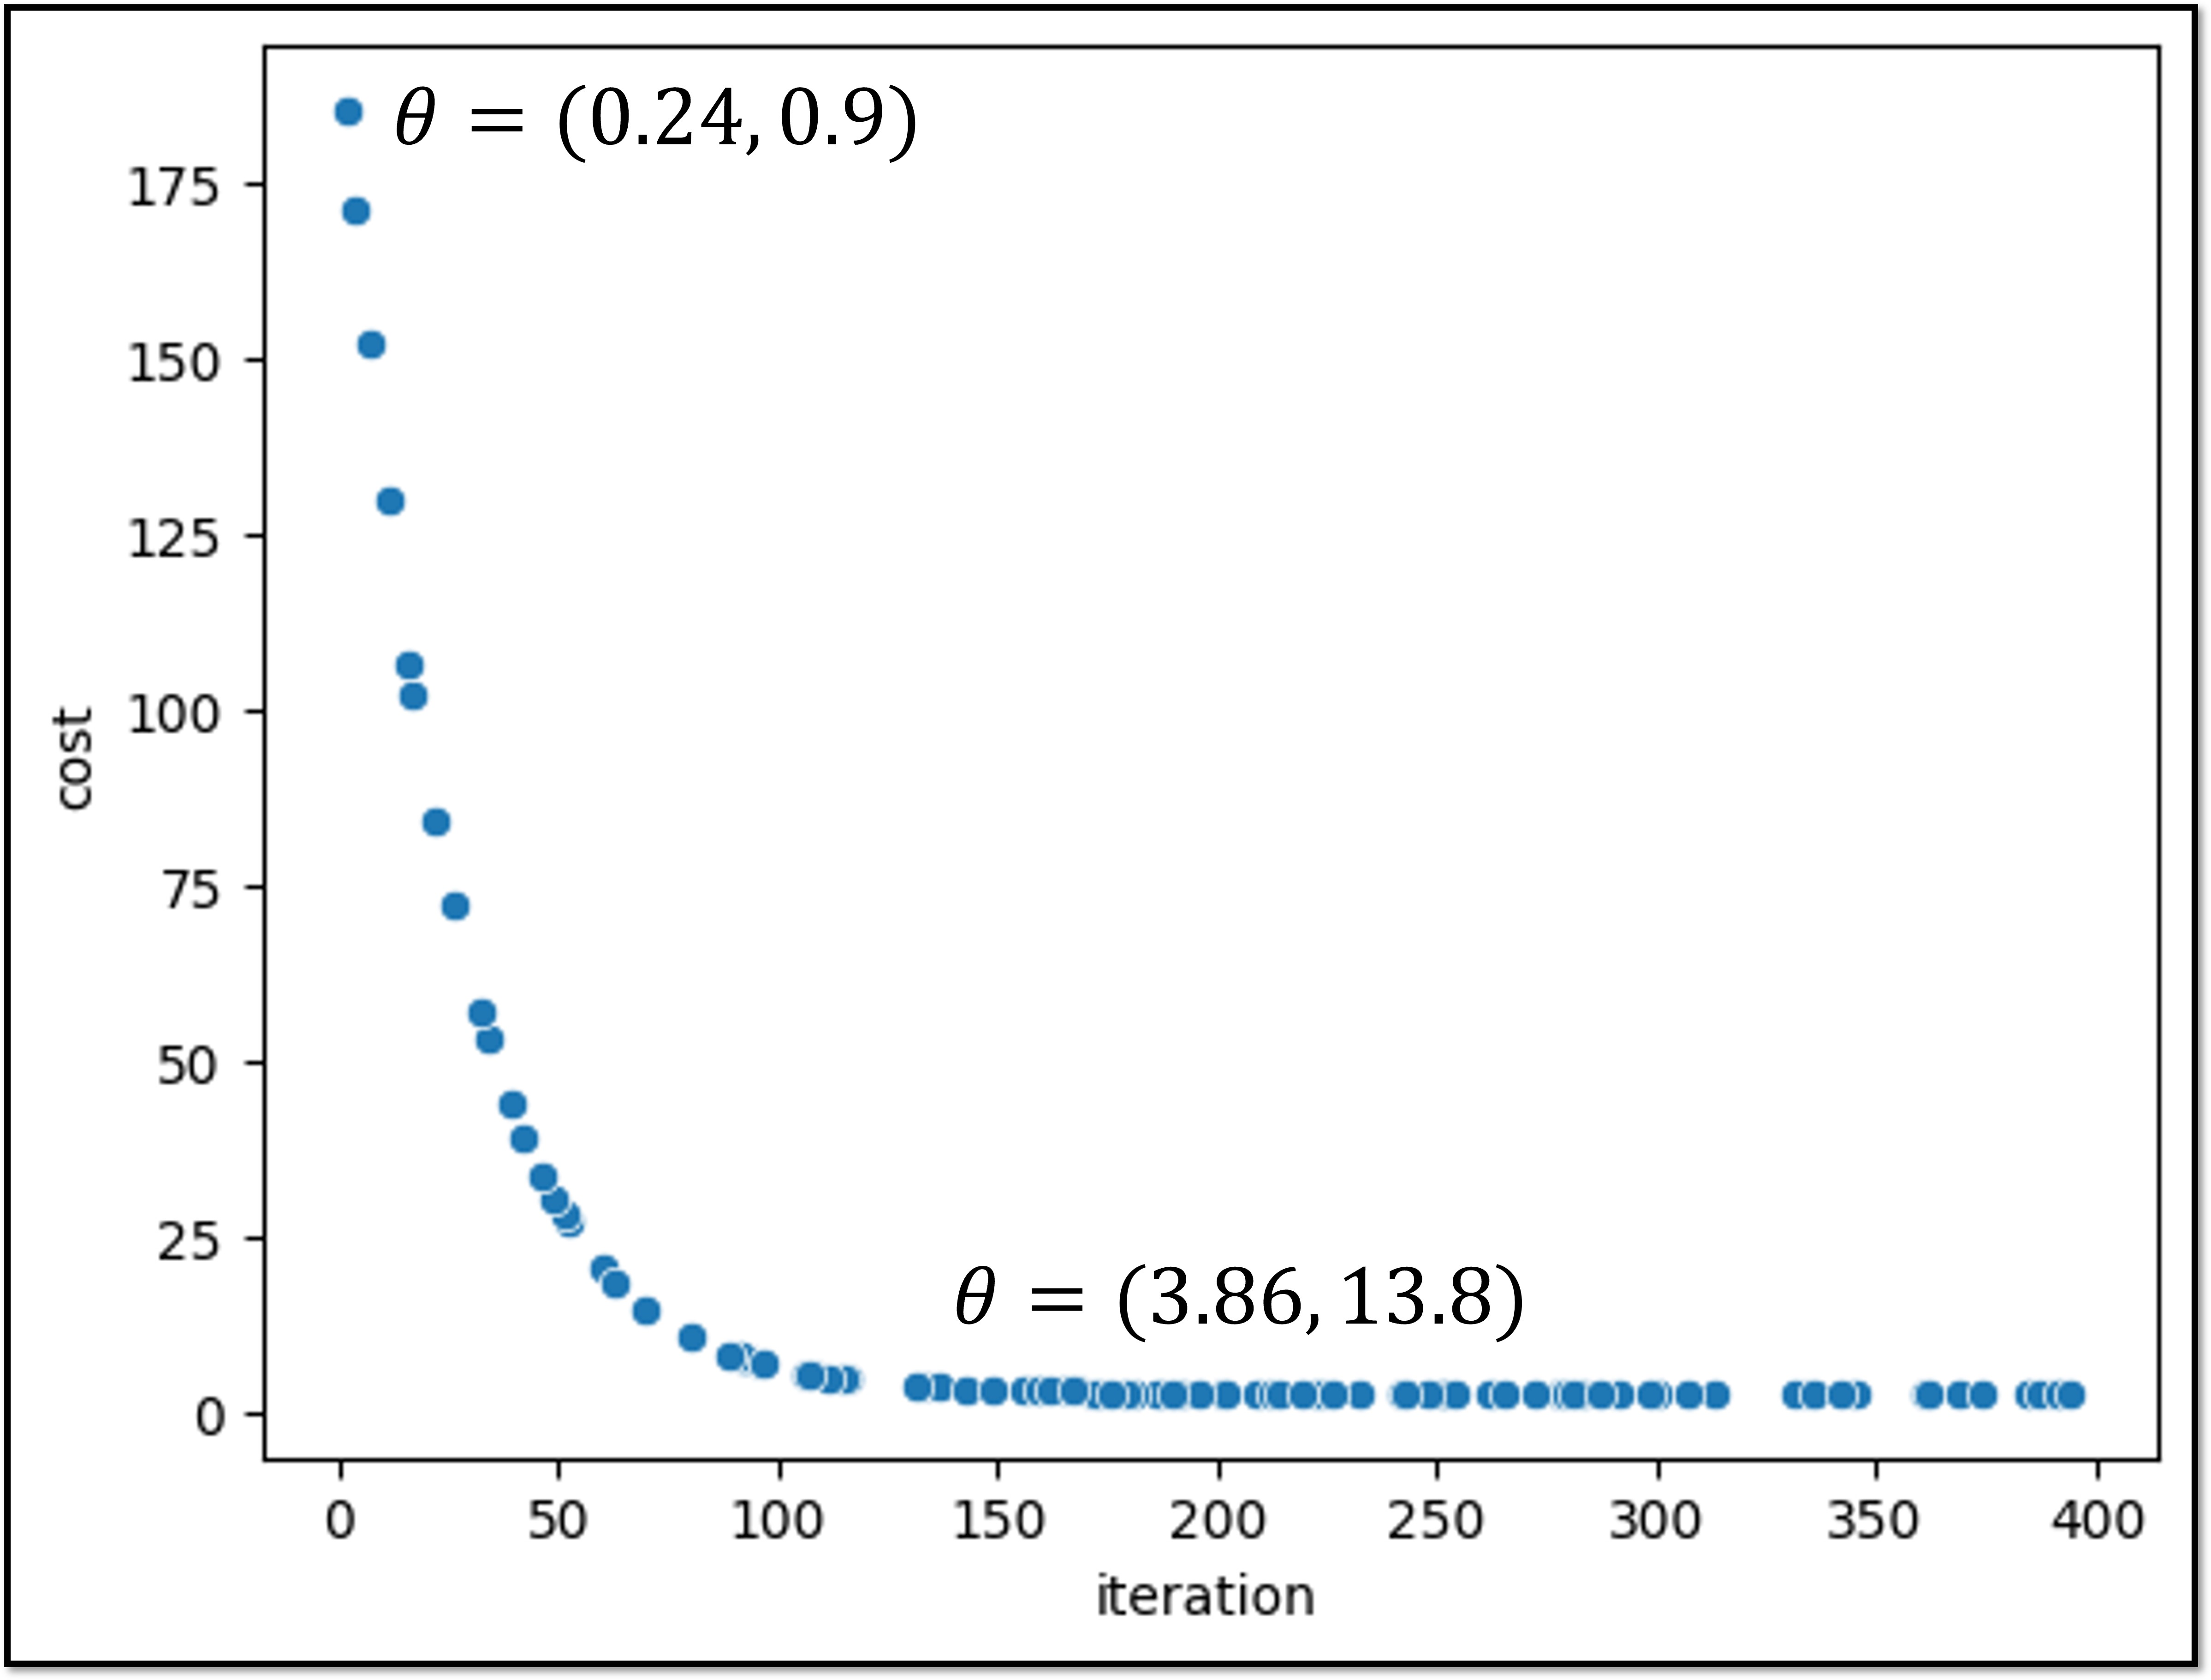
\includegraphics[width=7.5 cm]{gds_rate.jpg}
  \caption{How does the Gradient Decent Method work?}
  \label{fig:gdsRate}
\end{figure}

Figure \ref{fig:gdsRate} illustrates the operation of the gradient descent method. The parameter, $\omega_1$ and $b$ are initially set to $0.24$ and $0.9$ respectively. The gradient descent method then repeatedly modifies the parameters until the cost function reaches convergence. In this example, the cost function reaches a minimum value of $2.85$ at iteration 200, when the values of the parameters are $\omega_1 = 3.86$ and $b = 13.8$. Beyond iteration 200, the cost function does not change significantly, indicating that these values of the parameters provide the optimal solution with the smallest difference between the actual and predicted values.

\subsection{Knowledge Test}

\begin{questions}

\question Can you explain the concept of the learning rate in the gradient descent method?

\question What is the effect of feature scaling on the gradient descent method?

\question Figure \ref{fig:gdsRate} shows the values of cost function resulted by running gradient descent for 400 iterations with $\alpha =0.01$. The graph shows that the cost function, $J(\theta)$ decreases rapidly at first and then levels off.
\begin{itemize}
  \item what do you think will happen to the cost function if the learning rate is increased to 1 ($\alpha =1$)?
  \item what do you think will happen to the cost function if we decrease the value of the learning rate to 0.001 ($\alpha =0.001$)?
\end{itemize}

\end{questions}

\newpage

\section{Polynomial Regression}
A polynomial regression model represents the association between a target variable and one or more independent variables by means of an equation of the $n^{th}$ degree polynomial equation. When there is only one independent variable, $x$, the model can be formulated as

\begin{equation}\label{eq:polyEq}
  y = \omega_1 x^n + \omega_2 x^{n-1} + \omega_3 x^{n-2} + ... + \omega_n x + b
\end{equation} where $b$ is the cut off point, and $\omega_i$ where $i$ ranges from $1$ to $n$ are coefficients of the independent variable.


\begin{figure}[!ht]
  \centering
  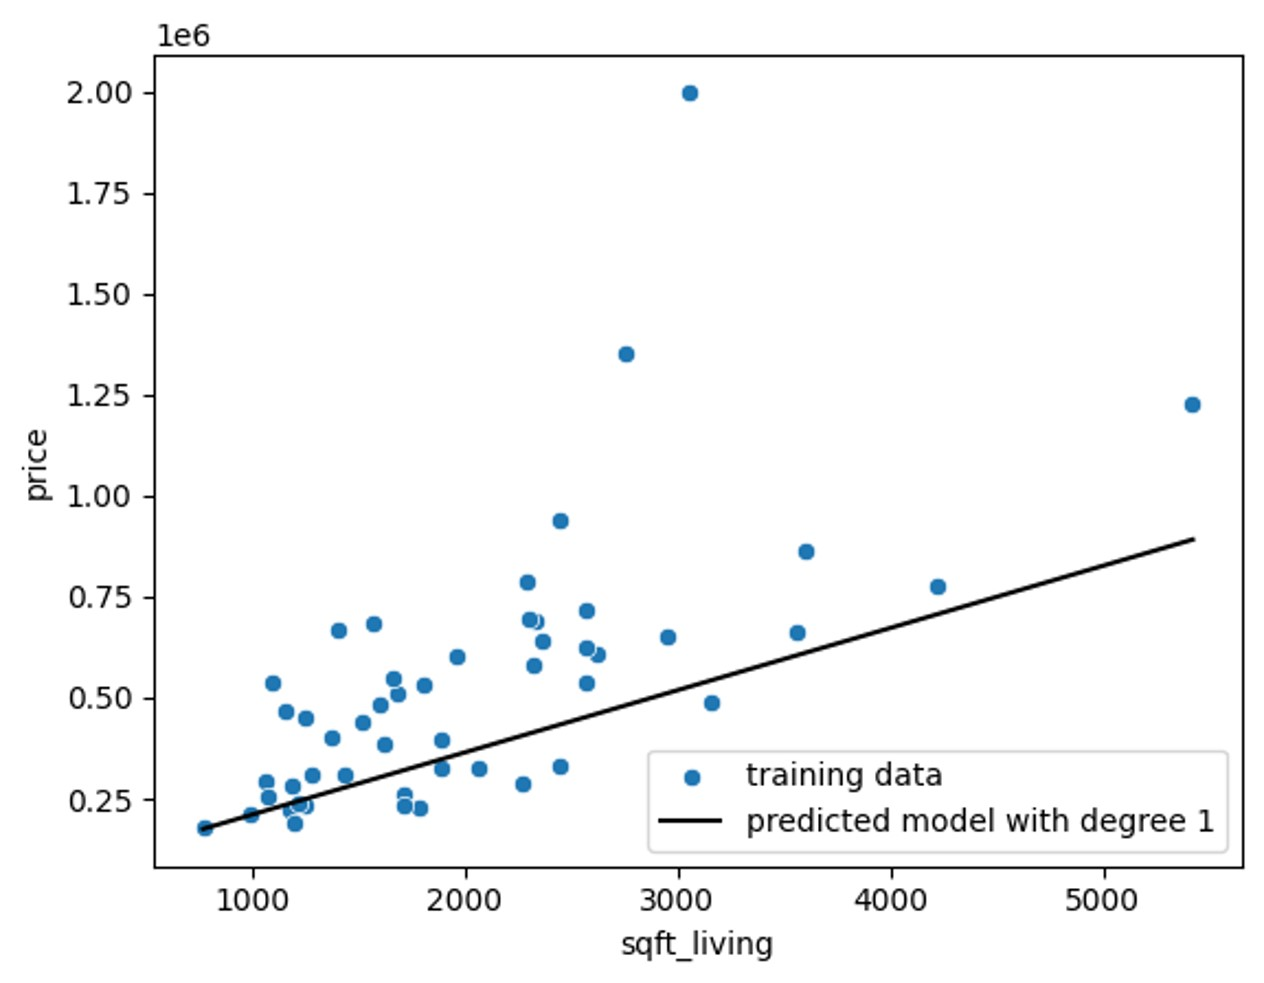
\includegraphics[width=4 cm]{poly_demo1.jpg}
  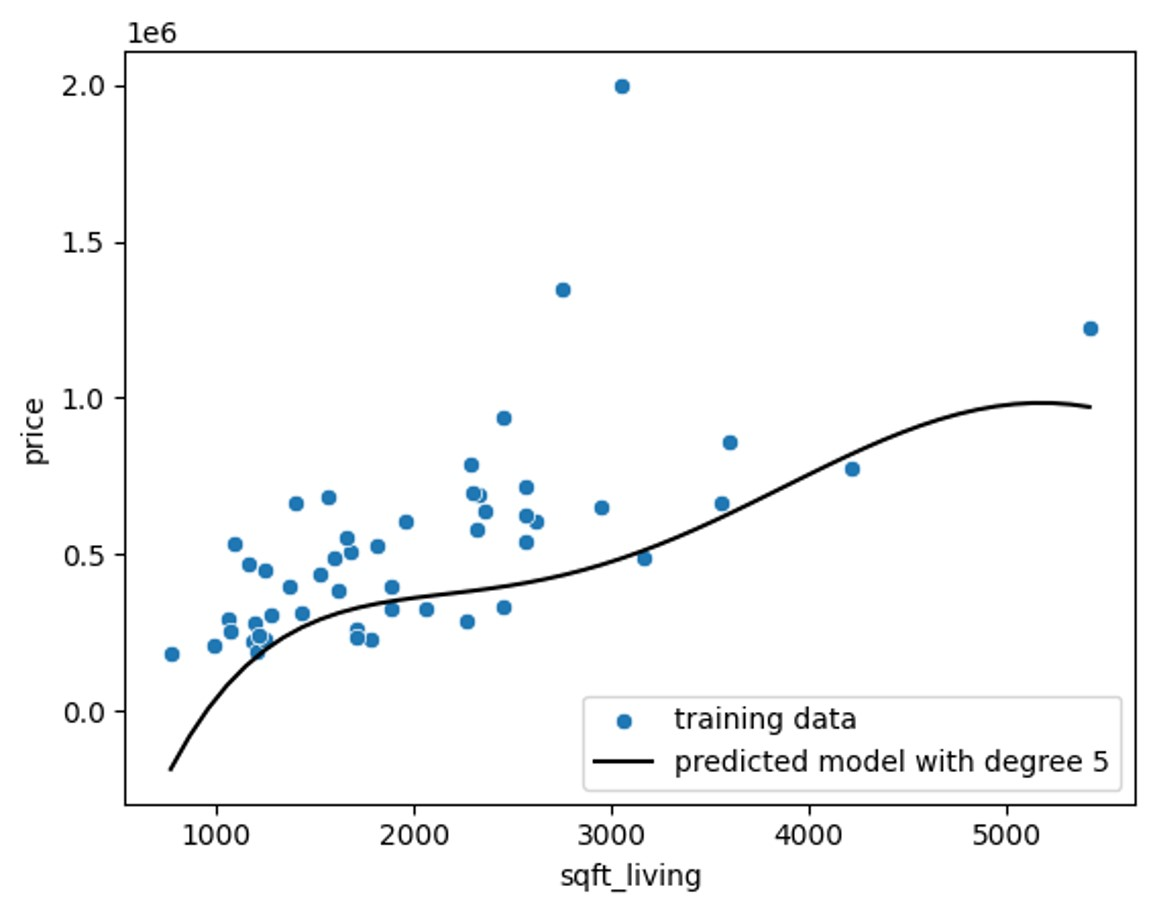
\includegraphics[width=4 cm]{poly_demo2.jpg}
  \caption{Linear Regression vs. Polynomial Regression}
  \label{fig:polydemo}
\end{figure}

Figure \ref{fig:polydemo} illustrates the difference between linear and polynomial regression when using a single feature. Polynomial regression uses a curve to fit the data, while linear regression uses a straight line. As the degree of the polynomial increases, the fit of the curve to the data improves and the difference between actual and predicted values decreases. In general, when the relationship between the target and independent variables is non-linear and cannot be represented by a straight line, polynomial regression tends to provide a better fit than linear regression.

However, using a higher degree polynomial also increases the number of parameters and makes the computation more complex. For a single feature, the number of parameters for an $n^{th}$ degree polynomial is $n+1$, and it would be even higher for multiple features.
\newpage
\subsection{Multiple Features}
The mathematical equation for a 2nd-order polynomial regression model with 2 independent variables is as follows:

\begin{eqnarray}\label{eq:MpolyEq}
% \nonumber % Remove numbering (before each equation)
\nonumber  y &=& \omega_1 x_1^2 + \omega_2 x_1 + \omega_3 x_2^2 + \omega_4 x_2 \\
             &+& \omega_5 x_1 x_2 + b
\end{eqnarray} A $2^{nd}$-order polynomial regression model with 4 features has 5 coefficients and one association and one cut-off point. As the polynomial degree and number of features increase, the number of coefficients also increases.

\newpage
\subsection{Implementation}
In contrast to linear regression methods, using polynomial regression requires an additional step, as illustrated in Figure \ref{fig:polyImple}. The data must be transformed to a higher dimensional space in order to model the relationship between the target and independent variables using a linear equation. Then, the parameters can be determined using the Gradient descent method, as previously described in section \ref{sec:GDS}.

\begin{figure}[!ht]
  \centering
  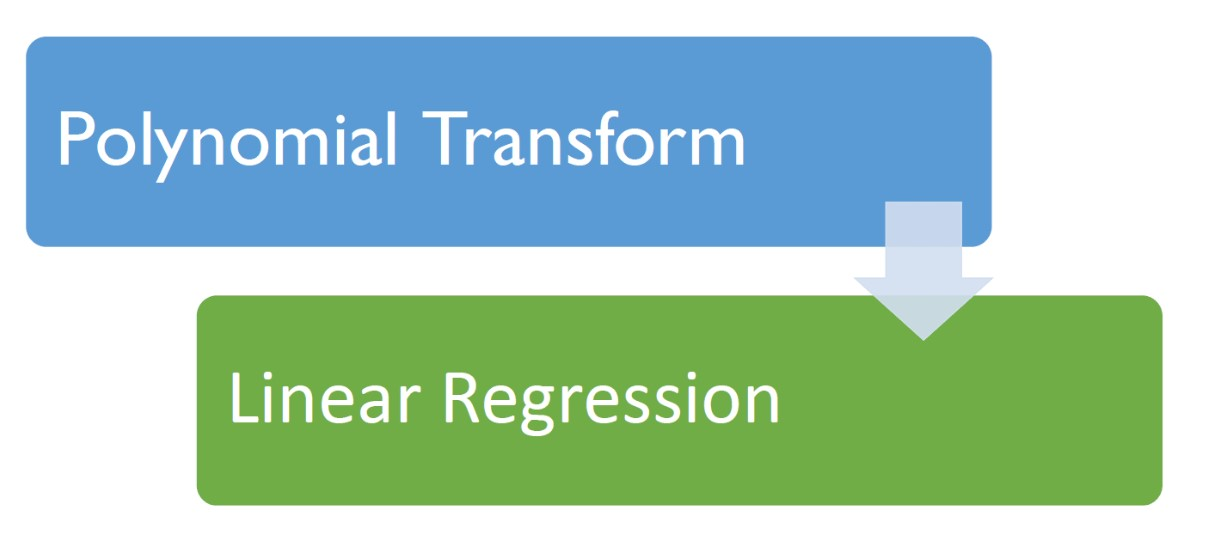
\includegraphics[width=6 cm]{poly_transform.jpg}
  \caption{Polynomial Regression Implementation}
  \label{fig:polyImple}
\end{figure}

\newpage
\subsection{Hyper-parameter}
In polynomial regression, the degree of order is a hyper-parameter that must be selected and provided as input to the model. Typically, a higher degree of order will provide a better fit to the data and result in a lower difference between actual and predicted values. However, as the order increases, the model may attempt to fit every single data point in the data-set and lose its ability to generalize to new data, known as over-fitting. The topic of how to prevent over-fitting and choose appropriate hyper-parameters will be discussed in section \ref{sec:hyperP}.

\newpage
\subsection{Knowledge Test}
\begin{questions}

\question How does polynomial regression differ from linear regression?

\begin{figure}[!h]
  \centering
  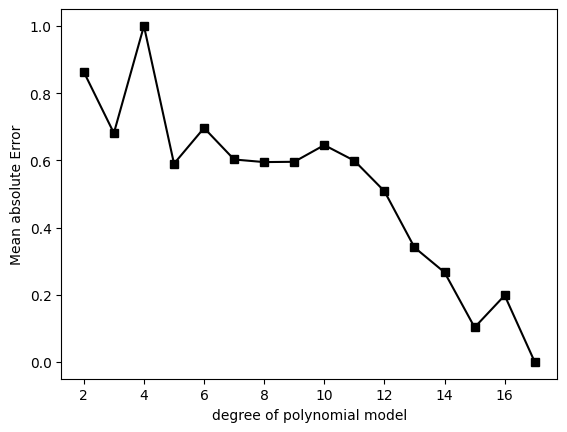
\includegraphics[width=6 cm]{order_poly.png}
  \caption{Mean squared error vs. order of the Polynomial regression Model}
  \label{fig:polyOrder}
\end{figure}

\question Figure \ref{fig:polyOrder} shows the plot of the mean squared error obtained for different order of the polynomial regression model. Which order of the polynomial regression model has the lowest mean squared error? Can you explain why this may or may not be the best choice?
\end{questions}

\newpage

\section{Model Implementation}\label{sec:model}
The implementation of machine learning models has become much simpler and more efficient with the advancement of various python libraries. This section will cover the step-by-step process of implementing a machine learning model using Python.

\subsection{Data Preparation}
Data preparation, also known as data pre-processing, is a necessary step before building any machine learning model. This stage includes:
\begin{itemize}
  \item cleaning the data, such as removing outliers and identifying incorrect or missing information,
  \item analyzing the data to understand the relationship between the target and different features, and detect any correlation among features,
  \item creating new features from the existing features through feature engineering.
\end{itemize}In summary, this stage makes the data suitable for use in the machine learning modeling process.


\newpage
\subsection{Data Splitting: Train-Test Split}
A supervised regression method aims to predict unseen data using a model trained on labeled data. If all of the available data is used to train the model and determine its parameters, the model may perform well on the training data but poorly on unseen data. To ensure the model will perform well on unseen data, it is important to set aside a portion of the data as a testing set.

The process of dividing the labeled data into a training set for model training and a testing set for evaluation is called Train-Test Split. To ensure that the model is accurate, it is crucial to use a sizable training set that captures the underlying correlations in the data, and to randomly select the data for the split to create representative sets. Usually, the standard practice is to use two-thirds of the data for training and the remaining one-third for testing.

\subsubsection{\textbf{Train-Test Split in Python}}
The scikit-learn library in Python makes it easy to perform data splitting using the train\_test$\_$split function from the model$\_$selection module. This function takes a loaded data-set as input and separates it into two subsets. It is a good practice to first separate the independent variables ($X$) and the target variable ($y$) from the labeled data, and then pass $X$ and $y$ to the train$\_$test$\_$split function. This function will randomly split both $X$ and $y$ into training and testing sets.

In the example provided, the data set used is "Advertising.csv" \cite{web:adData}, in which the sale amount is the target variable and depends on the advertisement cost in  \emph{`TV', `radio', and `newspaper'}. The below python codes read the \emph{`Advertising'} data set from the data folder and extract the independent variables ($X$) and the target variable ($y$) from the data-set. Then, the data set is randomly split into 67 percent as training and 33 percent as testing data.

\begin{lstlisting}[language=Python]
# ==================================================#
import pandas as pd
from sklearn.model_selection import train_test_split

df=pd.read_csv('..\\data\Advertising.csv')
X=df[['TV', 'radio', 'newspaper']]
y=df['sales']

X_train, X_test, y_train, y_test = train_test_split(X,y,
                                    test_size = 0.33,
                                    random_state=1)
# ==================================================#
\end{lstlisting}
The random state is set at 1 so that the same subset is provided by Python every time we run the code.

\newpage
\subsection{Data Modelling}
In this stage, a machine learning method is modeled using a training dataset. The section includes discussion and implementation of linear and polynomial regression using Python.

\subsubsection{\textbf{Linear Regression in Python}}
The following code demonstrates how to model linear regression using the Python sklearn library. It is important to note that the $X_{train}$ variable includes multiple features. The code for both simple and multiple linear regression is the same, except for the dimensions of the $X_{train}$ variable. The "\emph{fit}" function under the Linear Regression module finds the optimal parameters that minimize the difference between the actual and predicted values of the target variable, "sale amount."

\begin{lstlisting}[language=Python]
# ==================================================#
from sklearn.linear_model import LinearRegression

lr = LinearRegression()
lr.fit(X_train, y_train)

print(lr.coef_, lr.intercept_)

# ==================================================#
\end{lstlisting}

Feature scaling is a crucial step in building a multiple linear regression model. It can be accomplished by using the pre-processing module in the sklearn library.

The following Python code demonstrates how to perform feature scaling and then use the scaled features to train a linear regression model. By normalizing the features, it can make sure that one feature does not dominate over the other, and all the features are on the same scale, which can help the optimization algorithm converge faster. It can also help to prevent numerical instability and can improve the performance of the model.

\begin{lstlisting}[language=Python]
# ==================================================#
## feature scaling

from sklearn.preprocessing import StandardScaler

scale = StandardScaler()
X_scaled = scale.fit_transform(X_train)
## linear regression model
from sklearn.linear_model import LinearRegression

lr = LinearRegression()
lr.fit(X_scaled, y_train)
print(lr.coef_, lr.intercept_)
# ==================================================#
\end{lstlisting}


\subsubsection{\textbf{Polynomial Regression in Python}}

Polynomial regression is an extension of linear regression that involves a step of feature transformation. The following code demonstrates how to implement polynomial regression using the sklearn library. It is performed by adding polynomial features, which are derived from the original features, to the input data-set, and then fitting a linear model to the transformed data. This can help to capture non-linear relationships between the input and output variables, which linear regression cannot capture.

\begin{lstlisting}
# ==================================================#
## Poly regression model
from sklearn.preprocessing import PolynomialFeatures

poly = PolynomialFeatures(degree=5, include_bias=False)
X_poly = poly.fit_transform(X_scaled)

from sklearn.linear_model import LinearRegression
lr_poly = LinearRegression()
lr_poly.fit(X_poly, y_train)
# ==================================================#
\end{lstlisting}

The Polynomial Features module is utilized to transform the features into a $5^{th}$-order polynomial equation in a higher-dimensional linear space. This is done before performing linear regression on the transformed features. By increasing the number of dimensions in the feature space, it can allow the linear model to fit more complex and flexible decision boundaries, which can increase the model's ability to generalize to unseen data.
%----------------------
\subsubsection{\textbf{Pipeline}}
\begin{figure}[!h]
  \centering
  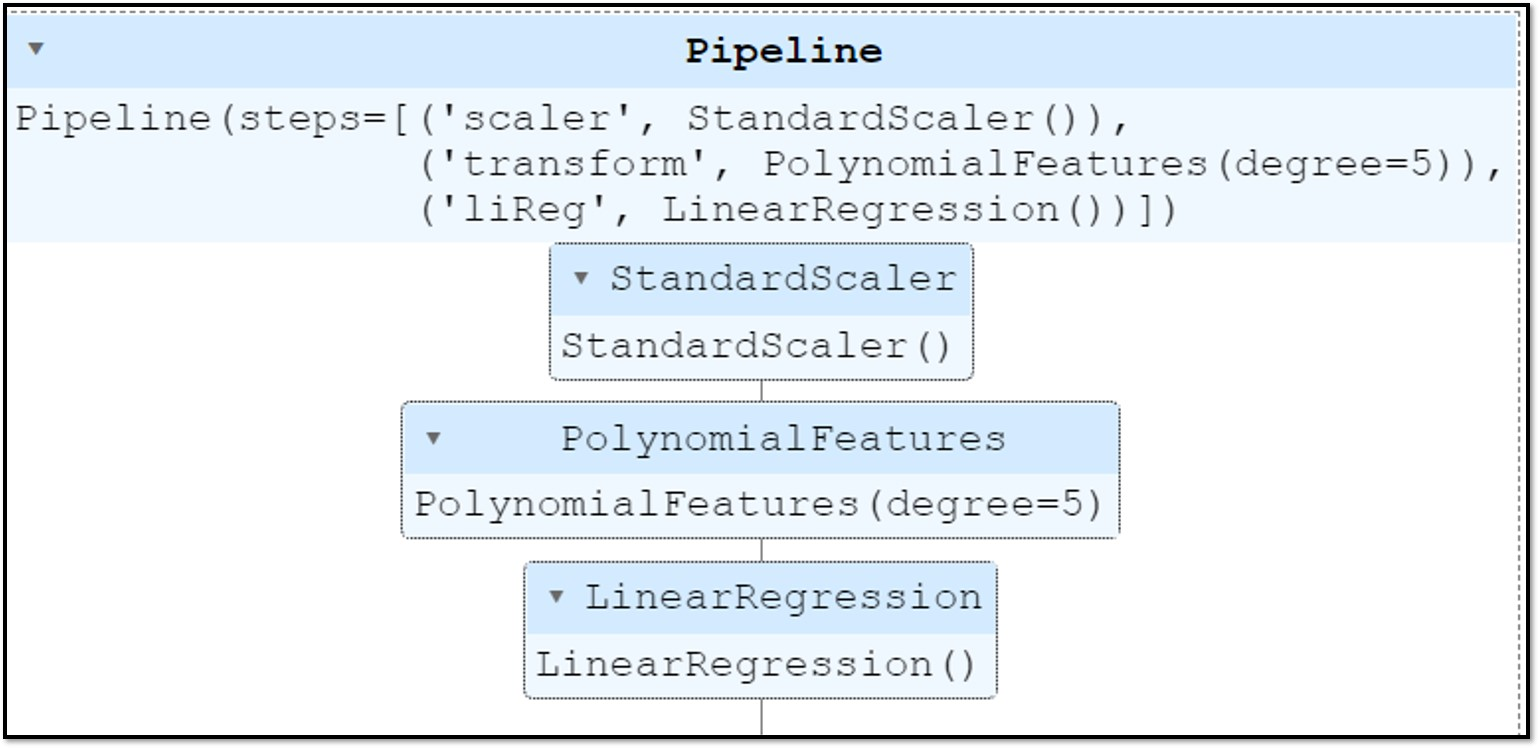
\includegraphics[width=8 cm]{pipeline.jpg}
  \caption{Pipeline for Modeling a Regression Model}
  \label{fig:pipeline}
\end{figure}

Figure \ref{fig:pipeline} summarizes the steps involved in implementing a regression model. The processes of feature scaling, polynomial transformation, and modeling can be done in one step by using the pipeline module in the sklearn library. This can make the process more efficient and organized, by chaining the different pre-processing and modeling steps together, and it can make it easy to try different combinations of pre-processing steps and models without having to repeat the same code over and over.

The following code demonstrates how to implement a polynomial regression model with a degree of 5 using the pipeline function. The pipeline function is used to combine the feature scaling using standardscaler function, polynomial transformation, and modeling steps into one step.

\begin{lstlisting}
# ==================================================#
from sklearn.pipeline import Pipeline

steps = [('scaler', StandardScaler()),
         ('poly', PolynomialFeatures(degree = 5)),
         ('liReg', LinearRegression())]

pipeline = Pipeline(steps)
pipeline.fit(X_train, y_train)
# ==================================================#
\end{lstlisting}

\newpage
\section{Performance Evaluation} \label{sec:evaluate}
This stage evaluates the predictive performance of the model using the test data set. There are different metrics to evaluate the model and the most common evaluation metrics are mean absolute error, mean squared error, and r2-score.

\subsection{Mean Absolute Error}

The mean absolute error (MAE) calculates how close the prediction is to the actual value on average and defines as:
\begin{equation}\label{mse}
  mae = \frac{1}{N} \sum_{i=1}^N |\tilde{y_i} - y_i|,
\end{equation}


\subsection{Mean Squared Error}
The mean squared error or root-mean squared error measures the average squared residuals (difference between the actual and the predicted values).
\begin{equation}\label{mse}
  mse = \frac{1}{N} \sum_{i=1}^N (\tilde{y_i} - y_i)^2,
\end{equation}

\begin{equation}\label{rmse}
  rmse = \sqrt{\frac{1}{N} \sum_{i=1}^N (\tilde{y_i} - y_i)^2},
\end{equation}

%MSE or RMSE is a good indicator to detect if the model predicted values that were significantly higher or lower than the actual values. If there is one or a few predicted values which are far away from the actual values, the mse or rmse will be significantly large compared to the mean absolute error.

\newpage
\subsection{R2-score}
R2 score, also known as the R-Squared score, is a metric that evaluates the goodness of fit of a regression model. It ranges from 0 to 1, with 1 indicating a perfect fit and 0 indicating a poor fit.
\begin{equation}\label{rmse}
  R^2 = 1- \frac{RSS}{TSS},
\end{equation} where $RSS$  is the sum of the squared differences between the predicted values and the actual values, while $TSS$ measures the total variance in the data by finding the sum of the squared differences between each data point and the average value. In other words, $TSS$ represents the total amount of variation in the data and $RSS$ represents the amount of variation that is not explained by the model. The definitions for $RSS$ and $TSS$ are as follows:

\begin{eqnarray}
% \nonumber to remove numbering (before each equation)$RSS$ 
  RSS &=& \sum_{i=1}^N (y_i-\tilde{y_i})^2 \\
  TSS &=& \sum_{i=1}^N (y_i-\bar{y_i})^2
\end{eqnarray} where $\tilde{y_i}$ is the predicted value and $\bar{y_i}$ is the mean value of the variable. 

The table below illustrates the calculation of $RSS$, $TSS$ and $R^2$ values in two extreme cases where $R^2=1$ and $R^2=0$.

\subsubsection{\textbf{Case 1: $R^2 = 1$}}
The first table demonstrates the first case when $R^2 = 1$. The predicted values are identical to the actual values, resulting in an $RSS$ value of zero. This scenario leads to an R2 score of 1, indicating a perfect fit of the data to the regression model. 

\begin{table}[h]
\centering
\begin{tabular}{|c|c|c|c| }
  \hline
  $y_i$ & $\tilde{y_i}$ & $(y_i-\tilde{y_i})^2$ & $(y_i-\bar{y_i})^2$  \\
  \hline
  10 & 10 & 0 & 100\\
  20 & 20 & 0 & 0\\
  30 & 30 & 0 & 100\\
  \hline
  $\bar{y_i}=20$ &  & RSS = 0  &  TSS = 200\\
  \hline
\end{tabular}
\caption{\textbf{Case 1}: Predicted and Actual Values are the same.}\label{tb:r2Case1}
\end{table}

\subsubsection{\textbf{Case 2: $R^2 = 0$}}
\begin{table}[h]
\centering
\begin{tabular}{|c|c|c|c| }
  \hline
  $y_i$ & $\tilde{y_i}$ & $(y_i-\tilde{y_i})^2$ & $(y_i-\bar{y_i})^2$  \\
  \hline
  10 & 20 & 100 & 100\\
  20 & 20 & 0 & 0\\
  30 & 20 & 100 & 100\\
  \hline
  $\bar{y_i}=20$ &  & RSS = 200  &  TSS = 200\\
  \hline
\end{tabular}
\caption{\textbf{Case 2}: Model always returns the average as predicted value.}\label{tb:r2Case2}
\end{table}

The second table illustrates the scenario where $R^2$  is 0, indicating a poor fit of the data to the regression model. In this case, the model always returns the average value of the actual data as the predicted value, resulting in an$RSS$ and $TSS$ value that are the same. This leads to an $R^2$ score of zero. 

It can be seen from these two examples that the R2 score ranges between 0 and 1, with a higher value indicating a better performance of the model. However, it's possible for the R2 score to be negative if the trained model performs worse than the baseline model which is returning the average values

It's worth mentioning that there is a variation of the R2 score called the adjusted R2 score, which takes into account the number of independent variables in the model. This metric helps in identifying irrelevant features in the model. However, the calculation of the adjusted R2 score is not covered in this book.

\newpage
\subsection{Implementation using Python}
The Python sklearn library offers a metrics module that can be used to compute various evaluation metrics for a model, such as R2 score. The functions in this module require the input of both the actual and predicted values. The predicted values can be obtained by using the 'predict' function of a trained model.

It is important to note that if any pre-processing steps were applied to the training data, such as feature scaling or polynomial transformation, the same pre-processing steps must be applied to the test data before using the model for evaluation. Failure to do so can result in a mismatch of feature spaces and negatively impact the model's performance.

However, it is crucial to ensure that the pre-processing parameters are only learned from the training data, and not from the test data. If information from the test data is used while building the model, it may appear to perform well on the test data but fail to perform well during actual deployment. This is known as "data leakage" problem, and it is crucial to avoid using any information from the test data while performing pre-processing steps to avoid such issues.

\subsubsection{\textbf{Evaluating the Linear Model}}
The code below demonstrates how to evaluate the multiple linear model that was previously trained. As the features were scaled using the standard scaler during training, it is necessary to scale the test data in the same way. The same mean and variance values used to transform the training data should be used to transform the test data, rather than learning new parameters from the test data set. 

In the sklearn library, this can be done by calling the 'transform' function during testing, as opposed to the 'fit\_transform' function used during training.

\begin{lstlisting}
# ==================================================#
from sklearn.metrics import mean_absolute_error
from sklearn.metrics import mean_squared_error
from sklearn.metrics import r2_score

X_test_scaled = scale.transform(X_test)
ytest_pred = lr.predict(X_test_scaled)

mae = mean_absolute_error(y_test, ytest_pred)
mse = mean_squared_error(y_test, ytest_pred,
                        squared= True)
r2 = r2_score(y_test, ytest_pred)
# ==================================================#
\end{lstlisting}
The root mean squared error (rmse) can be computed by setting the parameter \textbf{'squared'} to False.

\subsubsection{\textbf{Evaluating the Polynomial Model}}
When working with a polynomial regression model, it's important to remember that the same pre-processing steps used during training should be applied to the data before making predictions. In this case, the features were scaled using the standard scaler, and were also transformed using a fifth-order polynomial transform. Therefore, the same scaling and polynomial transformation steps should be applied to the data before making predictions with the model.

The code snippet below illustrates how to evaluate a polynomial regression model using a new test dataset in Python:

\begin{lstlisting}
# ==================================================#
from sklearn.metrics import mean_absolute_error
from sklearn.metrics import mean_squared_error
from sklearn.metrics import r2_score

X_test_scaled = scale.transform(X_test)
X_test_poly = poly.transform(X_test_scaled)
ytest_pred = lr_poly.predict(X_test_poly)

mae = mean_absolute_error(y_test, ytest_pred)
mse = mean_squared_error(y_test, ytest_pred,
                         squared= True)
r2 = r2_score(y_test, ytest_pred)
# ==================================================#
\end{lstlisting}


\subsubsection{\textbf{Evaluating the Pipeline}}

The sklearn library offers a "pipeline" function that can be used to prevent data leakage by ensuring that the appropriate pre-processing steps are applied to the correct data subset. With this function, it is not necessary to perform pre-processing steps separately, as the pipeline function takes care of it.

\begin{lstlisting}
# ==================================================#
from sklearn.metrics import mean_absolute_error
from sklearn.metrics import mean_squared_error
from sklearn.metrics import r2_score

ytest_pred = pipeline.predict(X_test)

mae = mean_absolute_error(y_test, ytest_pred)
mse = mean_squared_error(y_test, ytest_pred,
                        squared= True)
r2 = r2_score(y_test, ytest_pred)
# ==================================================#
\end{lstlisting}

\newpage
\subsection{Cross-Validation} \label{sec:cv}
Cross-validation is a technique that utilizes multiple test data sets to evaluate a model's performance, providing a more accurate idea of how the model will perform with new data. This is accomplished by first dividing the initial training data set into k subsets, known as folds. The model is then trained repetitively using k-1 subsets and tested on the remaining fold. This process is repeated until all folds have been used for testing. The model's performance is then evaluated for all folds and the average performance is reported.

The code below demonstrates how to use the Python sklearn "model\_selection" module to train a cross-validated polynomial regression model, making use of the pipeline function to avoid data leakage problems.

\begin{lstlisting}
# ==================================================#
from sklearn.model_selection import KFold
from sklearn.model_selection import cross_val_score

kfold = KFold(n_splits=5,shuffle=False)
steps = [('scaler', StandardScaler()),
         ('poly', PolynomialFeatures(degree = 4,
                                include_bias=False)),
         ('liReg', LinearRegression())]

pipeline = Pipeline(steps)
mse = -1*cross_val_score(pipeline, X_train, y_train,
                scoring = 'neg_mean_squared_error',
                cv=kfold)

print('average mean squared error is', np.mean(mse))
# ==================================================#
\end{lstlisting} The "KFold" function in the code snippet has a parameter named "n\_splits", which defines the number of subsets to be created, while the "cross\_val\_score" function provides a score (defined by the "scoring" parameter) for each fold. 

In this example, the number of splits is set to 5 and the scoring parameter is defined as negative mean squared error. This cross-validation method can also be used to optimize the hyper-parameters of a model using a grid search method, which will be covered in section \ref{sec:hyperP}.

\newpage
\subsection{Bias and Variance Trade-off}

The bias-variance trade-off is a fundamental concept in assessing the performance of supervised machine learning models.

\subsubsection{\textbf{Bias}}
Bias refers to the difference between a model's average prediction and the true value, and models that over-simplify and generalize relationships between variables fails to capture the actual trend in the data and tend to have a high bias. Simple linear regression models tend to have high bias and under-fit the data, resulting in large errors for both training and testing sets.

\subsubsection{\textbf{Variance}}
Variance measures how much the accuracy of a machine learning model can vary depending on the data set. It's common for a model to perform well on the training set but poorly on new or test data, which often occurs due to training on a small data set or over-fitting the training data, resulting in a loss of generalization.

\subsubsection{\textbf{Bias Variance Trade-off}}
\begin{figure}[!ht]
  \centering
  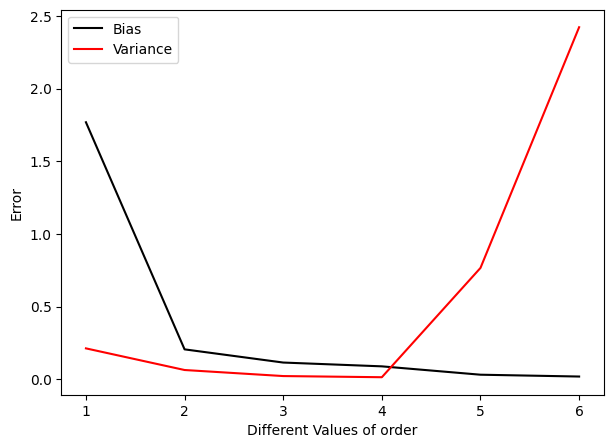
\includegraphics[width=8 cm]{Bias_Variance.png}
  \caption{Error vs. Order of regression model}
  \label{fig:bias_vari}
\end{figure}

Figure \ref{fig:bias_vari} illustrates how the model in the sales prediction example performs in relation to the order of the polynomial regression model. The error for the training data set (bias) decreases as the order of the polynomial regression model increases (i.e. the model becomes more complex), but the variance (difference in performance between training and testing data sets) increases with increasing model complexity.

A machine learning model should have an appropriate balance between bias and variance to avoid overfitting or underfitting the problem. In this example, the optimal result is achieved at order 4.


\newpage
\section{Regularization}\label{sec:regularization}

Regularization is a method to reduce over-fitting, particularly when there is a large variance between the train and test set performance. Regularization commonly achieved by modifying the loss function by adding a regularization term. This section will cover two popular regularization techniques: Lasso and Ridge Regression.

\subsection{Lasso Regression}
Lasso regression, also referred to as L1 regularization, is a technique that adds a penalty term based on the absolute value of the coefficient magnitude to the loss function.

\begin{equation}\label{eq:Lassocost}
  \varepsilon = \frac{1}{N}\sum_{i=1}^N (\tilde{y_i}-y_i)^2 + \alpha \sum_{j = 1}^{N_p} \parallel \omega_j \parallel,
\end{equation} where $N$ is the number of data points and $\tilde{y_i}$ is the predicted value using the model, $N_p$ is the number of parameters, $\omega_j, j = 1, 2, ..., N_p$ are parameters of the model and the parameter $\alpha$ controls the amount of regularization.

The parameter $\alpha$ reduces the value of coefficients and when it's sufficiently large, some of the coefficients $\omega_i$ will be eliminated. Therefore, Lasso regression is particularly useful when the model is suffering from multi-collinearity or when working with high dimensional data (number of features is more than the number of observations) and wanting to remove some of the less important features automatically.


\subsection{Ridge Regression}
Ridge regression is similar to Lasso regression, but instead of adding an $L1$ penalty term it adds an $L2$ norm penalty term to the loss function.

\begin{equation}\label{eq:ridgecost}
  \varepsilon = \frac{1}{N}\sum_{i=1}^N (\tilde{y_i}-y_i)^2 + \alpha \sum_{j = 1}^{N_p} \omega_j ^2,
\end{equation} where $N$ is the number of data points and $\tilde{y_i}$ is the predicted value using the model, $N_p$ is the number of parameters, $\omega_j, j = 1, 2, ..., N_p$ are parameters of the model and the parameter $\alpha$ controls the amount of regularization.

Unlike Lasso, Ridge regression never eliminates coefficients and thus, can't be used for automatic feature selection.

\newpage
\subsection{Lasso vs. Ridge}
In the example of predicting sales amount, three advertisement programs were used to predict the sale amount and the multiple linear regression model is represented as:

\begin{equation}\label{eq:polyResult}
  y = 3.893 x_1 + 3.420 x_2 + 2.943 x_3 + 13.788,
\end{equation} where $x_i$ are independent features. It can be observed that the variable $x_1$ is the most significant feature and has the highest coefficient.

\begin{table}[!ht]
\centering
\begin{tabular}{|c|r|r|r|r|}
  \hline
               & $\alpha = 0$  & $\alpha = 0.5$ & $\alpha = 1$ & $\alpha = 10$ \\
  \hline
  $\omega_1$ (L) & 3.893 & 3.420 & 2.943 & 0 \\
  $\omega_2$ (L) & 2.761 & 2.310 & 1.832 & 0 \\
  $\omega_3$ (L) & 0.067 & 0 & 0 & 0 \\
  \hline
  \hline
  $\omega_1$ (R) & 3.893 & 3.879 & 3.865 & 3.625 \\
  $\omega_2$ (R) & 2.761 & 2.749 & 2.738 & 2.546 \\
  $\omega_3$ (R) & 0.067 & 0.072 & 0.078 & 0.163 \\
  \hline
  \hline
\end{tabular}
\caption{Effects of the regularized parameter $\alpha$  on the Parameters}\label{tb:regular}
\end{table}

In this section, the model from the previous example of sales amount prediction is re-implemented using Ridge and Lasso regression with various regularization weights.

Table \ref{tb:regular} illustrates the effect of the regularization parameter $\alpha$ on the magnitude of coefficients in the Lasso and Ridge models. It is important to note that this implementation is only done to demonstrate the effect of the regularization parameter and regularization is not needed for this problem.

As we can see, Lasso regression eliminates coefficients for the least important variable $x_3$ when the parameter $\alpha$ becomes sufficiently large ($\alpha \geq 10$), while Ridge regression reduces the magnitude of high coefficients but keeps lower coefficient values.

\newpage
\section{Hyper-Parameter Tuning}\label{sec:hyperP}
Hyper-parameters are parameters that are set before modeling begins. Examples of typical parameters for a regression model include the order of a polynomial regression model, $k$, and the regularization parameter $\alpha$ in Lasso and Ridge models. The cross-validation method discussed in section \ref{sec:cv} is often used to find the best hyper-parameters for a machine learning model. These parameters are then used to develop a model that is deployed and tested on an initial testing data-set.

Grid search and random search are common methods for finding the best hyper-parameters for a model. These methods define a parameter space that includes a set of possible hyper-parameter values that can be used to build the model. Grid search method uses every combination of hyper-parameter values to train the model and select the best hyper-parameter. Random search method randomly selects and tests a random combination of hyper-parameters and it is more efficient than grid search for a higher number of parameters. 

The code below shows an example of how to find the hyper-parameter $k$ for a polynomial regression model using the Grid search method.


\newpage

\begin{lstlisting}
# ==================================================#
from sklearn.model_selection import GridSearchCV

steps = [('scaler', StandardScaler()),
         ('poly', PolynomialFeatures(degree = order,
                                include_bias=False)),
         ('liReg', LinearRegression())]
parameters = {"poly__degree":[1, 4, 6, 9]}
pipeline = Pipeline(steps)

poly_grid = GridSearchCV(pipeline, parameters,
                         cv=4,
                        scoring='neg_mean_squared_error')

poly_grid.fit(X_train, y_train)
print ('best order is :', poly_grid.best_params_)

y_pred_test = poly_grid.predict(X_test)
mae = mean_absolute_error(y_test, y_pred_test)
# ==================================================#
\end{lstlisting}



\newpage
\section{Project: Sale Amount Prediction}\label{sec:LRproject1}

A complete example for predicting the sale amount based on different advertisement programs is provided below. The data set used in this example is small, containing four features and 200 rows of entries. The "sale amount" is the target feature, and the other three features are the costs associated with the "TV", "radio", and "newspaper" programs. The data set can be downloaded from the provided \href{https://www.kaggle.com/sazid28/advertising.csv}{link}\cite{web:adData}. Note that the data has already been cleaned and no missing data is present.

\subsection{Data Importing}
The initial step is to import the required modules and then read the data from the computer.

\begin{lstlisting}
# ==================================================#
import pandas as pd

df=pd.read_csv('..\\data\Advertising.csv')

X=df[['TV', 'radio', 'newspaper']].values
y=df['sales'].values

# ==================================================#
\end{lstlisting}

\newpage
\subsection{Train-Test-Split}
The data is divided into training and testing data sets. Two-thirds of the data is allocated for training, and the remaining one-third is reserved for testing.
\begin{lstlisting}
# ==================================================#
from sklearn.model_selection import train_test_split

X_train, X_test, y_train, y_test = train_test_split(X,y,
                                    test_size = 0.33,
                                    random_state=1)
# ==================================================#
\end{lstlisting}

\newpage
\subsection{Modeling and Hyper-Parameter Tuning}
The grid search method is applied to determine the hyper-parameter $k$, which is the order of the polynomial regression model. The pipeline function is utilized to prevent potential data leakage issues.

\begin{lstlisting}
# ==================================================#
from sklearn.model_selection import GridSearchCV
from sklearn.preprocessing import StandardScaler
from sklearn.preprocessing import PolynomialFeatures
from sklearn.linear_model import LinearRegression
from sklearn.pipeline import Pipeline

steps = [('scaler', StandardScaler()),
         ('poly', PolynomialFeatures(degree = 2,
                                include_bias=False)),
         ('liReg', LinearRegression())]
parameters = {"poly__degree":[2, 3, 4, 5, 7, 9]}
pipeline = Pipeline(steps)
poly_grid = GridSearchCV(pipeline, parameters,
                         cv=5,
                        scoring='neg_mean_squared_error',
                        verbose= True)
poly_grid.fit(X_train, y_train)
print ('best order is :', poly_grid.best_params_)
# ==================================================#
\end{lstlisting}

\newpage
\subsection{Model Evaluation}
The performance of the best model is evaluated on both the training and testing data sets.

\begin{lstlisting}
# ==================================================#
rom sklearn.metrics import mean_absolute_error
from sklearn.metrics import mean_squared_error
from sklearn.metrics import r2_score

# Evaluation on the Tesing data set
ytest_pred = poly_grid.predict(X_test)
mae = mean_absolute_error(y_test, ytest_pred)
mse = mean_squared_error(y_test, ytest_pred,
                        squared= True)
r2 = r2_score(y_test, ytest_pred)
#Evaluation on the Training data set
ytr_pred = poly_grid.predict(X_train)
maeT = mean_absolute_error(y_train, ytr_pred)
mseT = mean_squared_error(y_train, ytr_pred,
                        squared= True)
r2T = r2_score(y_train, ytr_pred)
#Keep all results in the tabular form
result = pd.DataFrame({'mae': [maeT, mae],
                        'mse': [mseT, mse],
                        'r2': [r2T, r2]})
result.index = ['Training', 'Testing']
# ==================================================#
\end{lstlisting}

It is suggested that readers download the full codes and data sets from the public \href{https://github.com/myothida/Intro-To-Supervised-Machine-Learning.git}{\textbf{GitHub Repo}} and experiment with running the code using different data sets.

%----------------------------------------------------------------------------------------
%	CHAPTER THREE
%----------------------------------------------------------------------------------------

\chapter{Classification}

\epigraph{Classification is the act or process of dividing things into groups according to their type. }{\textit{Cambridge dictionary}}

Classification in machine learning involves assigning input data to a specific class label based on information learned from training data. An example of this is a bio-authentication system where a face is classified as either "authorized" or "rejected" based on pre-trained information. The concepts from regression methods, such as training and testing data sets, residuals or errors, cost function, and independent variables, also apply to classification.

In the project discussed in section \ref{sec:LRproject1}, the sale amount is predicted based on the advertising cost. As an illustration, consider a scenario where we want to determine whether a predicted sales amount meets a target or not. The output can only be two values: "meets the target" (yes) or "does not meet the target" (no). This is known as a \emph{binary classification} problem, as there are only two possible outputs: "yes" and "no".


Binary classification problems are commonly used in identifying specific outcomes based on the labelled data, such as:
\begin{itemize}
  \item Determining whether an email is spam (1) or not (0)
  \item Identifying if a tumor is malignant (1) or benign (0)
  \item Predicting if a customer will default on a loan (1) or not (0) based on their behavior.
\end{itemize}


A \textbf{multi-class classification} problem involves assigning an input to one of more than two possible classes. For example, consider a task of labeling names from 135 different races in Myanmar, where the goal is to classify each name into one of the 135 races.

Another type of classification problem is called \textbf{multi-label classification}, where an input can be assigned to multiple classes. This type of problem is commonly found in text categorization, where a text document may belong to multiple labels or categories.

\newpage
\section{Performance Evaluation}\label{sec:Clsevaluation}

This section discusses the most commonly used metrics for evaluating the performance of a classification model, specifically in the context of binary classification problems. These metrics include measures such as accuracy, precision, recall, F1 score, and ROC-AUC. It is important to note that there is no one-size-fit-all metric to measure the performance of a classification model.

Each of these metrics has its own unique characteristics and is better suited for certain types of classification problems. For example, accuracy is a good metric when the classes are balanced, but precision and recall are more appropriate when the classes are imbalanced. Additionally, the ROC-AUC metric is widely used for evaluating the performance of models that predict probabilities. The appropriate metric to be used will depend on the specific problem at hand and context.

The metrics used to evaluate performance in binary classification problems can be applied to multi-class classification problems by calculating them for each class and then taking the average.

\subsection{Confusion Matrix}
In binary classification problem, there are only two possible outputs: one and zero.
\begin{table}[!ht]
\centering
\begin{tabular}{|c|c|c|c|c|c|c| }
    \hline
    Predicted output & 0 & 1 & 0 & 0 & 1 & 1  \\
    \hline
    Actual Label & 0 & 0 & 1 & 0 & 0 & 1\\
    \hline
\end{tabular}
\caption{Example labels of predicted and actual output.}\label{tb:cmTable}
\end{table}

Table \ref{tb:cmTable} illustrates examples of predicted outputs and actual labels, with four possible combinations:
\begin{itemize}
  \item Case 1: Predicted as one and actual value is one (11)
  \item Case 2: Predicted as one but actual value is zero (10)
  \item Case 3: Predicted as zero and actual value is one  (01)
  \item Case 4: Predicted as zero and actual value is zero (00)
\end{itemize}

A successful classification model will have a higher ratio of cases 1 and 4 and a lower ratio of cases 2 and 3. Table \ref{tb:cmTable} illustrates that there are 1 number of case 1 (11), 2 number of case 2 (10), 1 number of case 3 (01) and 2 number of case 4 (00). This information can be summarized in a square matrix form below:

\begin{figure}[!h]
  \centering
  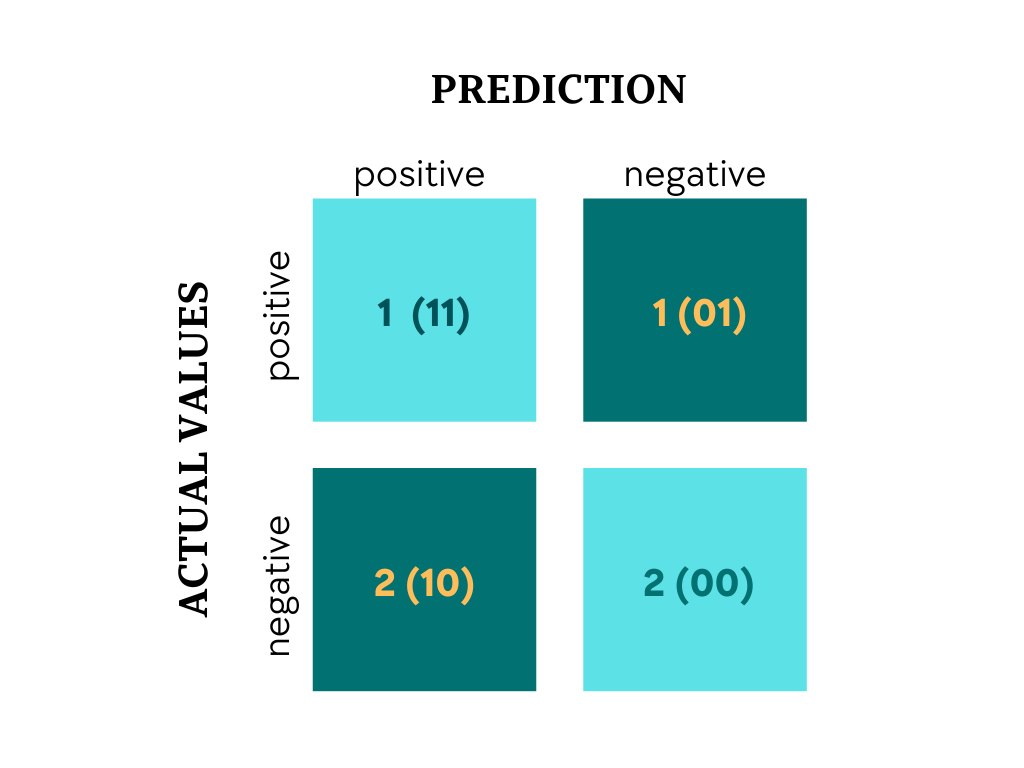
\includegraphics[width=9 cm]{CM_eg.png}
  \caption{Confusion Matrix for Table \ref{tb:cmTable}}
  \label{fig:cm_eg}
\end{figure}

The first column represents the instances where the model predicted a positive outcome. Out of the 3 instances where the model predicted positive, one was correct as the actual value was also positive. This is reflected in the top-left box. The remaining 2 instances were incorrect predictions, as the actual value was negative, and this is reflected in the bottom-left box.

The second column represents the instances where the model predicted a negative outcome. Out of the 3 instances where the model predicted negative, two were correct as the actual values were also negative. This is reflected in the bottom-right box. The remaining one was an incorrect prediction, as the actual value was positive, and this is reflected in the top-right box.

\begin{figure}[!h]
  \centering
  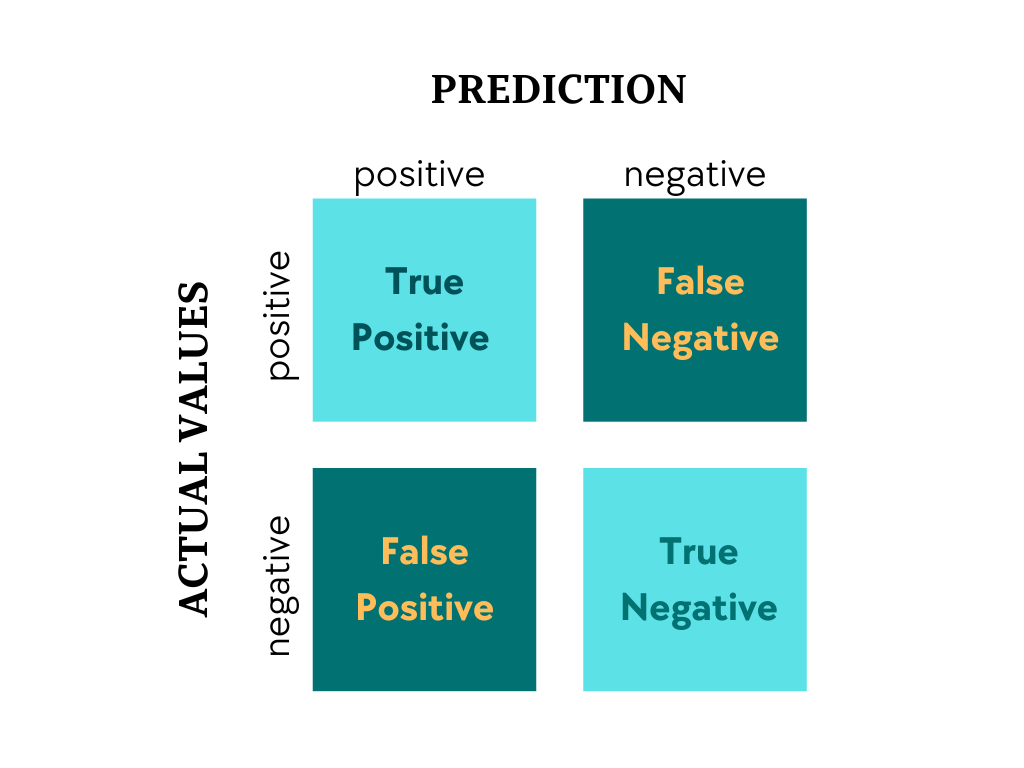
\includegraphics[width=8 cm]{Classifier_CM.png}
  \caption{Confusion Matrix: rows (Actual) and columns (Prediction)}
  \label{fig:cls_cm}
\end{figure}

In general, a \textbf{confusion matrix} is a table that summarizes the performance of a classification model by comparing predicted values with actual values. (Refer to Figure \ref{fig:cls_cm}.) It typically has four quadrants, each representing one of the following outcomes:

\begin{itemize}
  \item True Positive (\textbf{TP}) refers to instances where the model predicted a positive outcome and the actual value was also positive.
  \item False Positive (\textbf{FP}) refers to instances where the model predicted a positive outcome but the actual value was negative.
  \item False Negative (\textbf{FN}) refers to instances where the model predicted a negative outcome but the actual value was positive.
  \item True Negative (\textbf{TN}) refers to instances where the model predicted a negative outcome and the actual value was also negative.
\end{itemize}

In this book, we align with the convention used in the Python sklearn library where the rows of the confusion matrix represent the actual values and the columns represent the predicted values. However, it is worth noting that there is another common format of the confusion matrix where the rows represent the predicted values and the columns represent the actual values.

\subsection{Accuracy}
Accuracy is a metric that quantifies the proportion of correct predictions made by a model. Using the example in Table 3.1, there are six predictions made and three of them are correct, the accuracy of the model is 50\%. Mathematically, the formula for calculating accuracy is defined as:

\begin{equation}\label{eqn_acc}
  Accuracy = \frac{TP + TN}{TP+FP+FN+TN}
\end{equation}

However, accuracy is not always an appropriate metric to evaluate the performance of a model when the classes are imbalanced. For example, let's consider a scenario where there are 15 positive cases and 85 negative cases.
\begin{figure}[!h]
  \centering
    \begin{subfigure}[b]{0.7\textwidth}
         \centering
         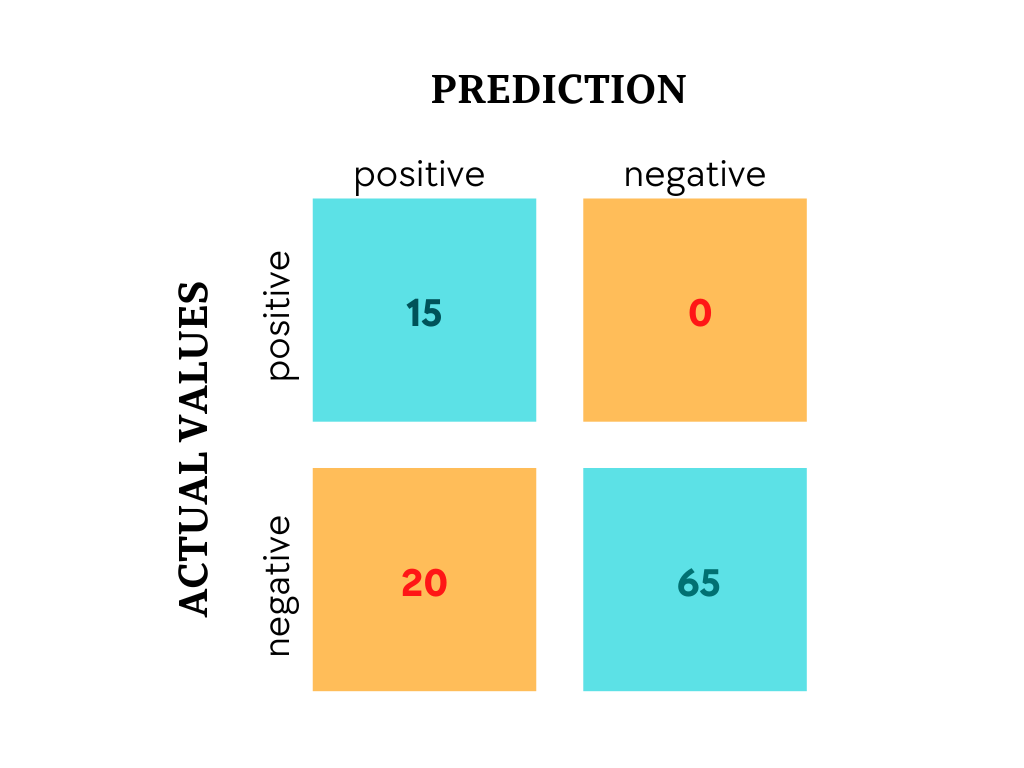
\includegraphics[width=5 cm]{cm_3e.png}
         \caption{Model 1}
         \label{fig:mdoel1_cm}
     \end{subfigure}
     \begin{subfigure}[b]{0.7\textwidth}
         \centering
         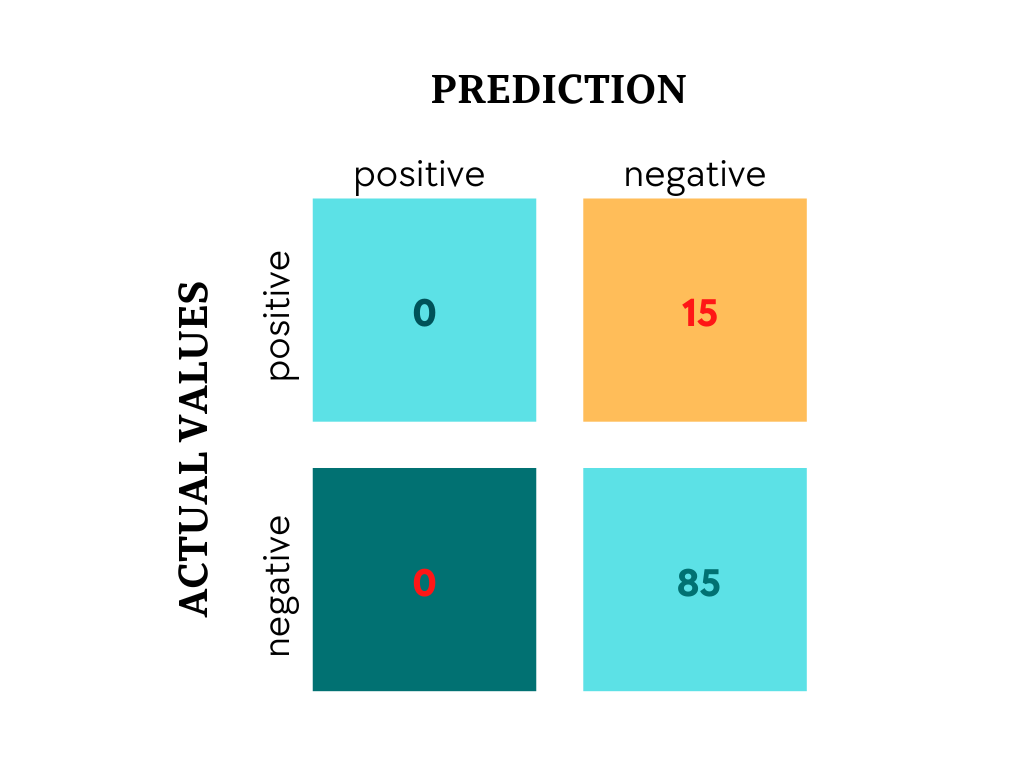
\includegraphics[width=5 cm]{cm_4e.png}
         \caption{Model 2}
         \label{fig:mdoel2_cm}
     \end{subfigure}
  \caption{Confusion Matrix from Model 1 and Model 2}
  \label{fig:cls_cm_Imb}
\end{figure} The confusion matrices for Model 1 and Model 2 are shown in Figure \ref{fig:cls_cm_Imb}. From the confusion matrices, it can be seen that Model 1 (Refer to Figure \ref{fig:mdoel1_cm}) has only $80\%$ accuracy and Model 2 (Refer to Figure \ref{fig:mdoel1_cm}) has $85\%$ accuracy. However, if we examine the confusion matrices carefully, Model 1 accurately predicts all positive cases and $76\%$ of the negative cases (75 out of 85), while Model 2 (Refer to Figure \ref{fig:mdoel2_cm}) did not detect any of the positive cases. If these models are developed for cancer detection, Model 2 is missing all the cancer patients.

In such scenarios, other metrics such as precision and recall should be considered.

\subsection{Precision}
Precision measures the proportion of true positive predictions out of all positive predictions made by a model and it is calculated as:
\begin{equation}\label{eqn_prec}
  Precision = \frac{TP}{TP+FP}
\end{equation}Precision is particularly important when minimizing false positives is a higher priority than minimizing false negatives. For example, in the case of a spam filter, it is more important to avoid marking a legitimate email as spam (false positive) than to allow a spam email to reach the inbox (false negative). High precision is therefore critical in problem like spam filtering systems.

\subsection{Recall (Sensitivity)}
Recall, also know as sensitivity or true positive rate, measures the proportion of actual positive cases that were correctly identified by the model and it is calculated as:
\begin{equation}\label{eqn_recall}
  Recall (\text{sensitivity}) = \frac{TP}{TP+FN}
\end{equation}Recall is particularly important in cases where missing a positive case (false negative) is more detrimental than having false alarms (false positives). This is often the case in medical applications such as cancer detection, where missing a cancer case is more dangerous than detecting one in a non-cancer patient. In such scenarios, recall should be as high as possible.

%Recall is also known as sensitivity, as it measures how well a model can detect positive cases and true positive rate, as it is calculated by dividing the number of accurately detected positive cases by the total number of actual positive cases.
%\newpage
\subsection{True Negative Rate (Specificity)}
The specificity, also known as the true negative rate, measures how many negative cases are accurately detected by the model. It is calculated as::
\begin{equation}\label{eqn_specificity}
  TNR (\text{Specificity}) = \frac{TN}{FP+TN}
\end{equation} Specificity is particularly useful when the cost of a false positive (predicting a negative case as positive) is high. An example of this can be a medical test for a rare disease. In this case, a false positive would mean that a healthy person is incorrectly diagnosed as having the disease, which would have severe consequences. In such scenarios, a high specificity is desired.

\subsection{F-score}
F-score, also known as F1-score, is a metric that combines both precision and recall into a single score, it is defined as:
\begin{equation}\label{eqn_Fscore}
  F-score = \frac{2*Recall*Precision}{Recall+Precision}
\end{equation}The F-score is high when both precision and recall are high, and low when either one of them has a low value. It is particularly effective in problems where both false positives and false negatives are considered equally important.
\newpage
\subsection{Area under the ROC (AUROC or AUC)}
The area under the ROC (receiver operating characteristic) curve is a widely used evaluation metric that measures a model's ability to distinguish between classes. It is calculated as the area under the Receiver Operating Characteristic (ROC) curve and AUC ranges between 0 and 1, with a value of 1 indicating a perfect classifier and a value of 0.5 indicating a classifier that is no better than random guessing.

AUC is commonly used to evaluate the performance of a model when the proportion of positive and negative cases is imbalanced. A high AUC value indicates that the model is able to correctly classify a large proportion of positive cases while also correctly classifying a large proportion of negative cases.

\noindent To understand AUC, it is important to first understand the ROC curve which plots two metrics:
\begin{itemize}
  \item True Positive Rate (TPR, also known as recall)
  \item False Positive Rate (FPR, which is 1 - specificity)
\end{itemize}

Many classification methods, such as logistic regression, produce a probability of an input belonging to the positive class. The class label is then obtained by comparing the resulting probability with a pre-defined threshold. A higher threshold value will reduce the number of positive predictions (both TP and FP).

\begin{table}[!h]
\centering
\begin{tabular}{|c|c|c|c|c|}
  \hline
  Threshold & TP & TN & TPR & FPR \\
  \hline
  0   & 117 & 0 & 1 & 1 \\
  \hline
  0.2 & 101 & 7013 & 0.863 & 0.001 \\
  \hline
  0.5(default) & 93 & 7037 & 0.795 & 0.0007 \\
  \hline
  0.8 & 93 & 7039 & 0.752 & 0.0004 \\
  \hline
  1 & 0 & 7042 & 0 & 0 \\
  \hline
\end{tabular}
\caption{Trade-off between TPR and FPR.}\label{tb:roc}
\end{table}

\begin{figure}[!h]
  \centering
  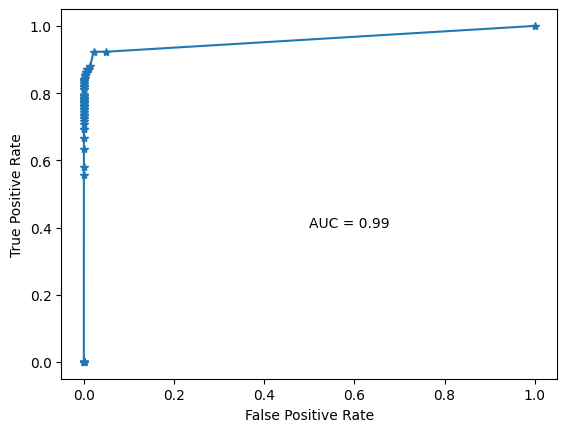
\includegraphics[width=7.5 cm]{auc.png}
  \caption{Binary ROC curve}
  \label{fig:auc}
\end{figure}

This is demonstrated in Table \ref{tb:roc}. There are $117$ actual positive cases (FN + TP) and $7042$ negative cases (TN + FP). When the threshold value is set to zero, all predictions are classified as positive cases, resulting in all positive cases correctly classified (TP = 117), and the true positive rate TPR is 1. As the threshold value increases, the true positive will decrease but the true negative will increase.

At the other extreme case, when the threshold value is set to 1, all cases are predicted as negative class, resulting in all negative cases correctly classified (TN = 7042) but none of the positive classes will be detected.

The ROC curve plots the true positive rate against the false positive rate, as shown in Figure \ref{fig:auc}. The AUC is computed by measuring the area under this curve. In this example, the model has a high AUC score of 0.99, indicating that it has a strong ability to accurately identify both positive and negative cases.


\newpage

\section{Logistic Regression}

Logistic regression maps input values to estimated target classes. It uses a sigmoid function, also known as the logistic function, to make predictions. Mathematically, it is defined as:
\begin{equation}\label{eq:ypredLR}
   \tilde{y} = g(\theta^T x) = \frac{1}{1+\exp(-\theta^T x)},
\end{equation}where $\theta$ is the model parameters and $x$ denotes an independent variable. In the case of a single feature, $\theta^T x$ is equal to $\omega_1 x + b$. The predicted values of $\tilde{y}$ can be interpreted as the probability of the target belong to the class 1 (or positive case) and it will always be between $0$ and $1$. This can be further illustrated by plotting the $g(z)$:

\begin{equation}\label{eq:ypredLR_z}
   g(z) = \frac{1}{1+\exp(-z)},
\end{equation} where $z$ is defined as $z = \theta^T x$.

Figure \ref{fig:sigmoid} illustrates that the output of the sigmoid function (g(z)) is always limited between 0 and 1. When the input value ($z$) approaches infinity, the output ($g(z)$) approaches 0 and when the input value ($z$) approaches negative infinity, the output ($g(z)$) approaches 1.  The predicted outputs (class labels) are obtained by applying a threshold value to the output of the sigmoid function $\tilde{y}$. The threshold value is usually set at 0.5 to classify the class label as either 0 or 1.

\begin{figure}[!h]
  \centering
  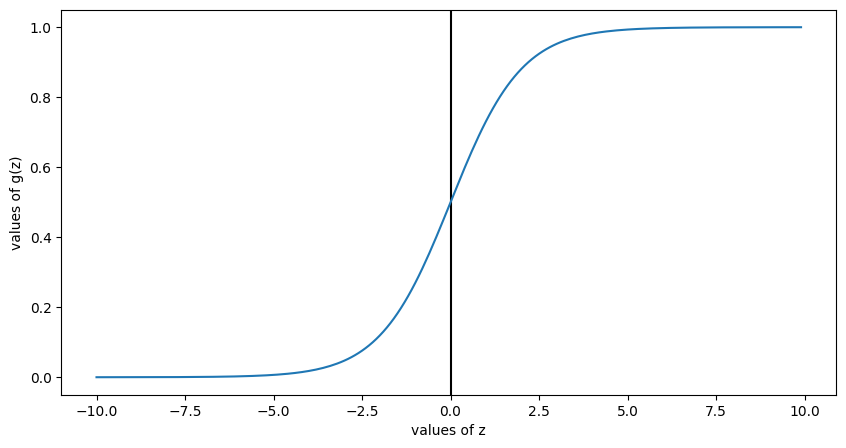
\includegraphics[width=8 cm]{demo_LR.png}
  \caption{Demonstration of Sigmoid Function}
  \label{fig:sigmoid}
\end{figure}

Since the target variable ($y$) in a binary classification problem is a categorical value that can only be 0 or 1, the cost function in logistic regression utilizes this property to predict the target class and the cost is defined as:
\begin{equation}\label{eqn:cost_LogR}
  J(\theta) = cost(g(z), y_i) = \begin{cases}
                    -\log (g(z)) &     \text{if $y_i = 1$}\\
                                 & \\
                    -\log (1-g(z)) &  \text{if $y_i = 0$}
                    \end{cases}
\end{equation} The above equation can be combined into a single equation as:
\begin{equation}\label{eqn:cost_LogR2}
  J(\theta) = -y_i \log (g(z)) - (1-y_i) * \log (1-g(z))
\end{equation}


If the estimated label $g(z)$ is the same with the actual output $y$, the cost value will be zero as shown in Table \ref{tb:LRcostR}.
\begin{table}[!ht]
\centering
\begin{tabular}{|c|c|r|}
  \hline
  Actual  & Estimated label & cost \\
  \hline
  & & $J(\theta) = -\log (g(z))$\\
  \hline
  $y =1$ & $g(z)=1$ & $J(\theta) = -\log (1)=0$\\
  $y =1$ & $g(z)=0$ & $J(\theta) = -\log (0)=1$\\
  \hline
  & & $J(\theta) = -\log (1-g(z))$\\
  \hline
  $y =0$ & $g(z)=1$ & $J(\theta) = -\log (1-1)=-1$\\
  $y =0$ & $g(z)=0$ & $J(\theta) = -\log (1-0)=0$\\
  \hline
\end{tabular}
\caption{Results of Cost function in \ref{eqn:cost_LogR}.}\label{tb:LRcostR}
\end{table}


In general, for multiple number of observations, the cost function can be defined as an average of the cost values for all observations.
\begin{equation}\label{eqn:cost_LogR_F}
  J(\theta) = -\frac{1}{N} \sum_{i=1}^N \left[y_i*log (g(z) + (1-y_i)*log(1-g(z)\right]
\end{equation} where $N$ is the number of data points (sample or observations). We can use an optimization algorithm, such as the gradient descent method discussed in section \ref{sec:GDS}, to find the best parameter $\theta$ that minimizes the cost.


\newpage

\subsection{Logistic Regression in Python}

The following code demonstrates the implementation of a logistic regression classifier using Python's sklearn library. The same steps outlined in section \ref{sec:model} are also applied in this example.

The 'fraud' data set \cite{web:fraudData} is used to predict whether a borrower will default or not, where default is defined as the borrower failing to make required payments on a debt. There are 30 features in the data set, with the target variable (default or non-default) listed in the 'Class' column. The remaining 29 columns are used as independent features.

\begin{lstlisting}[language=Python]
# ==================================================#
import pandas as pd

df=pd.read_csv('..\\data\\fraud.csv')
y = df['Class'].values
X = df.drop(columns = 'Class').values

from sklearn.model_selection import train_test_split

X_train, X_test, y_train, y_test = train_test_split(X,y,
                                    test_size = 0.33,
                                    random_state=1)

#--------------------------------------------------
## Using piepline to implement Logistic regression ##
#--------------------------------------------------
from sklearn.preprocessing import StandardScaler
from sklearn.linear_model import LogisticRegression
from sklearn.pipeline import Pipeline

steps = [('scaler', StandardScaler()),
         ('logReg', LogisticRegression())]

clf_pipeline = Pipeline(steps)
clf_pipeline.fit(X_train, y_train)
#--------------------------------------------------
## Model Evaluation ##
#--------------------------------------------------
from sklearn.metrics import classification_report
from sklearn.metrics import confusion_matrix
from sklearn.metrics import roc_auc_score

ypred_test = clf_pipeline.predict(X_test)
mat_clf = confusion_matrix(y_test, ypred_test)
report_clf = classification_report(y_test, ypred_test)

ypred_testP = clf_pipeline.predict_proba(X_test)
auc = roc_auc_score(y_test, ypred_testP[:,1])
# ==================================================#
\end{lstlisting}

\subsection{Hyper-parameters}
There are several optimization algorithms that can be used to solve the optimization problem in logistic regression, such as Newton method and Stochastic Average Gradient (SAG). The choice of solver is a hyperparameter in implementing the logistic regression method and can be determined through methods such as grid or random search. However, in-depth explanation of different optimization algorithms is outside the scope of this book.

Another important hyperparameter for logistic regression is the strength of the regularization term, which can help to prevent over-fitting as discussed in section \ref{sec:regularization}. The Python sklearn library offers various options for setting hyper-parameters in the Logistic Regression function, and more information can be found in the \href{https://scikit-learn.org/stable/modules/linear_model.html#logistic-regression}{sickit documentation} \cite{web:sklearn}.




\newpage

\section{K Nearest Neighbors or k-NN}

\epigraph{Birds of a feather flock together. }{\textit{Proverb}}

The K nearest neighbor (k-NN) classification method is one of the simplest and easiest to understand. Imagine you are a new student in my class and I do not know much about you yet, but I see that you hang out with good students. Intuitively, I would assume that you would also be a good student. The same concept is used in k-NN, where:
\begin{itemize}
  \item the distance from a new data point to the other data points in the training data-set is calculated
  \item the K neighbors closest to the new data point are selected
  \item the new data point is assigned to the group of the majority of the nearest K data points.
\end{itemize}

\begin{figure}[!h]
  \centering
  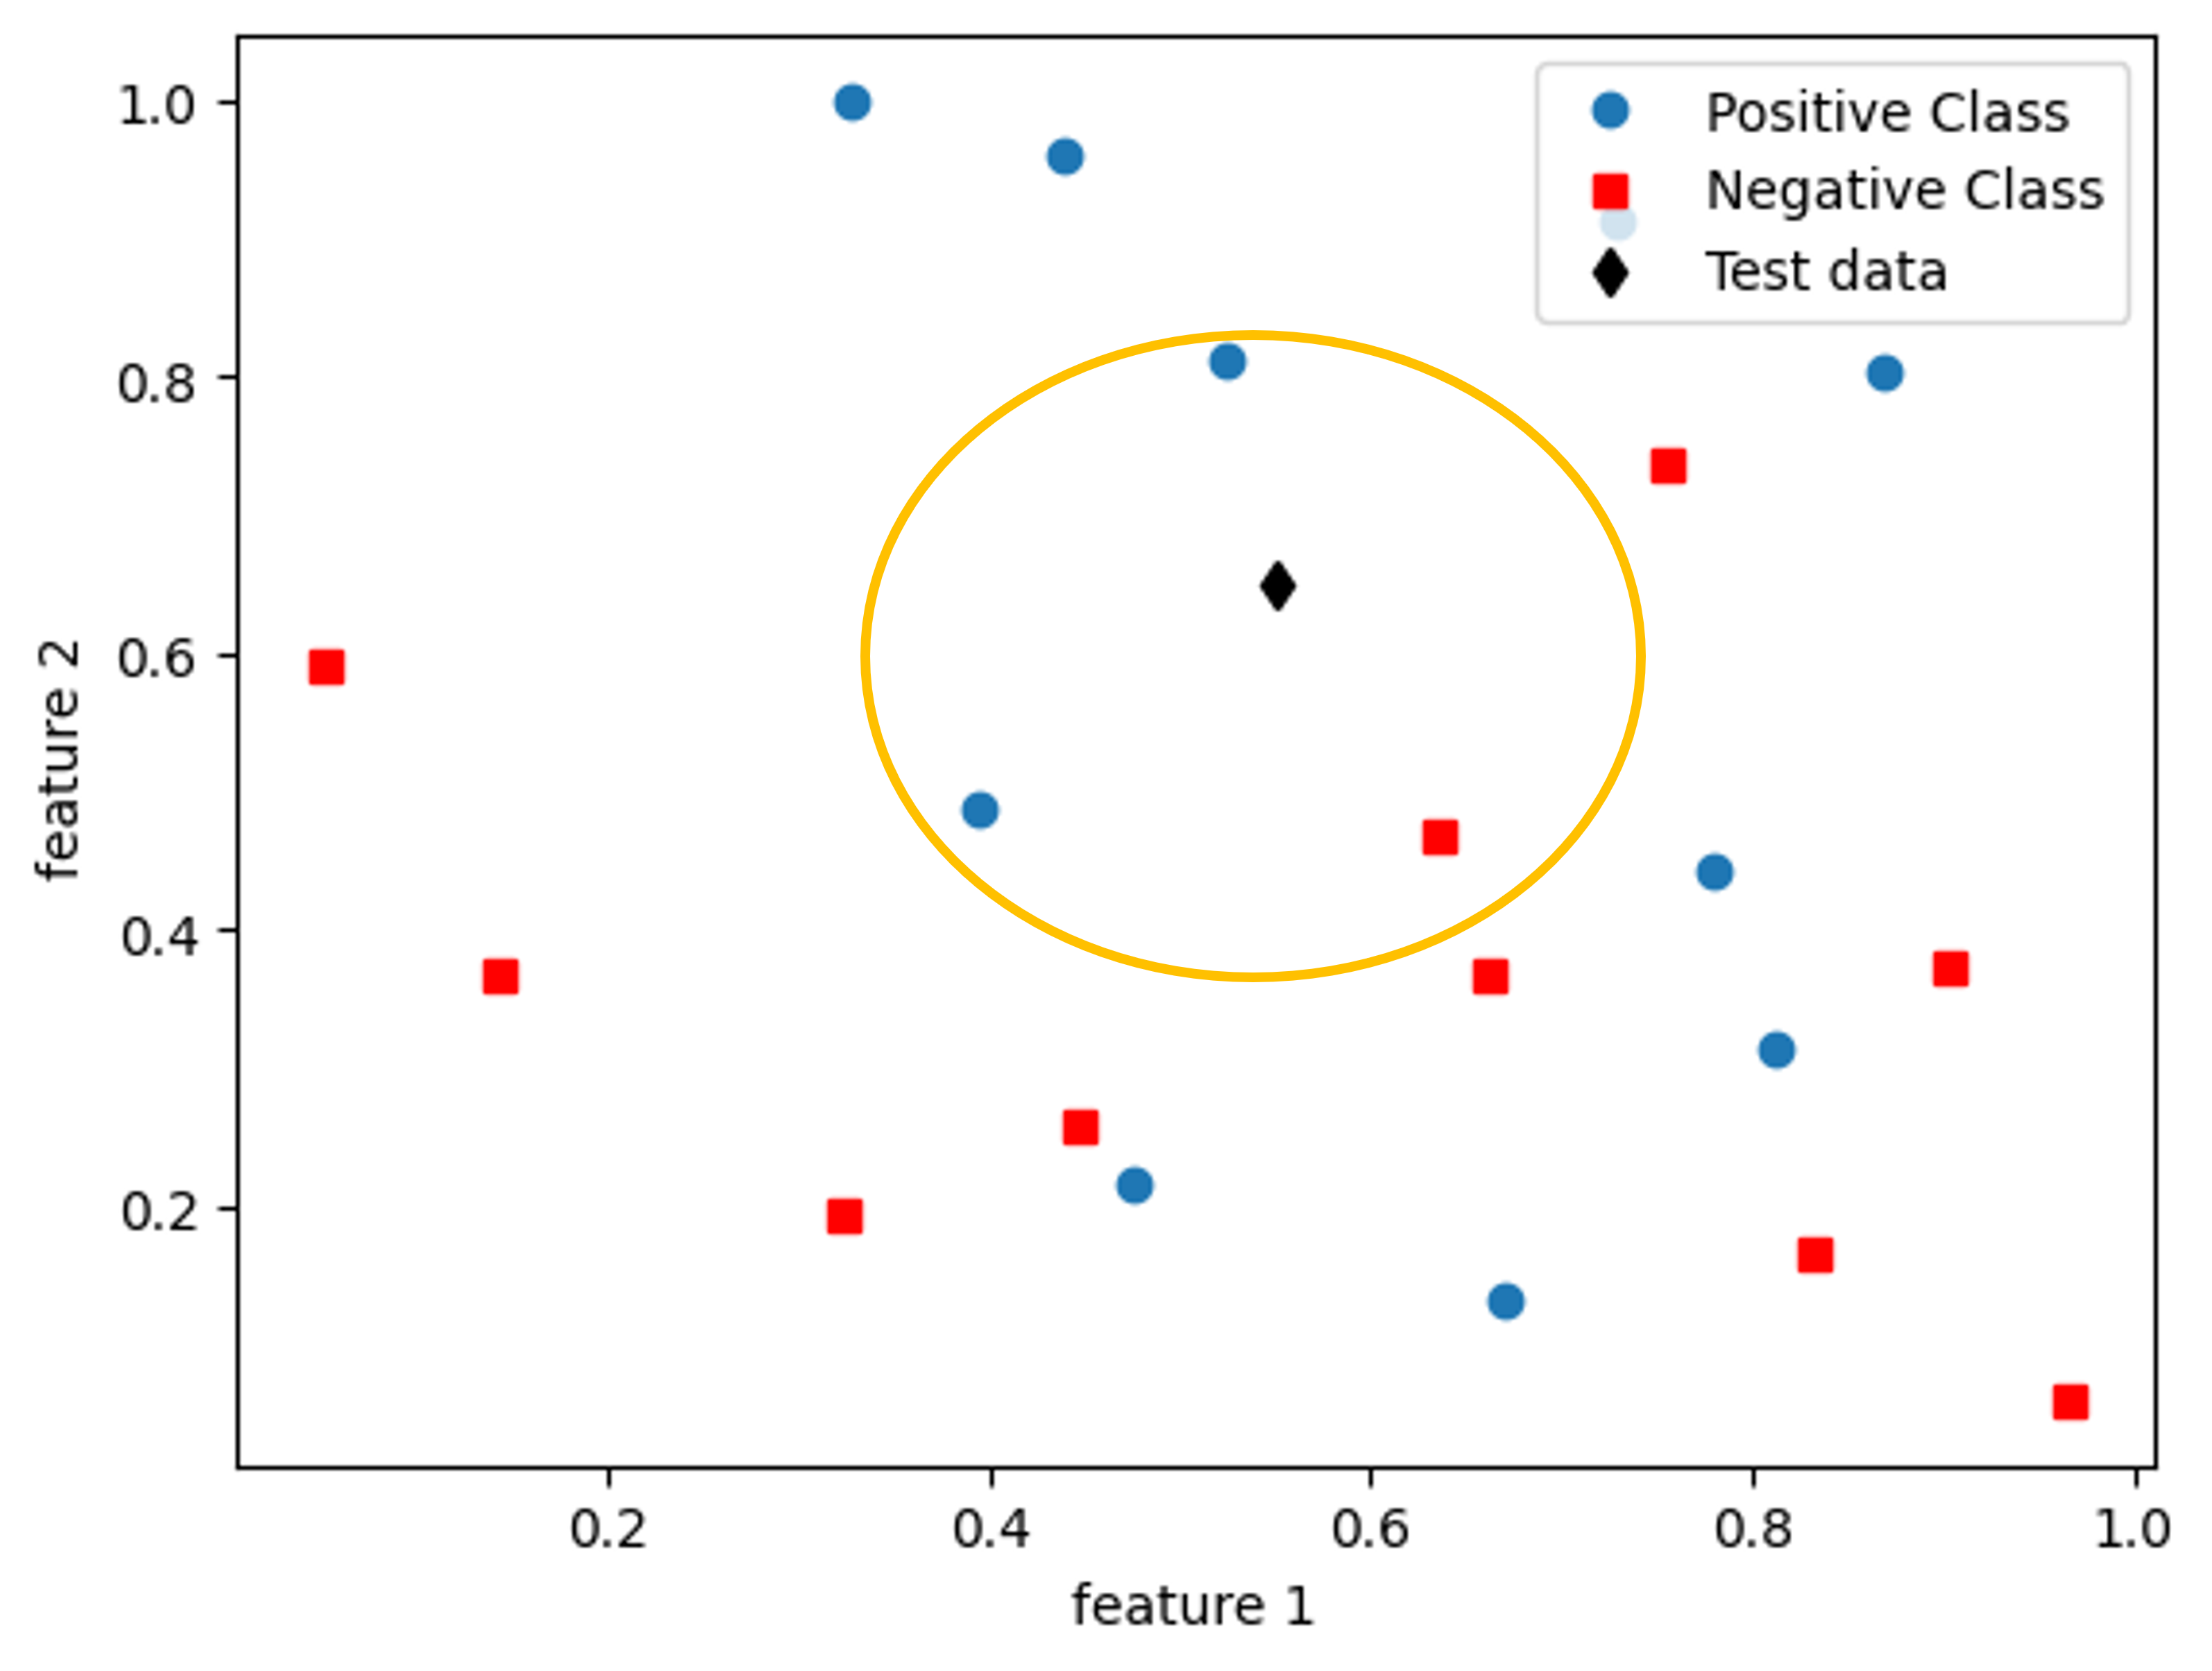
\includegraphics[width=7.5 cm]{knn_2.png}
  \caption{Concept of KNN}
  \label{fig:knn}
\end{figure}

The concept of k-NN is illustrated in Figure \ref{fig:knn}, using a simple example of a binary classification problem. The k-NN algorithm computes the distance between the new data point (represented by a black diamond) and all the data points in both the positive class (represented by blue circles) and the negative class (represented by red squares). In this example, the number of nearest neighbors is set to 3 (k = 3), as indicated by the yellow circle. In this case, two of the nearest neighbors of the test data belong to the positive class, and only one belongs to the negative class. As a result, the new data point will be assigned to the positive class.



\subsection{Distance Metrics in k-NN}
The initial step in k-NN is to calculate the distance from the new data point to all the other data points in the training data-set. One commonly used metric is the \textbf{Euclidean distance}, which measures the distance between two data points ($X_1$ and $X_2$) in an n-dimensional space. This distance is defined as:
\begin{equation}\label{eqn:eud}
  d(X_1, X_2) = \sum_{i=1}^n \sqrt{(x_1^i-x_2^i)^2}
\end{equation}

Another popular metric used in k-NN is the\textbf{ Manhattan distance}, which calculates the absolute distance between two data points and is defined as:

\begin{equation}\label{eqn:mah}
  d(X_1, X_2) = \sum_{i=1}^n \| x_1^i- x_2^i \|
\end{equation}

Other types of distance measures include Minkowski distance, cosine similarity, and Hamming distance.

\newpage
\subsection{Values of k in k-NN}
Another important parameter in the k-Nearest Neighbors (k-NN) method is the value of k, which represents the number of nearest neighbors that will be used to classify new data points. The choice of k can have a significant impact on the model's performance. A small value of k may result in a model that performs well on the training data set, but has high variance, meaning it may not generalize well to new, unseen data. On the other hand, a larger value of k may lead to a model with lower variance but higher bias, meaning it may not fit the training data as well.

\subsection{K-NN in Python}

The sample code below demonstrates how to implement the k-NN algorithm using Python.

\begin{lstlisting}
# ==================================================#
#--------------------------------------------------
## Using piepline to implement k-nn classifier ##
#--------------------------------------------------
from sklearn.neighbors import KNeighborsClassifier

steps = [('scaler', StandardScaler()),
         ('knn', KNeighborsClassifier(n_neighbors = 5))]
knn_pipeline = Pipeline(steps)
knn_pipeline.fit(X_train, y_train)
#--------------------------------------------------
## Model Evaluation ##
#--------------------------------------------------
from sklearn.metrics import classification_report
from sklearn.metrics import confusion_matrix
from sklearn.metrics import roc_auc_score


ypred_test = knn_pipeline.predict(X_test)
mat_clf = confusion_matrix(y_test, ypred_test)
report_clf = classification_report(y_test, ypred_test)

print(mat_clf)
print(report_clf)

ypred_testP = knn_pipeline.predict_proba(X_test)
auc = roc_auc_score(y_test, ypred_testP[:,1])
print(auc)
# ==================================================#
\end{lstlisting}

\newpage
\section{Support Vector Machine}
Support Vector Machine (SVMs) is a popular method for solving classification problems due to their strong performance. The goal of an SVM is to find a decision boundary that clearly separates different classes of data points.

In order to understand SVMs, it is important to be familiar with several key concepts, including: hyperplane, decision boundary, support vectors, margin, and SVM kernel.

\subsection{Hyperplane}
A hyperplane in geometry is a subspace of a vector space that has one dimension less than the vector space. For example, in a 2-dimensional vector space, a hyperplane is a line and in a 3-dimensional vector space, a hyperplane is a 2-dimensional plane (surface).

\subsection{Decision boundary}
A decision boundary is a line or \textbf{hyperplane} that divides different classes of data in a feature space, where a line is used in 2-dimensional space and a hyperplane is used in N-dimensional space, with N being the number of features.

Figure \ref{fig:svmEg} illustrates how decision boundaries can differ in 2-dimensional and 3-dimensional feature space. In 2D space, where there are only two features, classes can be separated by a straight line. However, in 3D space, the decision boundary becomes a plane. It can be difficult to envision in higher dimensional space, but most classification problems occur in higher dimensional space. Therefore, the SVM community typically refers to the decision boundary as a hyperplane in general. As demonstrated in Figure \ref{fig:svmEg}, more than one hyperplane can be used to separate the data into different classes.

\begin{figure}[!h]
  \centering
  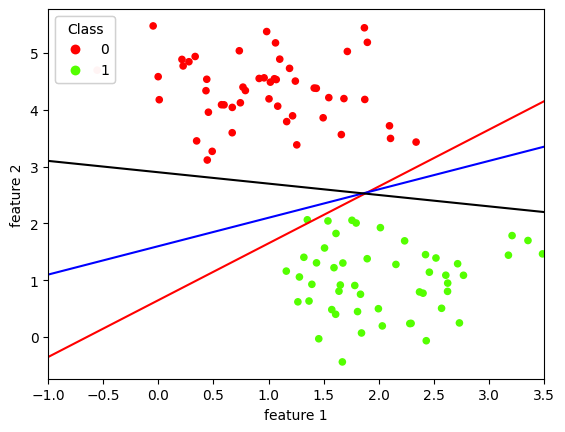
\includegraphics[width=4 cm]{svm_eg.png}
  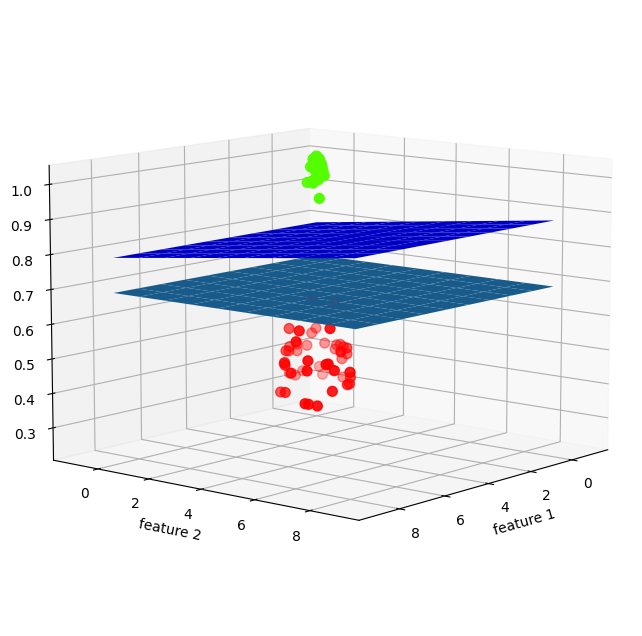
\includegraphics[width=4 cm]{svm_eg3d.png}
  \caption{Demonstration of SVM decision boundaries}
  \label{fig:svmEg}
\end{figure}

\subsection{Support Vectors}

SVM finds the hyperplane that separates the data points clearly by maximizing the gap between the decision boundary and the data points closest to it. These specific data points are known as "\textbf{support vectors}" in SVM.

\begin{figure}[!h]
  \centering
  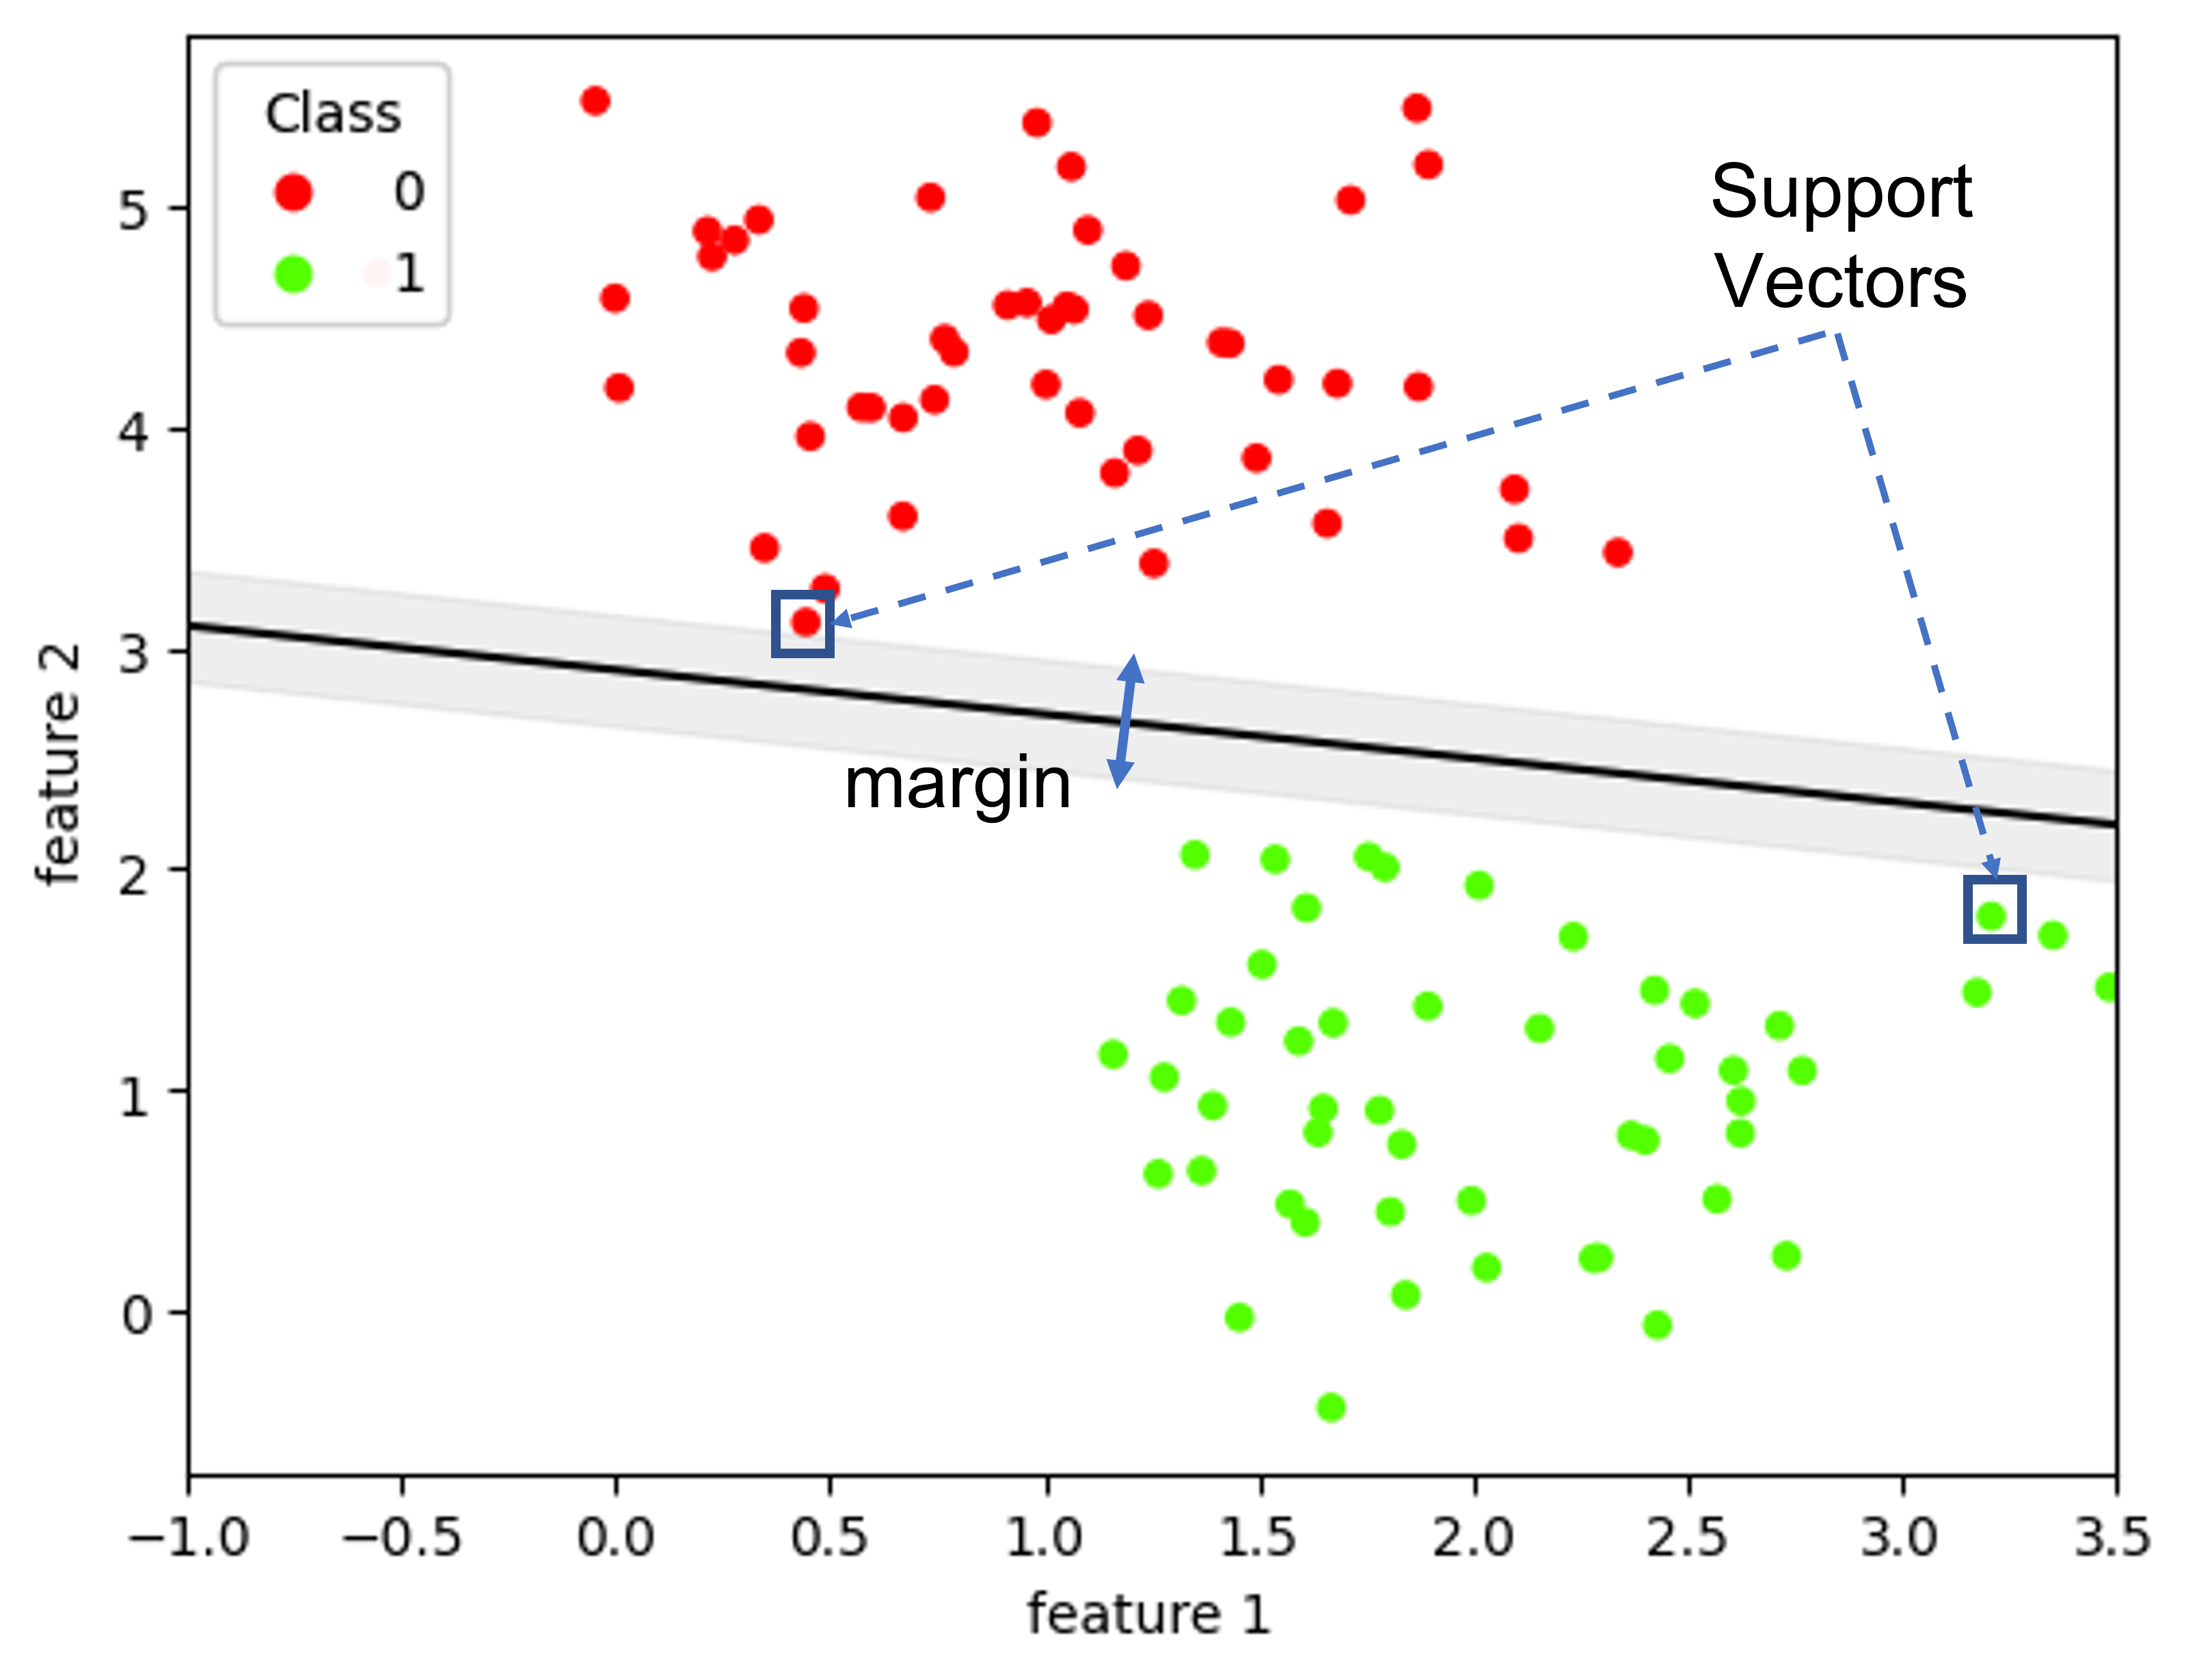
\includegraphics[width=8.0 cm]{svm_sv.png}
  \caption{Support Vectors in 2-Dimensional feature space}
  \label{fig:svm_SV}
\end{figure}

In Figure \ref{fig:svm_SV}, the support vectors are shown in the square box and removing these data points can alter the position and the orientation of the decision boundary.


%Hyperplane and decision boundary are equivalent at small dimension space, 'plane' has the meaning of straight and flat, so it is a line or a plane that separate the data sets. When you do a non-linear operation to map your data to a new feature space, the decision boundary is still a hyperplane in that space, but is not a plane any more at the original space.

%In the previous sections, we have learnt that logistic regression method finds a decision boundary (a line in 2-dimensional space) that minimizes the error between the predicted values and actual values. In other words, it maximizes the distance between the decision boundary and the data points. All the data points are considered in computing the distance.
%
%Similar to a linear regression/ logistic regression,  SVM maximizes the margin that has the maximum distance between the decision boundary and data points from both classes. SVM, instead of considering all data points like the linear regression, considers only the data points that are the closet to the decision boundary.

\subsection{Margin}
In SVM, the margin is the distance between the support vectors and the hyperplane, which is perpendicular. The goal of SVM is to find the maximum margin that can divide the data points between two classes. The margin is represented by the gray color in Figure \ref{fig:svm_SV}.

\subsection{SVM Kernels}
The data points shown in Figure \ref{fig:svm_SV} can be separated by a linear boundary, and SVM can identify the optimal hyperplane to distinguish between the two classes. However, in most real-world situations, the data points from different classes cannot be separated by a linear boundary. Figure \ref{fig:svm_K} shows an example of data points from two classes that cannot be separated by a linear boundary. One of the key advantages of SVM is its ability to use a kernel to classify non-linearly separable classes.

The role of a kernel is to change the data into a higher-dimensional space, making it possible for a hyperplane to distinguish different classes. There are various types of SVM-Kernels, and this section discusses three of them.

\begin{figure}[!h]
  \centering
  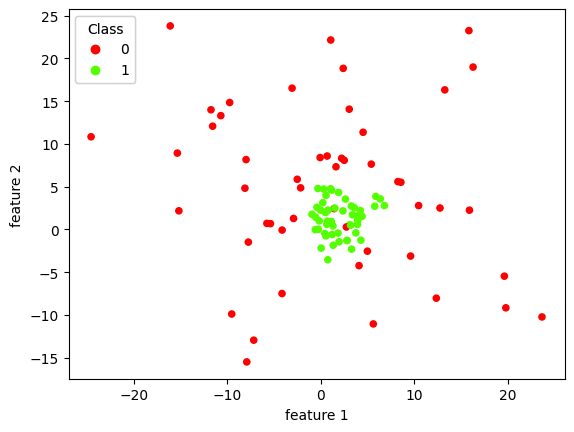
\includegraphics[width=8 cm]{svm_kernel.png}
  \caption{Linearly non-separable data set}
  \label{fig:svm_K}
\end{figure}

\newpage
\subsubsection{\textbf{Linear Kernel}}
A linear kernel is defined as:

\begin{equation}\label{eq:lin_kernel}
  K(X_1, X_2) = X_1^T X_2
\end{equation}This kernel is used only when the classes can be separated linearly.

\subsubsection{\textbf{Polynomial Kernel}}
A polynomial kernel utilizes a polynomial function to transform the data into a higher-dimensional space. The mathematical representation of this function is:

\begin{equation}\label{eq:poly_kernel}
  K(X_1, X_2) = (X_1^T X_2 + c)^d
\end{equation} where $c$ is the constant parameter and usually set at 0 or 1. $d$ is the degree (or order) of the polynomial function and $X_1$ and $X_2$ are n-dimensional data points.

Like polynomial regression, the degree $d$ is a hyper-parameter that controls the complexity of the kernel. The value of $d$ determines the degree of the polynomial function used to map the data into a higher-dimensional space. A higher degree of d means a more complex function, resulting in a more complex decision boundary, which can lead to over-fitting if the model is too complex for the data at hand.

On the other hand, a lower degree of $d$ means a simpler function and a simpler decision boundary, which can lead to under-fitting if the model is not complex enough to capture the underlying patterns in the data. Therefore, it is crucial to choose the appropriate degree d that balances the bias-variance trade-off as discussed in Section \ref{sec:hyperP}.


\subsubsection{\textbf{Radial Bias Function (RBF) kernel}}
RBF kernel computes the similarity between two data points $X_1$ and $X_2$ as follows:

\begin{equation}\label{eq:rbf}
  K(X_1, X_2) = \exp(-\gamma\|X_1-X_2\|^2)
\end{equation} where

\begin{equation}\label{eq:gamma}
  \gamma = \frac{1}{2\sigma^2}
\end{equation}and $\sigma$ is the variance of the kernel and control the width of the similarity region. $\|X_1-X_2\|$ is Euclidean ($L_2$-norm) distance between two data points $X_1$ and $X_2$.

\begin{figure}[!h]
  \centering
  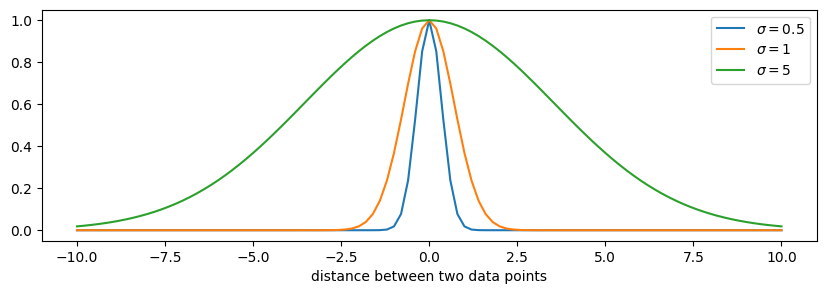
\includegraphics[width=8 cm]{kernel_dist.png}
  \caption{RBF kernel for different $\sigma$ values}
  \label{fig:kernel_d}
\end{figure}

The value of $\sigma$ decides which points should be considered as similar. Figure \ref{fig:kernel_d} illustrates how the $\sigma$ influences the region of the similarity. When the distance between two data points $\|X_1-X_2\|$ is zero, the value of the RBF kernel will always be one, regardless of the value of $\sigma$. Otherwise, the value of $\sigma$ affects the rate at which the RBF kernel decreases as the distance between two data points $\|X_1-X_2\|$  increases. When $\sigma$ is set to a low value, the RBF kernel decreases quickly, and when $\sigma$ is set to a high value, the RBF kernel decreases slowly. For example:

\begin{description}
  \item[case 1: $\sigma=0.5$] the value of the RBF kernel is zero when the distance is greater than 2.
  \item[case 2: $\sigma=1$] the value of the RBF kernel is zero when the distance is greater than 4.
  \item[case 3: $\sigma=5$] the value of the RBF kernel is zero only when the distance is greater than 10.
\end{description}


It is important to choose the appropriate value of $\sigma$ that balances the trade-off between over-fitting and under-fitting. A smaller value of $\sigma$ or a larger value of $\gamma$ may lead to over-fitting, as it only considers data points to be close if the distance between them is very small. The choice of the right value of the hyper-parameter $\gamma$ will significantly impact the performance of the RBF-SVM classifier.

\subsection{Hyper-parameters}

Hyper-parameter optimization plays a vital role in determining the performance of the SVM classifier. The key hyper-parameters that need to be considered are:

\subsubsection{\textbf{Kernel}}
The type of kernel is one of the hyper-parameters in implementing the SVM classifier, and the right choice of the kernel will lead to good performance. In Python, the grid or random search method can be used to find the right kernel.

\subsubsection{\textbf{Regularization parameter (C)}}
As discussed in Section \ref{sec:regularization}, a regularization term can be added to prevent the over-fitting and the parameter $C$ in Python sklearn controls the strength of the regularization. \href{https://www.csie.ntu.edu.tw/~cjlin/papers/guide/guide.pdf}{A practical guide to Support Vector Classifier} \cite{svmGuide:1984} guided that the value of the $C$ should be searched in the range of $C \in [2^{-5}, 2^15]$.

\subsubsection{\textbf{Degree (d)}}
In a polynomial kernel, the degree or order of the polynomial function is a hyper-parameter that needs to be tuned for the SVM classifier. Generally, the value of $d$ is set between 0 and 10.

\subsubsection{\textbf{Kernel coefficient ($\gamma$)}}
In RBF kernel, the value of $\gamma$ is an important hyper-parameter that needs to be selected. \href{https://www.csie.ntu.edu.tw/~cjlin/papers/guide/guide.pdf}{A practical guide to Support Vector Classifier} \cite{svmGuide:1984} guided the value of $\gamma$ should be searched within a range of $\gamma \in [2^{-15}, 2^3]$ to achieve optimal performance.

\newpage
\subsection{Linear SVM in Python}
The following code demonstrates how to implement a linear SVM classifier using the Python sklearn library.

\begin{lstlisting}
# ==================================================#
#--------------------------------------------------
## Using piepline to implement SVM classifier ##
#--------------------------------------------------
from sklearn.svm import SVC

steps = [('scaler', StandardScaler()),
         ('svc', SVC(kernel = 'linear'))]
svc_pipeline = Pipeline(steps)
svc_pipeline.fit(X_train, y_train)
#--------------------------------------------------
## Model Evaluation ##
#--------------------------------------------------
from sklearn.metrics import classification_report
from sklearn.metrics import confusion_matrix
from sklearn.metrics import roc_auc_score

ypred_test = svc_pipeline.predict(X_test)

mat_clf = confusion_matrix(y_test, ypred_test)
report_clf = classification_report(y_test, ypred_test)
auc = roc_auc_score(y_test, ypred_test)
# ==================================================#
\end{lstlisting}


\newpage
\subsection{Polynomial Kernel SVM in Python}

This section illustrates how to implement a non-linear SVM classifier using the polynomial kernel. The degree value $d$ is set at 5 in the SVC function. This hyper-parameter value can be adjusted using the ‘GridSearchCV’ method. The code for using the ‘GridSearchCV’ can be found in Section \ref{sec:hyperP}

\begin{lstlisting}
# ==================================================#
#--------------------------------------------------
## Using piepline to implement SVM Poly classifier ##
#--------------------------------------------------
from sklearn.svm import SVC

steps = [('scaler', StandardScaler()),
         ('svc', SVC(kernel = 'poly', degree = 5))]

svc_pipeline = Pipeline(steps)
svc_pipeline.fit(X_train, y_train)

#--------------------------------------------------
## Model Evaluation ##
#--------------------------------------------------
from sklearn.metrics import classification_report
from sklearn.metrics import confusion_matrix
from sklearn.metrics import roc_auc_score

ypred_test = svc_pipeline.predict(X_test)

mat_clf = confusion_matrix(y_test, ypred_test)
report_clf = classification_report(y_test, ypred_test)
auc = roc_auc_score(y_test, ypred_test)
# ==================================================#
\end{lstlisting}

\newpage
\subsection{RBF Kernel SVM in Python}
The following code demonstrates how to implement the RBF kernel using Python. The gamma value is set to $\gamma = \frac{1}{N\sigma_X}$ which is defined as a default value in the Python sklearn library and referred to as `scale'.
\begin{lstlisting}
# ==================================================#
#--------------------------------------------------
## Using piepline to implement SVM RBF classifier ##
#--------------------------------------------------
from sklearn.svm import SVC

steps = [('scaler', StandardScaler()),
         ('svc', SVC(kernel = 'rbf', gamma = 'scale'))]

svc_pipeline = Pipeline(steps)
svc_pipeline.fit(X_train, y_train)

#--------------------------------------------------
## Model Evaluation ##
#--------------------------------------------------
from sklearn.metrics import classification_report
from sklearn.metrics import confusion_matrix
from sklearn.metrics import roc_auc_score

ypred_test = svc_pipeline.predict(X_test)

mat_clf = confusion_matrix(y_test, ypred_test)
report_clf = classification_report(y_test, ypred_test)
auc = roc_auc_score(y_test, ypred_test)
# ==================================================#
\end{lstlisting}

%\section{Naïve Bayes’ Classifier}
%A Naïve Bayes’ Classifier is a probabilistic machine learning method that is based on the Bayes’ theorem.
%
%In Bayes’ theory, the probability for the output $y$ (a class label) is given by.
%Byaes theorem states that p(y j x) describes the
%probability for the output y (a class label) given that we know the input x.
%\subsection{Bernoulli Naive Bayes}
%\subsection{Multinomial Naive Bayes}
%\subsection{Gaussian Naive Bayes}
%\subsection{Implementation in Python}

\newpage
\section{Naive Bayes Classifier}
\epigraph{If you do well in the mid-term exam, will you do well in the final exam?}

Factors such as continued study and preparation, the difficulty of the final exam, and the student's personal abilities and circumstances play a role in determining their performance on the final exam. However, in general, a good score in the mid-term exam can indicate a higher likelihood of success on the final exam. The probability of an event (passing final exam) depends on prior knowledge or information about the mid-term exam.

\subsection{Bayes' Theorem}
Thomas Bayes, an 18th-century statistician and mathematician, developed Bayes' Theorem, which is a mathematical formula that describes the relationship the relationship between the probability of an event and the prior information.

\begin{equation}\label{eqn:Bayes}
  P(A\|B) = \frac{P(B)P(B\|A)}{P(A)}
\end{equation} where $P(A\|B)$ is the probability of A happening, given that B has occurred and $P(B\|A)$ is the reverse conditional probability of event B given that event A has occurred. $P(B)$ is the prior probability of event B and $P(A)$ is the prior probability of event A.

Imagine that there are 20 students in the class. 16 out of 20 students passed the mid-term exam but only 15 students passed the final exam. Among the students who passed the final exam, 14 students passed the mid-term exam. Using the Bayes' Theorem, the probability of passing the final exam given that the student passed the mid-term exam can be calculated as below:

\begin{itemize}
  \item The probability of passing the final exam, without considering the relationship with the mid-term exam, is $P(A) = 15/20 = 0.75 \text{\hspace{5pt}or \hspace{5pt}} 75\%$.
  \item The probability of passing the mid-term exam, given that the student passed the final exam, is $P(B | A) = 14/15 = 0.93 \text{\hspace{5pt}or \hspace{5pt}}  93\%$.
  \item The probability of passing the mid-term exam is $P(B) = 16/20 = 0.8 \text{\hspace{5pt}or \hspace{5pt}} 80\%$.
\end{itemize}

Therefore, the probability of passing the final exam, given that the student passed the mid-term exam, is
\begin{eqnarray}
% \nonumber to remove numbering (before each equation)
  P(A | B) &=& \frac{P(B | A) * P(A)} {P(B)} \\
           &=& \frac{0.93 * 0.75}{0.80}\\
           &=& 0.87  \text{\hspace{5pt}or \hspace{5pt}} 87\%
\end{eqnarray}

Bayes' Theorem shows that if the student pass the mid-term exam, he or she has a higher chance (87\%) of passing the final exam. This theorem is helpful to predict the posterior probability of an event with some prior knowledge.

\newpage
\subsection{Naive Bayes classifier}
A Naive Bayes classifier is a \textbf{probabilistic} machine learning method based on Bayes' Theorem. This method assumes that the features are independent and have an equal effect on the outcome. Going back to the previous example, we want to classify the student is going to pass the final exam or not based on the score of the mid-term exam and attendance scores of a student. Naive Bayes classifier assumes that the performance in the mid-term exam does not depend on the attendance scores and both features have the equal effect on the final exam.

According to the Baye's Theorem, the probability of passing the final exam is
\begin{equation}\label{eqn:NBclassifier}
% \nonumber to remove numbering (before each equation)
  P(y | x_1, x_2) = \frac{P(x_1 | y) * P(x_2|y) * P(y)} {P(x_1)*P(x_2)} \\
\end{equation}


The variable y is the class variable (pass or fail). Variable $x_1$ and $x_2$ represent the parameters/features. This is an example of binary classification where the class `y' has only two outputs (pass or fail). The Naive Bayes classifier then calculates the probabilities for both passing and failing the final exam and assigns the class with the highest probability as the prediction.
\begin{equation}\label{eqn:NBbinary}
% \nonumber to remove numbering (before each equation)
  y = \left\{
        \begin{array}{ll}
          pass, & \hbox{$P(y= \text{pass} | x_1, x_2)> P(y= \text{fail} | x_1, x_2)$;} \\
          fail, & \hbox{otherwise.}
        \end{array}
      \right.
\end{equation}

For multi-class classification, the equation \ref{eqn:NBbinary} can be defined as:
\begin{equation}\label{eqn:NBbinary}
% \nonumber to remove numbering (before each equation)
  y = \arg\max_y \left(P(y) \prod_{i=1}^n P(x_i|y)\right)
\end{equation}

This method is called "naive" because it assumes that the features are independent, which may not always be the case in real-world situations. However, despite its limitations, Naive Bayes classifiers are fast, simple and often perform well in practice.

\newpage
\subsection{Types of Naive Bayes Classifier}

There are three main types of Naive Bayes classifiers:

\subsubsection{\textbf{Multinomial Naive Bayes}}
It is mainly used for text classification problems and assumes that features are discrete and count-based.

\subsubsection{\textbf{Bernoulli Naive Bayes}}
It is similar to the Multinomial Naive Bayes but assumes binary occurrence of features. The features are boolean variable and can either be present (yes) or absent (no).

\subsubsection{\textbf{Gaussian Naive Bayes}}
It assumes that the features are normally distributed and calculates the probabilities of each class based on the mean and variance of the features. The conditional probability of the independent variable $x_i$ given that the event y occurs is:
\begin{equation}\label{eqn:NBGauss}
% \nonumber to remove numbering (before each equation)
  P(x_i|y) = \frac{1}{\sqrt{2\pi\sigma^2}}\exp\left(-\frac{(x_i - \mu)^2}{2\sigma^2}\right)
\end{equation} where $\mu$ and $\sigma$ are mean and variance of the feature $x_i$ for the class $y$.


\newpage

\subsection{Implementation in Python}
The following code demonstrates how to implement the  Naive Bayes Classifier using Python sklearn library.

\begin{lstlisting}
# ==================================================#
#--------------------------------------------------
## Gaussian NB classifier ##
#--------------------------------------------------
from sklearn.naive_bayes import GaussianNB

gnb = GaussianNB()
gnb.fit(X_train, y_train)
#--------------------------------------------------
## Multinomial NB Classifier ##
#--------------------------------------------------
from sklearn.naive_bayes import MultinomialNB

mnb = MultinomialNB(alpha=1.0)
mnb.fit(X_train, y_train)
#--------------------------------------------------
## Bernoulli NB Classifier ##
#--------------------------------------------------
from sklearn.naive_bayes import BernoulliNB
bnb = BernoulliNB(alpha=1.0)
bnb.fit(X_train, y_train)
# ==================================================#
\end{lstlisting}
\newpage
\section{Project: Fraud Detection}\label{sec:cls_proj1}
There are many other types of classifiers such as tree-based classifiers, random forest, and deep learning methods that are not covered in this book. Deep learning methods have been extensively used in many research publications.

However, many researchers and practitioners have pointed out that the choice of a machine learning method depends on various factors, including the specific problem, the size and complexity of the data-set, and the computational resources available.

In this section, we will present the full codes for fraud detection using Logistic Regression, K-NN, and SVM classifiers. We will also compare the performance of these classifiers using the 'accuracy' and 'recall' metrics discussed in Section \ref{sec:Clsevaluation}.

The data-set \cite{web:fraudData} used in this analysis contains $21,693$ entries and $29$ independent features. This data-set is imbalanced, with $21,337$ non-fraud cases and $356$ fraud cases. The data is already cleaned and there is no missing data. The data-set can be downloaded from \href{https://github.com/yonycherkos/Applied-Data-Science-with-Python-Specialization.git}{the link provided} \cite{web:fraudData}.

\newpage
\subsection{Data Importing}
The first step is to import the necessary modules and import the data from the computer.

\begin{lstlisting}
# ==================================================#
import pandas as pd

df=pd.read_csv('..\\data\\fraud.csv', index_col = 0)
y = df['Class'].values
df = df.iloc[:,1:]
X = df.drop(columns = 'Class').values
# ==================================================#
\end{lstlisting}

\subsection{Splitting the data}

The next step is to divide the data into a training dataset and a testing dataset. 60\% of the data is allocated for training and the remaining 40\% is reserved for testing.

\begin{lstlisting}
# ==================================================#
from sklearn.model_selection import train_test_split

X_train, X_test, y_train, y_test = train_test_split(X,y,
                                    test_size = 0.40,
                                    random_state=1)
# ==================================================#
\end{lstlisting}

\subsection{Modelling}
Five different classifiers are developed. The names and hyper-parameters of the classifiers are provided in Table \ref{tb:clf_parameters}.
Regularization is added to all classifiers, except K-NN and the strength of regularization is controlled by the parameter $C$. In logistic regression, the $L2$ term is used for regularization and squared $L2$ is used for SVM classifiers.

The number of neighbors in K-NN is controlled by the value of $k$ and the order or degree of the polynomial function in SVM is defined as $3$. The kernel coefficient $\gamma$ for SVM-RBF kernel is defined as $\gamma = \frac{1}{N\sigma_{Xtr}}$.

\begin{table}[!ht]
\centering
\begin{tabular}{|c|c|c| }
  \hline
  Name & \multicolumn{2}{|c|}{Hyper-parameters}\\
  \hline
  LR  & C = 1.0& \\
  \hline
  KNN & k = 5  & \\
  \hline
  SVM-Linear & C = 1.0 &   \\
  \hline
  SVM-Poly &  C = 1.0  &  degree = 3\\
  \hline
  SVM-RBF & C = 1.0    & $\gamma = \frac{1}{N\sigma_{Xtr}}$\\
  \hline
\end{tabular}
\caption{Classifier model and its hyper-parameters}\label{tb:clf_parameters}
\end{table}

\newpage
\begin{lstlisting}
# ==================================================#
from sklearn.preprocessing import StandardScaler
from sklearn.pipeline import Pipeline
#--------------------------------------------------
## ------------Logistic Regression----------------##
#--------------------------------------------------

from sklearn.linear_model import LogisticRegression

steps = [('scaler', StandardScaler()),
         ('logReg', LogisticRegression(penalty = "l2",
                                        C = 1.0))]

LR_pipeline = Pipeline(steps)
LR_pipeline.fit(X_train, y_train)
#--------------------------------------------------
## ----------- K-NN Classifier ------------------##
#--------------------------------------------------

from sklearn.neighbors import KNeighborsClassifier

steps = [('scaler', StandardScaler()),
         ('knn', KNeighborsClassifier(n_neighbors = 5))]

knn_pipeline = Pipeline(steps)
knn_pipeline.fit(X_train, y_train)
#--------------------------------------------------
## ------------ SVM Classifier ------------------##
#--------------------------------------------------
from sklearn.svm import SVC
## Linear Kernel  ---------------
steps = [('scaler', StandardScaler()),
         ('svc', SVC(kernel = 'linear',
                     class_weight='balanced'))]

svcL_pipeline = Pipeline(steps)
svcL_pipeline.fit(X_train, y_train)
## Polynomial Kernel -----------------------
steps = [('scaler', StandardScaler()),
         ('svc', SVC(kernel = 'poly', degree = 3,
                     class_weight='balanced'))]

svcPoly_pipeline = Pipeline(steps)
svcPoly_pipeline.fit(X_train, y_train)
## RBF Kernel -----------------------
steps = [('scaler', StandardScaler()),
         ('svc', SVC(kernel = 'rbf', gamma = 'scale',
                     class_weight='balanced'))]

svcRBF_pipeline = Pipeline(steps)
svcRBF_pipeline.fit(X_train, y_train)
# ==================================================#
\end{lstlisting}

\subsection{Model Evaluation}
The classifiers are evaluated using three metrics: 'accuracy', 'recall', and 'area under the curve'. As discussed in Section \ref{sec:Clsevaluation}, 'recall' is an essential metric for fraud detection as we do not want to miss any fraud case. It is better to have false alarms than missing a fraud. The following codes calculate the metrics using the \emph{classification report function} under sklearn.metrics module  and extract the accuracy and recall parameters. The function roc\-auc\_score is used to compute the area under the curve. The evaluation is done for both the training and testing sets, and the results are saved in a tabular format.

\begin{lstlisting}
# ==================================================#
from sklearn.metrics import classification_report
from sklearn.metrics import roc_auc_score

result_df = pd.DataFrame(columns = ['Tr_accuracy',
                                    'Test_accuracy',
                                    'Tr_recall',
                                    'Test_recall',
                                    'Train_auc',
                                    'Test_auc'])

model_name = [LR_pipeline, knn_pipeline, svcL_pipeline,
              svcPoly_pipeline, svcRBF_pipeline]
for idx, model in enumerate(model_name):
    ## for training data
    ypred_train = model.predict(X_train)
    report_clf = classification_report(y_train,
                                       ypred_train,
                                       output_dict=True)
    df_r = pd.DataFrame(report_clf).transpose()
    acc_tr = df_r.loc['accuracy', 'recall'].round(3)
    recall_tr = df_r.iloc[1,1].round(3)
    auc_tr = roc_auc_score(y_train, ypred_train)
    ## for testing data
    ypred_test = model.predict(X_test)
    report_clf = classification_report(y_test,
                                       ypred_test,
                                       output_dict=True)
    df_r = pd.DataFrame(report_clf).transpose()
    acc = df_r.loc['accuracy', 'recall'].round(3)
    recall = df_r.iloc[1,1].round(3)
    auc = roc_auc_score(y_test, ypred_test)

    result_df.loc[idx,:]=[acc_tr, acc, recall_tr,
                          recall, auc_tr.round(3),
                          auc.round(3)]
result_df.index = ['LR', 'K-NN', 'SVM-Linear',
                   'SVM-Poly', 'SVM-RBF']
# ==================================================#
\end{lstlisting}

\subsection{Discussion on Performance}

\subsubsection{\textbf{Accuracy}}

Table \ref{tb:accR} lists the accuracy scores for different classifiers. The SVM-linear model performs the worst with an accuracy score of 97\%. The performance is similar for both the training and testing sets.

However, as discussed in Section \ref{tb:clf_parameters}, accuracy score is not a good measure for imbalanced classes. Our data-set has 98\% of non-fraud cases and only 2\% of fraud cases. This is a common scenario in many problems such as cancer detection, spam detection, etc. The negative class (class 0) always has more data than the positive class (class 1).

\begin{table}[!ht]
\centering
\csvreader[tabular=|c|r|r|, ,table head=\hline & Train & Test \\\hline, late after line=\\\hline]%
{data/accuracy.csv}{Name= \Name, Train=\Train, Test=\Test}{\Name & \Train & \Test}
\caption{Accuracy for Fraud Detection using different methods.}\label{tb:accR}
\end{table}

\subsubsection{\textbf{Recall}}

Table \ref{tb:accR} lists the recall values for different classifiers. The SVM with the RBF kernel performs the best with a score of 99\% for the training data-set. It means that 99\% of the fraud cases in the training set are successfully detected by the SVM-RBF classifier. However, it can be observed that the SVM-RBF over-fits the training data, and it performs the worst for the testing data-set. The SVM classifier with the linear model produces reasonable results for both the training and testing data-sets at 91\% and 88\% respectively. The SVM-linear classifier has a good balance between bias and variance.

\begin{table}[!ht]
\centering
\csvreader[tabular=|c|r|r|, ,table head=\hline & Train & Test \\\hline, late after line=\\\hline]%
{data/recall.csv}{Name= \Name, Train=\Train, Test=\Test}{\Name & \Train & \Test}
\caption{Recall for Fraud Detection using different methods.}\label{tb:recallR}
\end{table}

\subsubsection{\textbf{Area under the Curve}}
Table \ref{tb:accR} lists the areas under the curve for fraud detection using different classifiers. Similar to the recall score, the SVM classifier with the linear model produces the best results (94\% for training and 92.7\% for testing set) without over-fitting the problem.

\begin{table}[!ht]
\centering
\csvreader[tabular=|c|r|r|, ,table head=\hline & Train & Test \\\hline, late after line=\\\hline]%
{data/auc.csv}{Name= \Name, Train=\Train, Test=\Test}{\Name & \Train & \Test}
\caption{Area under the curve using different methods.}\label{tb:aucR}
\end{table}

The results from this project suggest that the complexity of the model does not always lead to better performance. Higher model complexity can cause over-fitting, leading to high variance in the results. Hyper-parameters can be adjusted to enhance the performance of the classifier.

%\section{Project: Sentiment Analysis}\label{sec:cls_proj2}
%This section presents how to perform text classification using a logistic regression, SVM and Naïve Bayes’ classifiers. The objective of the project is to classify if a technology is in demand or not using the data-set provided by the O*NET-Resource center. (talk about the data) United Nations Standard Products and Services Code (UNSPSC).
%
%In this project, the independent variable is `text' that describes the Commodity Title of a technology defined by O$*$NET and the target is either `yes (In demand)' or `no (not in demand)'. Compared to the previous project, the input feature is a text with different lengths and this feature can not be directly used in machine learning algorithms. Some examples of input variables are listed in Table.
%
%\subsection{Text Vectorization}
%Text Vectorization is the process of transforming raw data (text) into numerical features that can be processed while preserving the information in the original data set.
%
%\subsubsection{\textbf{TF-IDF}}
%TF-IDF stands for “Term Frequency — Inverse Document Frequency” and it is one of the most commonly used features in text analysis. TF-IDF transforms the text with different lengths to a common vector space.
%\begin{equation}\label{TF}
%  TF-IDF = TF*IDF
%\end{equation}
%
%
%\subsubsection{\textbf{Term Frequency}}
%The word `Term' refers to the 'word' in a sentence or a document and `Frequency' refers to the number of times that a particular item occurs. Hence `Term Frequency' refers to the \emph{number of times the term appears in a document compared to the total number of words in the document}.
%
%\begin{equation}\label{TF}
%  TF = \frac{\text{number of times the term appears in a document}}{\text{total number of words in the document}}
%\end{equation}
%
%
%\subsubsection{\textbf{Inverse Document Frequency}}
%Inverse Document Frequency of a term reflects the proportion of documents in the corpus (a large collection of documents) that contain the term.
%
%\begin{equation}\label{IDF}
%  TF = \log\left(\frac{\text{number of documents in the corpus}}{\text{number of documents that contain the term}}\right)
%\end{equation}
%
%
%\subsubsection{Word2Vec}
%\subsubsection{BERT}
%
%\subsection{Modeling} 

\chapter{Further Reading}

This book provides an overview of the basic concepts in machine learning, including linear and polynomial regression and parametric classifiers such as logistic regression and SVM, as well as non-parametric classifiers like K-NN. However, it should be noted that there are many other machine learning techniques such as gradient boosting, tree-based classifiers, random forest, and deep learning methods that are not covered in this book.

Deep learning methods have become increasingly popular in recent years and are often highlighted in research publications. However, it's important to keep in mind that the choice of a machine learning method should be based on factors such as the specific problem, the size and complexity of the data-set, and the available computational resources. Many researchers and practitioners in industry stress the importance of considering these factors when choosing a machine learning method.

ChatGPT \cite{web:chatgpt} recommends the following math topics, online courses, and books for beginners interested in studying machine learning. This chapter is included to show how AI tools can be used to enhance the effectiveness and efficiency of educators and learners. It's important to note that the field of machine learning is constantly evolving, and this list may not always be up to date. Therefore, it's important not to rely solely on the recommendations provided by ChatGPT and to choose resources that align with your learning style. However, the list provided by ChatGPT can serve as a useful starting point for quickly and comprehensively learning about the field

\textbf{The list is not comprehensive and generated by ChatGPT \cite{web:chatgpt}. }


\newpage
\section{Mathematic Topics recommended by ChatGPT}
Mathematics plays a crucial role in understanding machine learning methods, and ChatGPT has suggested the following topics as important to learn.

\begin{itemize}
  \item Linear Algebra:  understanding concepts such as matrix operations, eigenvalues and eigenvectors, and singular value decomposition. Linear algebra is used in many machine learning algorithms, including neural networks, principal component analysis (PCA), and singular value decomposition (SVD).
  \item Calculus: understanding concepts such as derivatives and gradients, which are used in optimization algorithms such as gradient descent.
  \item Probability and Statistics: understanding concepts such as probability distributions, Bayes' theorem, and hypothesis testing. These concepts are used in many machine learning algorithms, including Bayesian networks and Gaussian mixture models.
  \item Optimization: understanding concepts such as convex optimization, gradient descent, Newton's method etc. which are used in many machine learning algorithms, including linear regression and support vector machines.
  \item Information theory and entropy: understanding of the concept of entropy, mutual information, and cross-entropy which are used in many machine learning algorithms such as decision tree, information gain, and KL divergence.
\end{itemize}

\newpage
\section{Courses recommended by ChatGPT}
There are many different platforms that offer machine learning-related courses, including LinkedIn, Coursera, Edx, Udemy, Udacity, and DataCamp. The list provided below is based on ChatGPT's suggestions. It's recommended to select one of these courses to begin your learning journey and assess if it aligns with your preferred method of learning.

\begin{itemize}
  \item "Introduction to Machine Learning" by Andrew Ng on Coursera
  \item "Machine Learning" by Georgia Tech on Udacity
  \item "Deep Learning" by Andrew Ng on Coursera
  \item "Applied Data Science with Python" on Coursera
  \item "Introduction to Machine Learning with Python" by Sarah Guido and Andreas Müller on Coursera
  \item "Machine Learning A-Z: Hands-On Python and R In Data Science" by Kirill Eremenko and Hadelin de Ponteves on Udemy
  \item "Machine Learning for Data Science and Analytics" by Columbia University on edX
\end{itemize}


\newpage
\section{Books recommended by ChatGPT}
Online courses can be a fast and convenient way to learn a topic, but it's important to be aware that not all courses are of equal quality. Some courses may be high-quality and effective in helping you to quickly grasp a topic, while others may be low-quality and not worth your time and energy. In some cases, low-quality courses can even discourage you from continuing your learning journey. While online courses can be a great resource, traditional methods like books can also provide a solid foundation for learning.

The following books are recommended by ChatGPT. I am particularly pleased to see "Pattern Recognition and Machine Learning" as the first recommendation, as it was the textbook I used during my undergraduate studies in 2003.

\begin{itemize}
   \item "Pattern Recognition and Machine Learning" by Christopher M. Bishop: This book provides a comprehensive introduction to the field of machine learning and covers a wide range of topics, from the basics of probability and statistics to advanced machine learning techniques.

   \item "Deep Learning" by Yoshua Bengio, Ian Goodfellow, and Aaron Courville: This book provides a comprehensive introduction to deep learning, including the theory and practice of training deep neural networks.

   \item "Machine Learning: A Probabilistic Perspective" by Kevin P. Murphy: This book provides a comprehensive introduction to machine learning from a probabilistic perspective and covers a wide range of topics, from supervised learning to unsupervised learning and Bayesian methods.

   \item "Introduction to Machine Learning" by Alex Smola and S.V.N. Vishwanathan : This book provides an introduction to machine learning and covers a wide range of topics, including supervised learning, unsupervised learning, and reinforcement learning.

   \item "The Hundred-Page Machine Learning Book" by Andriy Burkov: This book is a concise and accessible introduction to machine learning, providing an overview of the most important concepts and algorithms in the field.

   \item "Python Machine Learning" by Sebastian Raschka and Vahid Mirjalili: This book provides a hands-on introduction to machine learning using Python, including coverage of a wide range of machine learning algorithms and libraries.

   \item "Machine Learning for Dummies" by John Paul Mueller: This book provides an easy-to-understand introduction to the basics of machine learning, including supervised and unsupervised learning techniques.

   \item "Hands-On Machine Learning with Scikit-Learn, Keras, and TensorFlow" by Aurélien Géron: This book provides an in-depth introduction to machine learning using popular Python libraries such as Scikit-Learn, Keras, and TensorFlow.
\end{itemize}







\bibliographystyle{unsrt} % We choose the "plain" reference style
\bibliography{refs}


\end{document} 